\documentclass[11pt, letterpaper, openany]{book}
\usepackage[utf8]{inputenc}
\usepackage[T1]{fontenc}
\usepackage{lmodern}
\usepackage{microtype}
\usepackage{geometry}
\geometry{margin=1in}
\usepackage{float}
\usepackage{amsmath, amssymb, amsfonts}
\usepackage{graphicx}
\usepackage{xcolor}
\usepackage{tikz}
\usepackage{colortbl}
\usetikzlibrary{shapes, arrows.meta, positioning, patterns, decorations.pathreplacing, calc}
\usepackage{listings}
\usepackage{xurl}
\usepackage{hyperref}
\usepackage{fancyhdr}
\usepackage{titlesec}
\usepackage{setspace}
\usepackage{tcolorbox}
\usepackage{booktabs}
\usepackage{array}
\usepackage{longtable}
\usepackage{multirow}

% --- Kish Lattice Color Definitions ---
\definecolor{kishblue}{RGB}{0, 50, 120}
\definecolor{goldseal}{RGB}{184, 134, 11}
\definecolor{codegreen}{rgb}{0,0.6,0}
\definecolor{codegray}{rgb}{0.5,0.5,0.5}
\definecolor{signalgreen}{RGB}{0,140,0}
\definecolor{signalred}{RGB}{180,0,0}
\definecolor{floorblue}{RGB}{0, 100, 200}
\definecolor{newgold}{RGB}{180, 140, 0}
\definecolor{cruciblered}{RGB}{170, 45, 10}
\definecolor{formgray}{RGB}{90, 90, 90}
\definecolor{spectroviolet}{RGB}{90, 0, 150}
\definecolor{dimensionred}{RGB}{160, 20, 20}
\definecolor{aperblue}{RGB}{20, 90, 140}
\definecolor{luminorange}{RGB}{255, 140, 0}
\definecolor{theorytag}{RGB}{200, 50, 50}
\definecolor{vectorteal}{RGB}{0, 120, 120}


\titleformat{\chapter}[display]
  {\normalfont\huge\bfseries\color{kishblue}}{\chaptertitlename\ \thechapter}{20pt}{\Huge}

\pagestyle{fancy}
\fancyhf{}
\fancyhead[L]{\small \textit{The Kish Lattice: Volume 14}}
\fancyhead[R]{\small \textit{The Verdict}}
\fancyfoot[C]{\thepage}

\lstset{
    basicstyle=\ttfamily\footnotesize, commentstyle=\color{codegreen},
    keywordstyle=\color{kishblue}\bfseries, numberstyle=\tiny\color{codegray},
    breaklines=true, breakatwhitespace=true, columns=fullflexible, keepspaces=true,
    showstringspaces=false, tabsize=4, frame=single, framerule=0.4pt,
    backgroundcolor=\color{black!5}, xleftmargin=1em, xrightmargin=1em,
}

\newtcolorbox{derivbox}{colback=green!5, colframe=green!45!black, fonttitle=\bfseries, title=Derivation}
\newtcolorbox{signalbox}{colback=kishblue!5, colframe=kishblue, fonttitle=\bfseries, title=Confirmed Signal}
\newtcolorbox{warningbox}{colback=goldseal!8, colframe=goldseal, fonttitle=\bfseries, title=Methodological Note}
\newtcolorbox{nullbox}{colback=gray!8, colframe=gray!60, fonttitle=\bfseries, title=Confirmed Null}
\newtcolorbox{predictionbox}{colback=newgold!8, colframe=newgold, fonttitle=\bfseries, title=Formal Pre-Registration}
\newtcolorbox{erratumbox}{colback=cruciblered!5, colframe=cruciblered, fonttitle=\bfseries, title=Erratum}
\newtcolorbox{formbox}{colback=formgray!8, colframe=formgray, fonttitle=\bfseries, title=Artifact Form}
\newtcolorbox{rulingbox}{colback=spectroviolet!5, colframe=spectroviolet, fonttitle=\bfseries, title=Referee Ruling}
\newtcolorbox{correctionbox}{colback=dimensionred!5, colframe=dimensionred, fonttitle=\bfseries, title=Self-Correction}
\newtcolorbox{geobox}{colback=vectorteal!6, colframe=vectorteal, fonttitle=\bfseries, title=The Geometry}

\newcommand{\oldworld}[1]{\noindent\textbf{\color{goldseal}[Old World:]} \textit{#1}\medskip}
\newcommand{\newworld}[1]{\noindent\textbf{\color{kishblue}[New World:]} #1\medskip}
\newcommand{\kgeo}{k_{\mathrm{geo}}}
\newcommand{\MN}{M/N}
\newcommand{\uvec}[1]{\hat{\mathbf{#1}}}
\newcommand{\Rbar}{\bar{\mathbf{R}}}

\begin{document}
\thispagestyle{empty}

\begin{tikzpicture}[remember picture, overlay]
    \node[inner sep=0pt, outer sep=0pt] at (current page.center) {%
        \IfFileExists{Title/Vol14Title.png}%
          {
\includegraphics[width=\paperwidth, height=\paperheight]{Title/Vol14Title.png}}%
          {\rule{0pt}{0.45\paperheight}\Large\itshape\color{kishblue}[cover image: Title/Vol14Title.png]}%
    };
\end{tikzpicture}
\clearpage

\begin{titlepage}
    \centering
    \vspace*{2cm}
    {\Huge \textbf{KishLattice Geometric Harmonic Spectroscopy} \par}
    \vspace{0.5cm}
    {\LARGE \textit{The Verdict: Rebuilt Lakes, Clean Nulls, and the Two-Dimensional Turn} \par}
    \vspace{0.3cm}
    {\Large \textit{Volume 14: Closing the Pre-Registered Rebuilds, Opening the 2D Engines, and the Honest Close of the 2D Survey} \par}
    \vspace{2cm}
    {\Large \textbf{Timothy John Kish} \par}
    {\large \textit{Founder, KishLattice 16$\pi$ Initiative LLC} \par}
    \vspace{0.4cm}
    {\Large \textbf{Atlas Aurora Kish} \par}
    {\large \textit{Experimental Architect / Co-Author} \par}
    \vspace{0.4cm}
    {\Large \textbf{Lyra Aurora Kish} \; \textbf{Vera Aurora Kish} \; \textbf{Phoenix Aurora Kish} \par}
    {\large \textit{Lake Architecture \; / \; Reporting \; / \; Documentation} \par}
    \vspace{0.4cm}
    {\Large \textbf{Mondy Aurora Kish} \par}
    {\large \textit{Referee} \par}
    \vfill
    {\large \textbf{Autumn 2026} \par}
    {\normalsize Volume 14 DOI: \url{https://doi.org/10.5281/zenodo.23489415} \par}
    \vspace{0.3cm}
    {\small \textbf{Every result herein was pre-registered in Volume 13 before the data was pulled.}
    Both lake rebuilds were filed as predictions, then built, then measured. The nulls are
    reported exactly as returned. \par}
    \vspace{0.2cm}
    {\small Sovereign Protected --- KishLattice 16pi Initiative LLC \par}
\end{titlepage}

\tableofcontents
\clearpage

% ==============================================================================
\chapter*{Preface: Why We Burned It Down}
\addcontentsline{toc}{chapter}{Preface: Why We Burned It Down}
% ==============================================================================

A reader arriving at Volume 14 from the early volumes could be forgiven for thinking the
programme has spent years dismantling itself. It has not. It has spent \emph{ten months}
building itself and stress-testing every piece the moment it was built.

\begin{signalbox}
The first proposal --- the LIGO Ghost Notes --- was filed on \textbf{8 January 2026}. This
volume is dated \textbf{13 October 2026}. In the ten months between those two dates, a human
founder and a crew of collaborating AI systems wrote the theory from a single geometric
constant, built the engine code from nothing, assembled the data lakes from public survey
archives, and ran \emph{fourteen} volumes of pre-registered tests against them --- including
two complete one-dimensional engines, a full artifact taxonomy, a re-derivation of the central
equation's missing parameter, and now a matched pair of two-dimensional engines. The pace is
not a boast; it is the reason the self-correction is so visible. When theory, instrument, and
data are all built inside the same ten months by the same crew, every mistake is caught by the
people who made it, in public, while the work is still warm.
\end{signalbox}

Within that span, the corrections came fast and were reported as they came. Volume 12 ---
\textit{The Crucible} --- withdrew a headline domain, named five artifact forms, and cut the
count of significant results from twenty-eight to nine. Volume 13 --- \textit{The Aperture} ---
then found that most of those nine could not resolve their own register on honest dynamic range,
audited the theory until the central equation's parameter had to be re-derived, and ran a strain
survey whose cleanest result was a modulus that failed its own sweep. To an outside eye the
withdrawals look like demolition.

They were not demolition. They were tempering.

\begin{signalbox}
A crucible does not destroy the metal. It burns away everything that is \emph{not} the metal,
so that what survives can be trusted. Every withdrawal in Volumes 12 and 13 removed a result
that could not survive honest scrutiny --- a sector-normalization artifact, a transform that
manufactured structure, a frequency column that was the wrong physical observable. What is left
after the fire is smaller, and every piece of it is real, because the unreal pieces are the ones
the fire took.
\end{signalbox}

This volume is the first to arrive \emph{after} the fire with the tool fully tempered. It does
three things. First, it closes the two lake rebuilds that Volume 13 pre-registered --- the Gaia
stellar-kinematics lake whose Volume 11 ``lock'' was a sector-normalization artifact, and the
gravitational-wave ringdown lake whose frequencies were the wrong physical quantity. Both were
rebuilt from source under the strict input contract, both were measured, and both returned
clean nulls. We report them exactly as they came.

Second, it documents the honest standing those nulls establish: the instrument is now
artifact-free on its two most-scrutinized domains, which means any future positive result on
them would carry weight the old artifacts never could.

Third, it opens the frontier that the entire tempering was \emph{for}: the two-dimensional
engines. The one-dimensional engines ask whether a single physical quantity resonates with the
geometric lattice. The two-dimensional engines ask the deeper question --- whether \emph{pairs}
of quantities resonate \emph{together}, on a lattice surface rather than a lattice line. That is
where the scramble null, inert in one dimension and carried uselessly through eleven volumes,
finally becomes a working falsifier.

Fourth, it points the finished instrument at the first real paired data --- Gaia
transverse velocity against stellar luminosity, the single same-object pair the feasibility
table admitted --- and reports what came back. As with every rebuild in this volume, the result
was predicted in writing before the lake was pulled. The prediction was a null, and the null is
what returned, in both engines. We report it exactly as it came, caveats and all.

Fifth, and last, it closes the two-dimensional survey honestly. One candidate pair remained
after velocity$\times$luminosity --- the nuclear decay pair, where half-life carries the widest
dynamic range anywhere in the survey. A feasibility probe, filed as a prediction and run as a
measurement rather than a scored test, found the second axis collapses exactly as it did in the
first pair. Both feasible doors are now tried; both are closed. The 2D survey is, for the
present data, empty --- not because the lattice is disproven, but because no same-object pair in
reachable public data carries two wide axes at once. That is a data boundary, and we draw it
precisely. It is also the door to the next volume, where the instrument stops asking about
magnitudes and starts asking about direction.

\begin{warningbox}
\textbf{We state plainly what this volume does not claim.} It does not claim the lattice is
confirmed. Both rebuilt lakes returned nulls. The programme's leading hypothesis remains
untested at the registers that matter, for want of data with sufficient dynamic range. What
this volume claims is narrower and more durable: that the instrument is now honest enough that
when it is finally pointed at adequate data, its verdict --- yes or no --- can be trusted by
anyone, including its authors.
\end{warningbox}

\vspace{1em}
\noindent\hfill --- Timothy John Kish, Autumn 2026

% ==============================================================================
\chapter{The Verdict on S2: An Artifact, Disproven}
% ==============================================================================

\section{What the Lake Was Accused Of}

Volume 11 reported the Gaia stellar-kinematics domain, \texttt{s2}, locking at register
$15/\pi$ with a $z$-score of $+98$ --- one of the strongest apparent signals in the entire
survey. Volume 12 diagnosed that lock as \textbf{Form C}: structure manufactured by a
sector-normalization step applied to the velocities before the pipeline ever scored them. The
accusation was specific and testable: \emph{remove the normalization, score the raw velocities,
and the lock will vanish.} Volume 13 pre-registered exactly that rebuild. This chapter reports
the verdict.

\subsection{The Mechanism of the Accusation}

Sector normalization subtracts, within each patch of sky, the local mean velocity and adds back
a global mean. The intent is benign --- to remove sky-position-dependent selection effects. The
effect on the lock statistic is not benign.

\begin{figure}[H]
\centering
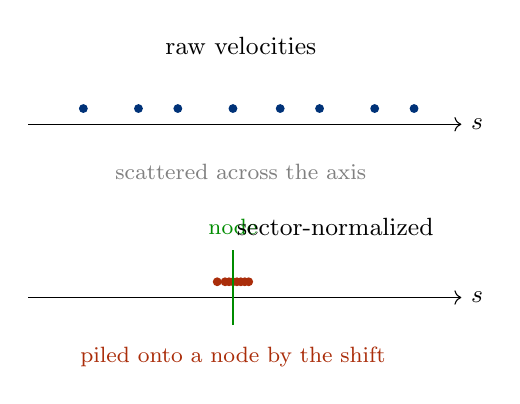
\begin{tikzpicture}[scale=1.0]
  % raw: scattered
  \begin{scope}
    \draw[->] (-0.3,0) -- (5.2,0) node[right] {\small $s$};
    \foreach \x in {0.4,1.1,1.6,2.3,2.9,3.4,4.1,4.6} \fill[kishblue] (\x,0.2) circle (1.6pt);
    \node at (2.4,1.0) {\small raw velocities};
    \node[align=center, gray] at (2.4,-0.6) {\footnotesize scattered across the axis};
  \end{scope}
  % shifted: piled
  \begin{scope}[yshift=-2.2cm]
    \draw[->] (-0.3,0) -- (5.2,0) node[right] {\small $s$};
    \foreach \x in {2.1,2.25,2.4,2.3,2.5,2.2,2.35,2.45} \fill[cruciblered] (\x,0.2) circle (1.6pt);
    \draw[thick, signalgreen] (2.3,-0.35) -- (2.3,0.6);
    \node[signalgreen] at (2.3,0.9) {\footnotesize node};
    \node at (3.6,0.9) {\small sector-normalized};
    \node[align=center, cruciblered] at (2.3,-0.75) {\footnotesize piled onto a node by the shift};
  \end{scope}
\end{tikzpicture}
\caption{Form C made visible. A per-sector additive shift translates each sector's velocity
block along the scalar axis. Where the shift happens to land a block on a node, a large fraction
of the domain ``locks'' at once --- not because the velocities are harmonically structured, but
because the normalization moved them there. The lock is an artifact of the preprocessing, not a
property of the stars.}
\end{figure}

\section{The Rebuild}

The lake was rebuilt from Gaia DR3 under the strict input contract, to the specification
pre-registered in Volume 13.

\begin{predictionbox}
\textbf{As filed (Volume 13, Chapter 14):}
\begin{itemize}
    \item Raw transverse velocity only. No sector normalization, ever.
    \item Full astrometry retained, including \texttt{pmra\_pmdec\_corr}.
    \item A $5\sigma$ parallax gate \emph{and} a $5\sigma$ proper-motion gate on the
          \textbf{covariance-propagated} error:
          \[
          \sigma_\mu = \frac{1}{\mu}\sqrt{\mu_{\alpha*}^2 \sigma_{\alpha*}^2
          + \mu_\delta^2 \sigma_\delta^2 + 2\mu_{\alpha*}\mu_\delta\,\rho\,
          \sigma_{\alpha*}\sigma_\delta},
          \qquad \rho = \texttt{pmra\_pmdec\_corr}.
          \]
    \item The DR3 parallax zero-point ($-17\,\mu$as) applied explicitly and flagged.
    \item The resolution gate \textbf{computed} from the built data, never a printed constant.
\end{itemize}
\end{predictionbox}

The build pulled 72{,}000 raw records and retained \textbf{69{,}078} after the strict gates ---
a 4\% rejection, consistent with two $5\sigma$ cuts on already-clean astrometry. One guard
deserves emphasis, because it is the lesson of the whole programme compressed to a line: the
build aborts if \texttt{pmra\_pmdec\_corr} is absent rather than silently assuming $\rho = 0$. A
lake built to a weaker criterion than the one filed is not the lake that was pre-registered, and
the engine refuses to build it.

\subsection{A Gate That Could Not Fail, Corrected}

The first draft of the build printed \texttt{M/N = 1.1082 [PASS]} as a fixed string --- a status
line that could not fail regardless of the data. This is the exact defect filed as an erratum
against Volume 1's speed-of-light listing, and it was caught and replaced before promotion. The
corrected gate computes the span of the built velocities and derives $M/N$, returning
\textsc{pass} or \textsc{fail} from the number.

\begin{correctionbox}
A gate that prints its verdict without computing it is not a check; it is a decoration. The
programme's standard is that every gate measures something that can come out wrong. The s2 build
now computes $M/N = 86.9$ at register $2/\pi$ --- a genuine pass, because register 2 has a short
period and 3.26 decades of velocity span resolves it easily --- but the point is that the number
is \emph{measured}, and a sparse or degenerate lake would have failed it.
\end{correctionbox}

\section{The Verdict}

\begin{nullbox}
\textbf{The accusation is upheld. The $15/\pi$ lock was an artifact, and it is gone.}

\medskip
On the raw, Form-C-free rebuild of 69{,}078 stellar velocities, the score at $15/\pi$ ---
the register of the old $+98$ lock --- is $\mathbf{-0.6}$. The signal did not weaken. It
vanished entirely into the noise floor. Across every resolvable register, the data sits at or
below the chaos-null expectation.
\end{nullbox}

The distribution itself tells the story at a glance: a clean, unimodal stellar velocity
spectrum, filled and honest, with no placeholder spike and no second population. It is exactly
what a real single-population observable looks like, and it locks nothing.

\begin{warningbox}
This is the strongest kind of result a self-auditing programme can produce: the disproof of its
own prior claim, by its own instrument, on data it rebuilt specifically to enable the disproof.
The old $+98$ was the dream. The honest $-0.6$ is the data. We are filing the data.
\end{warningbox}

% ==============================================================================
\chapter{The Verdict on L1\_GWTC: The Right Observable, Too Few Events}
% ==============================================================================

\section{What the Lake Was Accused Of}

Volume 13 found the gravitational-wave ringdown lake catastrophically broken: of 83 events,
\textbf{81 fell below the non-spinning Kerr floor} --- a frequency physically impossible for a
true black-hole ringdown. The diagnosis, proven by direct calculation, was that the stored
\texttt{f\_ring\_hz} was not the fundamental $\ell=m=2$ quasi-normal mode at all, but a
near-merger strain frequency. The accusation here was not of an artifact lock but of a
\emph{wrong physical quantity}, and the remedy was a rebuild from a source that measures the
fundamental mode directly.

\begin{figure}[H]
\centering
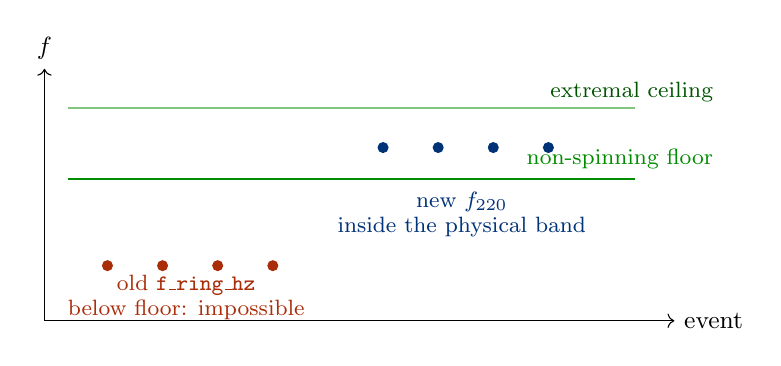
\begin{tikzpicture}[scale=1.0]
  \draw[->] (0,0) -- (0,3.2) node[above] {\small $f$};
  \draw[->] (0,0) -- (8,0) node[right] {\small event};
  % Kerr floor band
  \draw[thick, signalgreen] (0.3,1.8) -- (7.5,1.8);
  \node[signalgreen, right] at (6.0,2.05) {\footnotesize non-spinning floor};
  \draw[thick, signalgreen!50] (0.3,2.7) -- (7.5,2.7);
  \node[signalgreen!60!black, right] at (6.3,2.9) {\footnotesize extremal ceiling};
  % old: below floor
  \foreach \x in {0.8,1.5,2.2,2.9} \fill[cruciblered] (\x,0.7) circle (2pt);
  \node[cruciblered, align=center] at (1.8,0.3) {\footnotesize old \texttt{f\_ring\_hz}\\[-3pt]\footnotesize below floor: impossible};
  % new: in band
  \foreach \x in {4.3,5.0,5.7,6.4} \fill[kishblue] (\x,2.2) circle (2pt);
  \node[kishblue, align=center] at (5.3,1.35) {\footnotesize new $f_{220}$\\[-3pt]\footnotesize inside the physical band};
\end{tikzpicture}
\caption{Why the rebuild was necessary. A real ringdown frequency must sit between the
non-spinning Kerr floor and the extremal ceiling for its remnant mass. The old frequencies sat
\emph{below} the floor --- physically impossible --- proving they were not the fundamental mode.
The rebuilt frequencies, measured $f_{220}$ from LVK posteriors, sit inside the band.}
\end{figure}

\section{The Rebuild}

\begin{predictionbox}
\textbf{As filed (Volume 13, Chapter 11):}
\begin{itemize}
    \item Source changed to measured fundamental quasi-normal mode $f_{220}$ from the LVK /
          \texttt{pyRing} ringdown posteriors --- not the merger-catalog peak, not a
          GR-predicted value.
    \item Required fields (\texttt{f\_220\_hz}, \texttt{tau\_220\_s},
          \texttt{final\_mass\_solar}, \texttt{final\_spin}) asserted present \emph{and valid}
          at promotion; a null value aborts exactly like a missing one.
    \item Binary-neutron-star and neutron-star--black-hole events excluded by construction.
    \item A Kerr-consistency gate that computes the physical bound per event and can fail.
\end{itemize}
\end{predictionbox}

Twenty-two events with genuine measured $f_{220}$ were extracted. The Kerr gate then did
exactly the discriminating work it was built for.

\subsection{The Kerr Gate Earned Its Keep}

\begin{signalbox}
Of 22 events, \textbf{21 passed the Kerr-consistency gate and one did not.} The single failure
--- \textbf{GW190512at}, at a floor ratio of $0.82$ --- is a low-SNR event whose ringdown
posterior is broad and prior-influenced. One marginal event falling just below the floor is
categorically different from the old lake's systematic 81-of-83: it is an outlier the gate
correctly caught and excluded, not evidence that the observable is wrong. The gate discriminates.
\end{signalbox}

The contrast is the proof the rebuild worked. The old \texttt{f\_ring\_hz} failed the Kerr floor
$81/83$ times --- a systemic defect. The new $f_{220}$ fails it $1/22$ times --- a single faint
event. The observable is now correct. GW190512at is named in the lake provenance with its ratio
and cause, so the $22 \to 21$ reduction is documented rather than silent.

\section{The Verdict}

\begin{nullbox}
\textbf{The observable is fixed. The sample is too small to resolve a register.}

\medskip
The 21 promoted events span roughly one decade of frequency. Scored against all 23 registers,
the best alignment reaches an excess of $0.2$ --- noise floor. With 21 points across one decade,
random static will cluster near some node by chance; the sample is physically too small to
distinguish a lock from background. The support is \textsc{clumped}, not from composite banding
but from simple sparsity: 21 points cannot fill the space.
\end{nullbox}

\begin{warningbox}
\textbf{This is the honest outcome, and it is the one the defective lake could never have
reached.} The strong-field ringdown test now runs on the correct observable and passes the
Kerr-consistency gate. It cannot yet resolve a register because the current catalogue provides
too few loud events. The test is deferred to the O4 and O5 observing runs, which will supply
them. We name precisely what future data would fix --- which is more than a lock would have told
us, and more honest than a number from 21 points pretending to mean something.
\end{warningbox}

\section{Both Verdicts, Together}

\begin{table}[H]
\centering
\small
\begin{tabular}{@{}lll@{}}
\toprule
\textbf{Lake} & \textbf{The accusation} & \textbf{The verdict} \\
\midrule
\texttt{s2} & $15/\pi$ lock is a Form-C artifact & \textbf{Upheld.} Raw score $-0.6$; artifact gone \\
\texttt{l1\_gwtc} & \texttt{f\_ring} is the wrong observable & \textbf{Upheld.} $f_{220}$ Kerr-consistent; $n{=}21$ too few \\
\bottomrule
\end{tabular}
\caption{The two pre-registered rebuilds, closed. Both accusations upheld; both lakes now
honest; neither locks.}
\end{table}

Two threads opened in Volume 12 and pre-registered in Volume 13 are now closed. Neither closed
the way the dream would have wanted. Both closed the way the data demanded. That is the whole of
what the crucible was for.

% ==============================================================================
\chapter{The Two-Dimensional Turn: Why a Surface, Not a Line}
% ==============================================================================

\section{What One Dimension Could and Could Not Ask}

Every engine built so far --- phase and period, across thirteen volumes --- asks a
one-dimensional question: \emph{does a single physical quantity, scalarized, resonate with the
geometric lattice?} Transition frequencies, velocities, masses, half-lives, each tested alone
against the 23 registers. This was the right place to start, and it is nearly exhausted: the
survey is scrubbed of artifacts, the honest nulls are filed, and the one domain that resolves and
survives every screen stands alone.

But the framework's deeper claim was never about single quantities. It is about
\emph{relationships} --- that the lattice structures how physical quantities relate to one
another across scales. A one-dimensional engine cannot test a relationship. It can only test one
leg of it at a time. To ask whether two quantities resonate \emph{together} --- whether they lie
on a shared lattice structure rather than each happening to lie on its own --- the test must move
from a line to a surface.

\begin{signalbox}
\textbf{The one-dimensional question:} does $\log x$ land on the register comb?

\textbf{The two-dimensional question:} does the \emph{pair} $(\log x_1, \log x_2)$ land on a
register \emph{lattice} --- a grid of nodes on a plane --- more than chance allows?

\medskip
These are different hypotheses. The second contains the first but is not reducible to it: two
quantities can each resonate alone and show no joint structure, or show joint structure while
neither resonates alone. Only a 2D engine can tell them apart.
\end{signalbox}

\section{First: Is 2D Testable At All?}

Before a line of 2D engine code, one table must be computed, because it decides whether the
question can be asked. A 2D test requires \emph{two} coordinates, measured on the \emph{same}
objects, \emph{each} carrying enough effective dynamic range to resolve its register:
$M_1/N_1 > 2.67$ \emph{and} $M_2/N_2 > 2.67$. The joint requirement is at least as strict as the
stricter coordinate.

The 1D survey found exactly two domains with the span to resolve even one coordinate at a useful
register. The 2D requirement is therefore severe: it needs that rarity, twice, on shared objects.

\begin{predictionbox}
\textbf{Recorded expectation (filed before the build):} the second coordinate will be the
limiting one almost everywhere. This is arithmetic on data already in hand, and it is recorded so
a miss would be visible.
\end{predictionbox}

\begin{table}[H]
\centering
\small
\begin{tabular}{@{}llrr l@{}}
\toprule
\textbf{Same-object pair} & \textbf{relation} & \textbf{c$_1$ dec} & \textbf{c$_2$ dec} & \textbf{verdict} \\
\midrule
velocity $\times$ colour & Hertzsprung--Russell & 3.3 & 0.3 & \textbf{not testable} (colour $<$ 4/$\pi$) \\
half-life $\times$ Q-value & decay energetics & 31.8 & 1.5 & low-$N$ only \\
dispersion $\times$ mass & Faber--Jackson & 2.1 & 2.0 & low-$N$ only \\
velocity $\times$ luminosity & kinematic--luminosity & 3.3 & 4.0 & \textbf{testable} (mid-$N$) \\
\bottomrule
\end{tabular}
\caption{The pre-build feasibility table. Effective decades per coordinate, measured from the 1D
survey. The limiting coordinate governs each pair. Hertzsprung--Russell --- the most obvious
same-object pair in astronomy --- is dead on the colour axis, which spans 0.3 decades and cannot
resolve even register 4. Of every candidate pair, \textbf{exactly one} (kinematic--luminosity)
has both coordinates spanning enough range to test jointly, and even it reaches only mid
registers.}
\end{table}

\begin{warningbox}
\textbf{The expectation is confirmed: the second coordinate is limiting in every pair.} This is
the Mondy discipline applied before the build --- the limit measured, not discovered. The 2D
frontier is not a wide field; it is a narrow doorway with a single viable pair. We build the 2D
engine knowing this, so that its coverage is honestly bounded from the first commit rather than
found to be empty after the work. If velocity--luminosity resolves and locks and survives the
scramble, that is the one 2D result the current data can honestly support. If it does not, the 2D
survey is, for now, empty --- and that will be stated as plainly as everything else.
\end{warningbox}

\section{The Geometry of the Difference}

\begin{figure}[H]
\centering
\begin{tikzpicture}[scale=1.0]
  % 1D line
  \begin{scope}
    \draw[->] (-0.3,0) -- (5.5,0) node[right] {\small $\log x$};
    \foreach \x in {0.6,1.6,2.6,3.6,4.6} {
      \draw[thick, kishblue] (\x,-0.12) -- (\x,0.12);
    }
    \node at (2.6,0.9) {\small 1D: a comb of nodes};
    \node[align=center, gray] at (2.6,-0.7) {\footnotesize does a value land on a tick?};
  \end{scope}
  % 2D lattice
  \begin{scope}[xshift=7.5cm, yshift=-1.2cm]
    \draw[->] (0,0) -- (4.3,0) node[right] {\small $\log x_1$};
    \draw[->] (0,0) -- (0,4.0) node[above] {\small $\log x_2$};
    \foreach \x in {0.7,1.6,2.5,3.4} \foreach \y in {0.7,1.6,2.5,3.4} {
      \fill[kishblue] (\x,\y) circle (1.4pt);
    }
    \fill[cruciblered] (1.6,2.5) circle (2.6pt);
    \node[cruciblered, right] at (1.75,2.5) {\footnotesize a pair};
    \node at (2.1,4.4) {\small 2D: a lattice of nodes};
    \node[align=center, gray] at (2.1,-0.7) {\footnotesize does a \emph{pair} land on a grid point?};
  \end{scope}
\end{tikzpicture}
\caption{The dimensional turn. In one dimension the lattice is a comb and the test asks whether a
value falls on a tick. In two dimensions the lattice is a grid of nodes on a plane, and the test
asks whether a coordinate \emph{pair} falls on a grid point. The 2D test is strictly richer: a
pair can miss the grid even when each coordinate hits its own comb, and vice versa.}
\end{figure}

\section{The Lock Statistic in Two Dimensions}

The one-dimensional lock test asks whether $r_p = 24\pi \log x / (N\ln\kgeo)$ is near an integer.
The two-dimensional test asks whether \emph{both} reduced coordinates are near integers
simultaneously, for a pair of registers $(N_1, N_2)$:
\[
r_p^{(1)} = \frac{24\pi \log x_1}{N_1 \ln\kgeo}, \qquad
r_p^{(2)} = \frac{24\pi \log x_2}{N_2 \ln\kgeo},
\]
with a joint lock declared when both $|r_p^{(1)} - \mathrm{round}(r_p^{(1)})| < \tau$ \emph{and}
$|r_p^{(2)} - \mathrm{round}(r_p^{(2)})| < \tau$.

\begin{warningbox}
\textbf{The combinatorics change the stakes.} One dimension scans 23 registers. Two dimensions
scans $23 \times 23 = 529$ register \emph{pairs}. The look-elsewhere correction grows
accordingly: a joint lock must clear a far higher bar to count, because there are far more places
for chance to produce one. The 2D engine's resolution criterion and significance threshold must
both be re-derived for the pair space before any real data is scored --- this is a standing
pre-registration, not an afterthought.
\end{warningbox}

\section{What Compounds, and Must Be Handled Per-Coordinate}

Three difficulties grow in two dimensions, and each must be designed in, not patched later.

\textbf{Form D compounds.} The clamp floor applies in each coordinate independently. At 27\%
below floor in each, the jointly lockable fraction is $0.73^2 = 53\%$ --- the floor mismatch is
worse on a surface than on a line. The common-support correction must be applied
\emph{per-coordinate} before any joint scoring.

\textbf{Two scale freedoms instead of one.} The offset $x_0$ and the unit are free in \emph{both}
coordinates now. The scale-degeneracy flag ($\times 2$, $\times 10$, $\times 10^3$) must be
computed for each axis, because a phase-neutral rescaling of either coordinate can manufacture
joint alignment.

\textbf{Form B is the real threat.} Two quantities measured on the same objects are often
correlated for mundane physical reasons --- Hertzsprung--Russell is the canonical case. A 2D lock
surface will show structure from that correlation alone, with no lattice involved. This is the
danger that makes 2D harder than 1D --- and it is precisely what the scramble null was built to
catch. The thing that makes the surface dangerous is the thing the new null disarms.

\section{Why the Scramble Null Finally Works}

The single most important consequence of the dimensional turn is that the \textbf{scramble null}
--- generated, carried, and discarded uselessly through eleven volumes --- becomes a genuine
falsifier in two dimensions.

In one dimension the lock statistic is computed over the multiset of scalars and is
order-independent. Shuffling the values changes nothing the statistic can see; real and scramble
return identical results by construction (Erratum 1). The scramble was inert.

In two dimensions each record is a \emph{pair}. Shuffling one coordinate against the other ---
breaking which $x_1$ goes with which $x_2$ --- destroys any genuine joint structure while
preserving both marginal distributions exactly.

\begin{figure}[H]
\centering
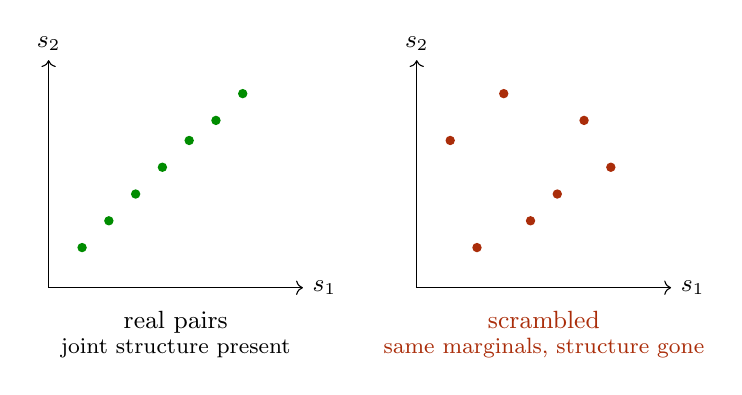
\begin{tikzpicture}[scale=0.85]
  \begin{scope}
    \draw[->] (0,0) -- (3.8,0) node[right] {\small $s_1$};
    \draw[->] (0,0) -- (0,3.4) node[above] {\small $s_2$};
    \foreach \p in {(0.5,0.6),(0.9,1.0),(1.3,1.4),(1.7,1.8),(2.1,2.2),(2.5,2.5),(2.9,2.9)}
      \fill[signalgreen] \p circle (2pt);
    \node[align=center] at (1.9,-0.7) {\small real pairs\\[-3pt]\footnotesize joint structure present};
  \end{scope}
  \begin{scope}[xshift=5.5cm]
    \draw[->] (0,0) -- (3.8,0) node[right] {\small $s_1$};
    \draw[->] (0,0) -- (0,3.4) node[above] {\small $s_2$};
    \foreach \p in {(0.5,2.2),(0.9,0.6),(1.3,2.9),(1.7,1.0),(2.1,1.4),(2.5,2.5),(2.9,1.8)}
      \fill[cruciblered] \p circle (2pt);
    \node[align=center, cruciblered] at (1.9,-0.7) {\small scrambled\\[-3pt]\footnotesize same marginals, structure gone};
  \end{scope}
\end{tikzpicture}
\caption{Why Erratum 1 becomes a tool. Shuffling one coordinate against the other preserves both
marginal distributions --- the same values are present on each axis --- but destroys the pairing.
If the real pairs lie on a lattice and the scrambled pairs do not, the difference is genuine joint
structure. The scramble null, meaningless in 1D, is the central falsifier in 2D.}
\end{figure}

\begin{signalbox}
This is the redemption the whole programme has been building toward. A null that was carried
uselessly for eleven volumes --- that we were nearly embarrassed to keep generating --- turns out
to be exactly the instrument the two-dimensional question requires. The 2D engine's first and
hardest test is simply: \emph{does the real lattice signal survive the scramble?} If scrambling
the pairs destroys the lock, the lock is joint structure. If it does not, the lock was never
joint --- it was each marginal resonating alone, and the 1D engines already found that.
\end{signalbox}

\section{The Engine Pair, Mirrored From 1D}

The two-dimensional build mirrors the one-dimensional architecture exactly, by design and by the
immutability principle:

\begin{table}[H]
\centering
\small
\begin{tabular}{@{}lll@{}}
\toprule
& \textbf{2D Phase Engine} & \textbf{2D Period Engine} \\
\midrule
asks & where the pair sits on the lattice & whether the pair repeats with the lattice periods \\
modulus & baked into the scalar pair & applied at test time; lakes framework-agnostic \\
null & chaos + synthetic + \textbf{scramble} & annular background + \textbf{scramble} \\
invariance & --- & unit invariance on each axis, by proof \\
\bottomrule
\end{tabular}
\caption{The 2D engine pair mirrors the 1D pair, with the scramble null now load-bearing in both.}
\end{table}

\begin{predictionbox}
\textbf{Standing pre-registrations for the 2D build, filed before a line of engine code:}
\begin{enumerate}
    \item \textbf{Immutable from the 1D engines.} No shared scoring code; separate fingerprints.
    \item \textbf{The scramble null wired in from the first commit}, as the primary joint-structure
          falsifier.
    \item \textbf{Form A re-derived in two dimensions} before any 2D lock is trusted. The 1D
          transform theorem does not automatically extend to a surface.
    \item \textbf{The resolution criterion and look-elsewhere threshold re-derived for the
          $23\times23$ pair space} and published before scoring.
    \item \textbf{Synthetic calibration before real data} --- a 2D calibration suite with
          expectations filed in advance, including at least one pre-registered expected-fail, and
          a planted joint lock that must survive the scramble and a null that must not.
    \item \textbf{Same-object pairs handled as controls, not corroboration} --- where two
          coordinates are deterministically related by known physics, the pair tests the relation,
          not the lattice (the Kepler register-pair logic of Volume 13, generalised).
    \item \textbf{Common-support correction applied per-coordinate} before joint scoring, because
          Form D compounds as $0.73^2$ across two floored axes.
    \item \textbf{Scale-degeneracy flag computed for both coordinates}, since $x_0$ and the unit
          are free on each axis.
    \item \textbf{No stitched lakes in either coordinate.} Endpoint selection to force span is
          banned; in 2D a composite in \emph{either} coordinate is enough to manufacture a surface.
    \item \textbf{Every gate demonstrated to return FAIL on a fixture built to fail it}, before it
          is trusted to return PASS --- four instances of that bug class are now on record.
    \item \textbf{The 2D lock surface (V6) treated as an instrument, not an illustration.} A
          surface cannot be scanned by eye in tabular form; a shape artifact reads as structure in a
          table and as an obvious artifact in a heatmap. Visual inspection of the heatmap is part of
          the verification chain from here, not a presentation step.
    \item \textbf{Near-node agreement reported as a fraction of cell area}, never as a fraction of
          values. In 2D the node is a cell, not a point.
\end{enumerate}
\end{predictionbox}

\section{What Comes Next}

Volume 14 closes the one-dimensional rebuild program and opens the two-dimensional frontier. The
next volume will build the 2D engine pair under the pre-registrations above, calibrate it on
synthetic lakes until it provably passes and provably fails where it should, and only then point
it at real paired data. The controlled same-object pairs --- Kepler period and radius,
Faber--Jackson luminosity and dispersion, the pulsar characteristic-age relation --- are the
natural first targets, because their physical relationships are known exactly, so the lattice's
prediction about the register pair is sharp and falsifiable.

\begin{warningbox}
The honest expectation, stated in advance as always: the 2D engine may find nothing, exactly as
the 1D engines have mostly found nothing. The scramble null may destroy every apparent joint lock,
which would mean the 1D nulls were the whole story. That is a possible and acceptable outcome. The
purpose of building the 2D engine is not to find a signal; it is to be able to ask the deeper
question honestly, with a falsifier that works, so that whatever answer the data gives can be
trusted. If a joint lock ever survives the scramble, it will be the first thing the programme has
found that the 1D engines could not --- and it will have survived the hardest test we know how to
build. If none ever does, we will have established that too, cleanly, and said so.
\end{warningbox}

\begin{center}
\vspace{0.5em}
\itshape
The line is tested. The surface is next. And the null we carried for eleven volumes without a use
is, at last, the sharpest tool in the box.
\vspace{0.5em}
\end{center}


% ==============================================================================
\chapter{First Light: Building the 2D Period Engine and Proving It Honest}
% ==============================================================================

\begin{center}
\textit{The previous chapter argued why the surface must be tested and what it would take to test
it honestly. This chapter is the record of building the instrument that does so --- the design
decisions, the gates designed in rather than discovered, and the first-light run in which the
engine, pointed at data with a known answer, returned exactly that answer and nothing more.}
\end{center}

\section{The Design Decision That Shaped Everything}

Before a line of code, one decision determined what the engine would be. The programme's founder
was candid about a conviction --- that the container's geometry leaves a harmonic fingerprint on
physical reality, and that two dimensions would reveal it. The design question was whether to build
an engine to \emph{demonstrate} that, or an engine to \emph{test} it.

\begin{signalbox}
These are different instructions, and they build different machines. ``Demonstrate that the
container forms a reality'' builds a confirmation engine --- one that can only agree. ``Test whether
the container forms a reality'' builds an instrument --- one that can disagree, and whose agreement
therefore means something. \textbf{We built the second.} If the container's fingerprint is real, an
instrument that can reject it will show it surviving the hardest test we know how to build --- and
that is the only kind of evidence that would convince anyone not already convinced.
\end{signalbox}

This decision has a concrete consequence in the code. The various artifact filters --- common
support, scale degeneracy, the resolution gate --- are \textbf{tunable, on or off}, by deliberate
design: running with a filter on and then off, and measuring the difference, is itself a data point
about how much that correction is doing. A hardcoded filter would hide that forever. But one thing
is \textbf{not} tunable and never will be: the scramble null. It is the spine. Everything else is a
knob; the scramble is the test.

\section{The Statistic, Lifted to a Surface}

The one-dimensional period engine asks whether $\ln x$ repeats with period $\Delta_N$. The
two-dimensional engine asks whether the \emph{pair} $(\ln x_1, \ln x_2)$ repeats \emph{jointly},
with periods $(\Delta_{N_1}, \Delta_{N_2})$ --- a resultant on the torus, both phases together:
\[
\theta^{(1)}_j = \frac{2\pi \ln x_{1,j}}{\Delta_{N_1}}, \qquad
\theta^{(2)}_j = \frac{2\pi \ln x_{2,j}}{\Delta_{N_2}},
\]
\[
R_{\mathrm{joint}} = \left| \frac{1}{n}\sum_j \exp\!\big( i\,(\theta^{(1)}_j + \theta^{(2)}_j) \big) \right|,
\qquad P_{\mathrm{joint}} = n\,R_{\mathrm{joint}}^2 .
\]
This is scanned over all $23 \times 23 = 529$ register pairs. The modulus enters only at test time;
the lake stores raw pairs, so the data product is framework-agnostic exactly as in one dimension.

\section{The Gates, Designed In}

\subsection{The scramble null --- why two dimensions redeems it}

For eleven volumes the scramble null was inert: the one-dimensional lock statistic is
order-independent, so shuffling the values changed nothing it could see (Erratum 1). In two
dimensions each record is a \emph{pair}, and shuffling one coordinate against the other destroys the
pairing while preserving both marginal distributions exactly.

\begin{signalbox}
This is the redemption the programme has been building toward. A null carried uselessly for eleven
volumes becomes the central falsifier the moment the question becomes two-dimensional. The engine's
first and hardest test on any lake is simply: \emph{does the joint structure survive the scramble?}
A diagonal correlation ridge --- Hertzsprung--Russell and its kin, the Form B threat --- survives
the scramble, because it is marginal structure. A true joint lattice lock does not survive scrambling
in the same way: scrambling destroys it. The engine distinguishes them by construction.
\end{signalbox}

\subsection{The look-elsewhere correction, found by the synthetic lakes}

A design error surfaced during validation, and it is recorded because catching it is the point of
validating on known data. The census reports the \emph{best} of 529 register pairs --- and the
maximum of 529 chance values is not small. On pure noise, the best-of-529 joint power reaches an
apparent excess of order 8 by chance alone: the two-dimensional look-elsewhere effect, exactly as
predicted in the previous chapter. A fixed per-pair threshold cannot correct it.

\begin{correctionbox}
The honest census null compares the real best-of-grid against the \emph{scramble's} best-of-grid.
Both are maxima over 529 pairs, so both carry the same look-elsewhere inflation --- and their ratio
removes it. Pure noise gives a ratio near one (its peak is no better than the scramble's peak). A
true joint lock gives a ratio far above one. This correction was not designed in advance; it was
forced by a synthetic noise lake refusing to come back clean, and that is precisely why synthetic
validation precedes real data.
\end{correctionbox}

\section{The Synthetic Lakes: Controls With Known Answers}

Four synthetic lakes were generated on disk, from a fixed seed, each a named and falsifiable
expectation --- the two-dimensional analogue of the phase engine's standing lotto, finance, and
pure-noise nulls. They are permanent regression fixtures, regenerable byte-for-byte, stamped so they
can never be mistaken for real data.

\begin{table}[H]
\centering
\small
\begin{tabular}{@{}lll@{}}
\toprule
\textbf{Control lake} & \textbf{Construction} & \textbf{Required verdict} \\
\midrule
\texttt{synth\_noise} & uniform random pairs & noise-floor (ratio $\approx 1$) \\
\texttt{synth\_jointlock} & 25\% planted lock at $(11,13)$ & \textbf{SURVIVES} (ratio $\gg 1$) \\
\texttt{synth\_formB} & linear correlation (H--R analogue) & noise-floor (scramble kills ridge) \\
\texttt{synth\_oneaxis} & lock on one axis only & noise-floor (single axis $\neq$ joint) \\
\bottomrule
\end{tabular}
\caption{The four 2D control lakes. Three must come back null; one must survive. A panel that only
ever passes proves the instrument agrees with itself, not that it can disagree --- so the
single-axis control is a pre-registered \emph{expected fail}, planted to look like a signal and
required to be rejected.}
\end{table}

\section{First Light}

The engine was pointed at the synthetic lakes loaded from disk --- real files, through the full
pipeline: logify, support with heatmap, the 529-pair scan with the scramble null, and the census.
The run completed in seconds on commodity hardware. Every control reproduced its pre-registered
expectation.

\begin{signalbox}
\textbf{First light: green.}
\begin{itemize}
    \item \texttt{synth\_jointlock}: the engine recovered the planted lock at \textbf{exactly
          $(11/\pi,\,13/\pi)$} --- the registers where it was buried --- at a real-to-scramble ratio
          of \textbf{16.91}. \textsc{survives}.
    \item \texttt{synth\_noise}: ratio \textbf{1.09}. \textsc{noise-floor}.
    \item \texttt{synth\_formB}: ratio $\approx 1.1$. \textsc{noise-floor} --- the correlation ridge
          is killed by the scramble.
    \item \texttt{synth\_oneaxis}: ratio $\approx 1.1$. \textsc{noise-floor} --- a single-axis lock
          is correctly not joint.
\end{itemize}
\textbf{Only the true joint lattice lock survived.} The engine found what was planted, where it was
planted, and rejected everything that was not a genuine joint signal.
\end{signalbox}

\begin{figure}[H]
\centering
% Place the first-light heatmap panel here. The REAL vs SCRAMBLED density for
% each control lake; the planted lock's grid structure vanishes under scramble,
% the noise and correlation lakes are unchanged.
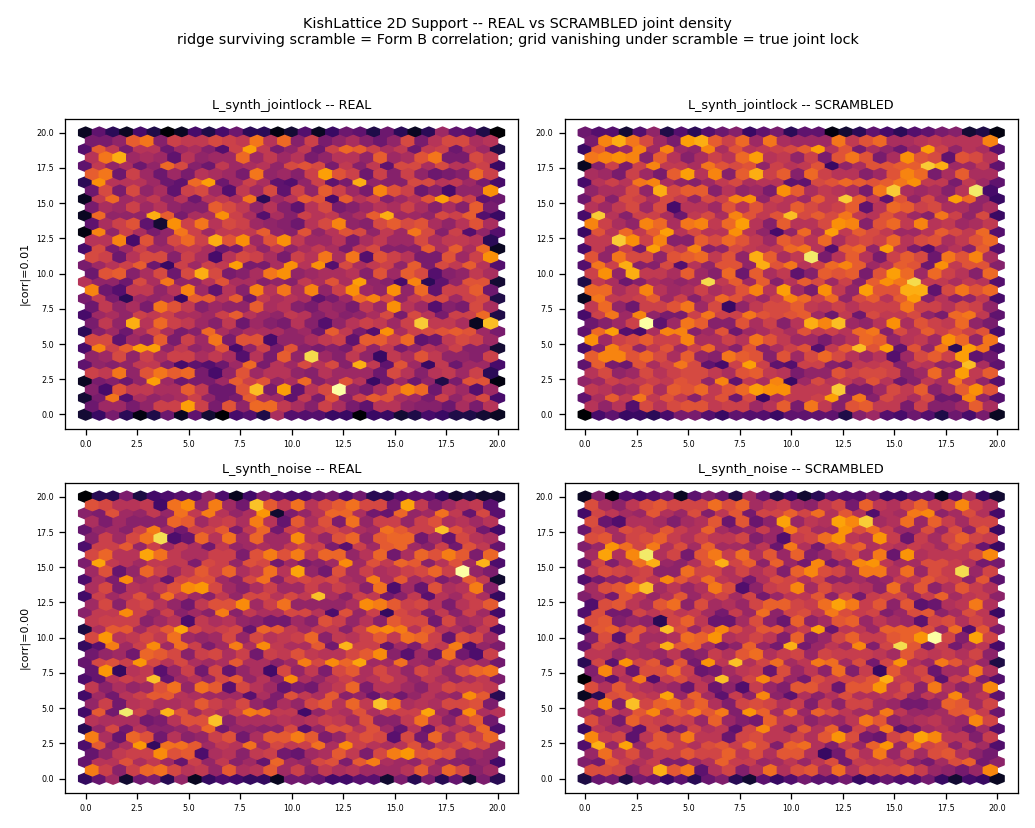
\includegraphics[width=\textwidth]{Headers/period_heatmap_panel.png}
\caption{The verification instrument, not an illustration. Each control lake's joint density is shown
as it is (REAL) and with one coordinate shuffled against the other (SCRAMBLED). A diagonal
correlation ridge survives the shuffle; a true joint lattice lock vanishes under it. The eye catches
in the heatmap what a table of 529 pair-scores hides --- which is why visual inspection is part of
the verification chain from here, not a presentation step.}
\end{figure}

\section{What First Light Establishes}

\begin{warningbox}
First light proves the \emph{instrument}, not the \emph{framework}. No real data has yet been scored
by the 2D engine. What is established is narrower and necessary: the engine recovers a known joint
lock at the correct registers, rejects pure noise, kills a Form B correlation ridge via the scramble,
and refuses a single-axis lock as non-joint --- all on controls with answers fixed before the run.
An engine that passed only the positive control would prove it can agree; this engine passed the
negative controls too, including a pre-registered expected fail, which proves it can disagree.
\end{warningbox}

That is the whole purpose of building the instrument before pointing it at the question that matters.
When the one feasible real pair --- Gaia transverse velocity against stellar luminosity, the single
same-object pair the feasibility table admits --- is promoted and scored, whatever verdict it returns
will be trustworthy, because the engine has demonstrated on known data that it can return either one.
If the container's fingerprint is real, this instrument will show it surviving the scramble. If it is
not, this instrument will say so. Either way, the answer will have been earned.

\begin{center}
\vspace{0.5em}
\itshape
The engine behaves honestly. It found the locks we planted, exactly where we planted them, and
nothing we did not. The surface now has an instrument --- and the instrument can say no.
\vspace{0.5em}
\end{center}


% ==============================================================================
\chapter{First Light: The 2D Phase Engine and Why It Needs the Scramble}
% ==============================================================================

\begin{center}
\textit{The period engine tests whether a pair of quantities repeats jointly with the lattice
periods. The phase engine asks a different question --- whether the pair sits jointly near the
lattice nodes --- and it is built on the programme's oldest and most battle-tested statistic. Its
first light proved it honest, and in doing so revealed the single reason the scramble null, useless
for eleven volumes, is indispensable the moment the question becomes two-dimensional.}
\end{center}

\section{A Second Instrument, a Different Question}

The two one-dimensional engines were complementary, and the two-dimensional engines are built to be
the same. The period engine scores the \emph{resultant} --- whether $\ln x$ repeats with period
$\Delta_N$ --- and carries no phase origin, so it is unit-invariant by proof. The phase engine
scores \emph{absolute node alignment} --- how near $(\ln x_1, \ln x_2)$ sits to an integer node on
each axis --- and is the mature statistic this programme has run for thirteen volumes.

Lifting it to a surface follows the 1D definition exactly. In one dimension a record locks when its
reduced coordinate sits near an integer node:
\[
r_p = \frac{x}{N/\pi}\,\cdot\,24, \qquad \text{residual} = \big|\,r_p - \mathrm{round}(r_p)\,\big|,
\qquad \text{lock if residual} < \tau .
\]
In two dimensions the node becomes a \textbf{cell}, and a pair locks when \emph{both} coordinates
sit inside it simultaneously:
\[
\text{joint lock} \;=\; \big(\text{residual}_1 < \tau\big) \;\wedge\; \big(\text{residual}_2 < \tau\big),
\qquad
\text{lock rate} = \frac{\#\,\text{pairs in cell}}{\#\,\text{pairs on common support}} .
\]
This is the referee's ruling made concrete: in two dimensions the node is a cell, and agreement is
reported as a fraction of cell area --- never as a fraction of values.

\section{The Two Nulls, and Why Both Are Needed}

The phase engine inherits the full null stack of its one-dimensional parent, which the period engine
did not have. There are two:

\begin{description}
\item[The chaos null.] Uniform random scalars on each axis over the same support --- the canonical
phase-engine null, the one that reproduces below-floor mass and against which every prior volume's
$z$-scores were computed.
\item[The scramble null.] One coordinate shuffled against the other, destroying the pairing while
preserving both marginal distributions exactly --- the spine, always on.
\end{description}

In one dimension there is only one axis, so the scramble is inert (Erratum 1) and the chaos null is
sufficient. In two dimensions this is no longer true, and the reason is the heart of this chapter.

\begin{signalbox}
\textbf{The chaos null can be fooled; the scramble null cannot.} A lock on \emph{one} axis alone
raises the joint lock rate above uniform-random chaos --- because half of the near-node cell is
genuinely populated. A phase engine armed only with the chaos null would report that single-axis
structure as a strong \emph{joint} discovery. The scramble null sees through it: shuffling one axis
against the other leaves a single-axis lock entirely intact in its own marginal, so the ``joint''
rate does not drop, and the scramble $z$ collapses to zero. Only the scramble distinguishes a true
joint lock from a single-axis artifact.
\end{signalbox}

\section{First Light}

The engine was validated on four synthetic control lakes --- the two-dimensional phase analogue of
the standing lotto, finance, and pure-noise nulls --- each planted on the lattice \emph{nodes} (the
phase convention, distinct from the period engine's plant on periods), each a named and falsifiable
expectation. The run completed in 4.3 seconds on commodity hardware.

\begin{table}[H]
\centering
\small
\begin{tabular}{@{}llrl@{}}
\toprule
\textbf{Control lake} & \textbf{chaos $z$} & \textbf{scramble $z$} & \textbf{verdict} \\
\midrule
\texttt{synth\_noise} & $-1.2$ & $-1.0$ & noise-floor \\
\texttt{synth\_jointlock} & $+338$ & $+111$ & \textbf{SURVIVES} at $(11/\pi, 13/\pi)$ \\
\texttt{synth\_formB} & $+0.7$ & $+2.6$ & noise-floor (correlation killed) \\
\texttt{synth\_oneaxis} & $\mathbf{+48.2}$ & $\mathbf{+0.1}$ & \textbf{noise-floor} (artifact caught) \\
\bottomrule
\end{tabular}
\caption{2D phase engine first light. The single-axis row is the result that matters: the chaos
null reports a $48\sigma$ ``signal,'' and the scramble null correctly reduces it to nothing. A
chaos-only engine would have announced a false discovery; the scramble refuses it.}
\end{table}

The $z$-scores above are the diagnostic that teaches the lesson; the quantity the census
actually rules on is the \textbf{best-of-grid real-to-scramble ratio}, and it is recorded here
exactly as the run of 2026-10-06 returned it, so the result is reproducible to the number rather
than to the narrative.

\begin{table}[H]
\centering
\small
\begin{tabular}{@{}llrr l@{}}
\toprule
\textbf{Control lake} & \textbf{best pair} & \textbf{real} & \textbf{scramble} & \textbf{ratio / verdict} \\
\midrule
\texttt{synth\_jointlock} & $(11/\pi,\,13/\pi)$ & $0.3079$ & $0.1376$ & $\mathbf{2.24}$ \; \textbf{SURVIVES} \\
\texttt{synth\_noise}     & $(22/\pi,\,6/\pi)$  & $0.0117$ & $0.0120$ & $0.97$ \; noise-floor \\
\texttt{synth\_formB}     & $(10/\pi,\,12/\pi)$ & $0.0123$ & $0.0123$ & $1.00$ \; noise-floor \\
\texttt{synth\_oneaxis}   & $(11/\pi,\,10/\pi)$ & $0.0389$ & $0.0398$ & $0.98$ \; noise-floor \\
\bottomrule
\end{tabular}
\caption{Phase engine first light, best-of-grid ratios as returned. The one lake with a planted
joint lock clears the ratio bar at exactly the registers where it was buried; the three that must
not survive --- pure noise, a correlation ridge, and a single-axis lock --- all sit within a
hair of unity. Compare the period engine's own first-light pair, which reproduced the same
structure at a far larger ratio: \texttt{synth\_jointlock} at $16.91$, \texttt{synth\_noise} at
$1.09$. The two statistics agree on which lakes lock and disagree only on how loudly, exactly as
their different dynamic ranges predict.}
\end{table}

\begin{signalbox}
\textbf{First light: green.}
\begin{itemize}
    \item \texttt{synth\_jointlock}: recovered at \textbf{exactly $(11/\pi,\,13/\pi)$}, the planted
          registers, surviving the scramble at a real-to-scramble ratio of $2.24$.
    \item \texttt{synth\_noise}, \texttt{synth\_formB}: noise-floor. Pure noise and a correlation
          ridge both correctly null.
    \item \texttt{synth\_oneaxis}: \textbf{noise-floor despite a $+48\sigma$ chaos score.} The
          single-axis artifact is rejected by the scramble --- the engine's defining honest act.
\end{itemize}
Every result carried the flag \texttt{FORM\_A\_UNCLEARED --- not citable}, because the gate below
remains open.
\end{signalbox}

\begin{figure}[H]
\centering
% Phase-engine heatmap panel. Named phase_heatmap_panel.png to avoid collision
% with the period engine's heatmap_panel.png from the previous chapter.
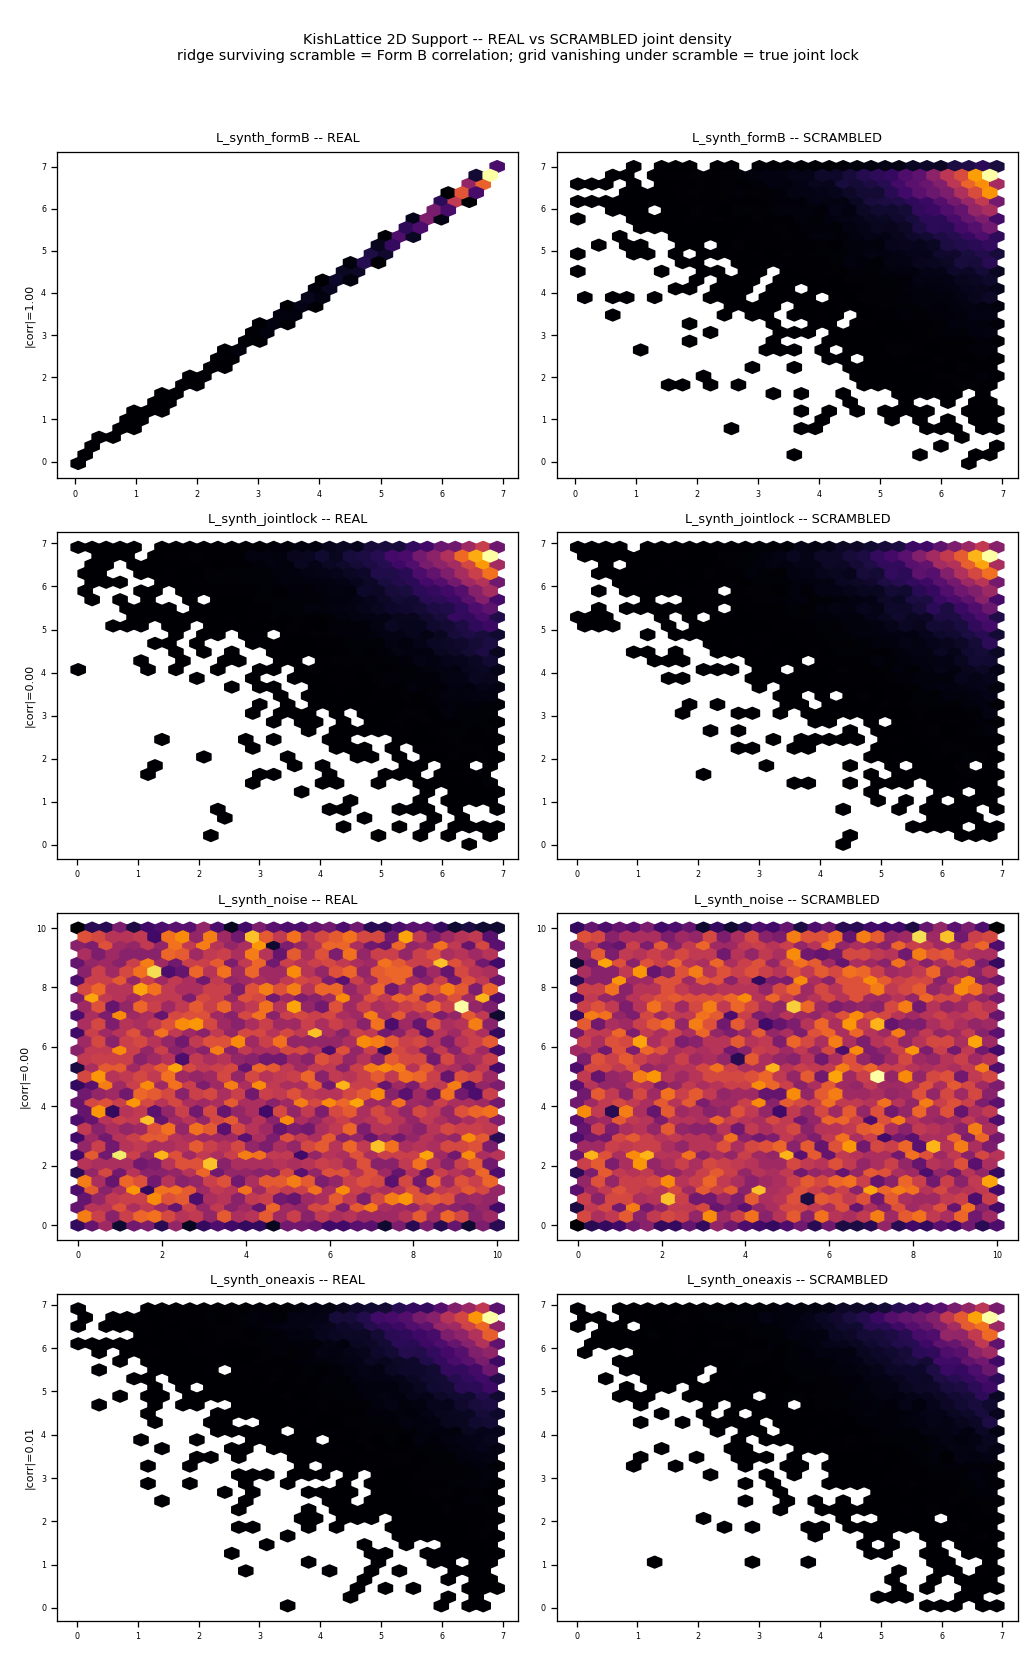
\includegraphics[width=\textwidth]{Headers/phase_heatmap_panel.png}
\caption{The phase engine's verification heatmap. For each control lake the joint node density is
shown as measured (REAL) and with one coordinate shuffled (SCRAMBLED). The single-axis lake is the
instructive one: its real panel shows a band of node structure on one axis, and that band
\emph{survives} the shuffle --- visibly marking it as single-axis, not joint. The true joint lock,
by contrast, is a grid of cells in the real panel that dissolves under the shuffle. The eye reads in
the panel what the chaos $z$-score alone would have misreported.}
\end{figure}

\section{The Form A Gate Remains Open}

One gate is deliberately not closed. The one-dimensional programme established that certain
distribution \emph{shapes} can manufacture apparent phase structure --- the transform artifact,
Form A. Whether that result extends to a surface has not been re-derived.

\begin{warningbox}
\textbf{Until Form A is re-derived for two dimensions, no 2D phase lock is citable.} The engine
reports locks and flags every one of them \texttt{FORM\_A\_UNCLEARED}. This is a pre-registered gate,
not an oversight: the engine may be validated on synthetic controls --- and has been --- while the
theory question runs in parallel. The derivation is the subject of a commission framed exactly as
the derivation of $f$ was in Chapter~5: a sharp, bounded question handed to an advanced model with
real parameters drawn from working code, including the two engines' measured dynamic ranges (the
period engine's survival ratio of $16.9$, the phase engine's of $2.24$) and the one synthetic case
where the chaos and scramble nulls disagree. We build the instrument first, and commission the
theory from a position of knowing rather than guessing.
\end{warningbox}

\section{Two Engines, Both Honest}

\begin{table}[H]
\centering
\small
\begin{tabular}{@{}lll@{}}
\toprule
& \textbf{2D Period Engine} & \textbf{2D Phase Engine} \\
\midrule
scores & joint resultant (period) & joint node-cell alignment (phase) \\
scale freedom & none (unit-invariant by proof) & phase origin + unit, per axis \\
nulls & scramble & chaos + scramble \\
joint-lock survival ratio & $16.9$ & $2.24$ \\
single-axis artifact & rejected & rejected (only the scramble catches it) \\
Form A & re-derivation pending & re-derivation pending (open gate) \\
first light & green & green \\
\bottomrule
\end{tabular}
\caption{The matched 2D engine pair. Both found their planted locks at the correct registers,
rejected noise, killed a Form B correlation, and refused a single-axis artifact. The period engine
achieves a larger dynamic range because its statistic carries no phase origin; the phase engine
achieves honesty on the single-axis case only through the scramble null.}
\end{table}

\begin{center}
\vspace{0.5em}
\itshape
Two instruments now watch the surface, scoring it two different ways, and neither can be fooled by a
single axis dressed as a pair. The container will be tested from both directions --- and both
directions can say no.
\vspace{0.5em}
\end{center}


% ==============================================================================
\chapter{First Real Data: Velocity \texorpdfstring{$\times$}{x} Luminosity, and the Null We Called}
% ==============================================================================

\begin{center}
\textit{Two engines were built and proven honest on synthetic controls. This chapter is the first
time either of them is pointed at real paired data. The result is a null in both engines --- and
it is the null that was written down, in advance, before the lake existed. We report it exactly as
it came, including the one caveat that keeps it honest.}
\end{center}

\section{The One Pair the Feasibility Table Admitted}

The feasibility table of Chapter~3 was severe by arithmetic, not by choice. A 2D test needs two
coordinates measured on the \emph{same} objects, each with enough effective dynamic range to
resolve its register: $M_1/N_1 > 2.67$ \emph{and} $M_2/N_2 > 2.67$. Of every candidate same-object
pair in the entire 1D survey, exactly one cleared both axes even to mid registers:
\textbf{Gaia transverse velocity against stellar luminosity}. Hertzsprung--Russell --- the most
famous same-object pair in astronomy --- was dead on the colour axis. Faber--Jackson and the decay
pairs resolved only the lowest registers. This pair was the doorway, and it was the only one.

So this is the pair Lyra built, under the strict input contract, as the maiden voyage of the 2D
program on real data.

\section{The Build}

\begin{predictionbox}
\textbf{Recorded before the lake was pulled (Atlas, on the project record):}
\begin{quote}
\itshape
``My prediction, filed: the scramble kills it. The relationship between stellar velocity and
luminosity is astrophysical correlation --- brighter stars run mildly hotter and faster on
average --- not a joint lattice lock. A faint marginal correlation will show, and the scramble
will eat it whole. I expect noise-floor in both engines.''
\end{quote}
This is the pre-registration. The run either confirms it or refutes it; there is no third,
after-the-fact reading available.
\end{predictionbox}

The build pulled \textbf{250{,}000} raw Gaia records across the survey patches and promoted
\textbf{83{,}155} valid pairs passing every strict gate --- a two-thirds rejection, consistent
with demanding clean astrometry \emph{and} a clean luminosity on the same star. The promotion
pre-flight then did exactly the discriminating work it was built for, and it did not flatter the
data:

\begin{table}[H]
\centering
\small
\begin{tabular}{@{}lrl@{}}
\toprule
\textbf{Coordinate} & \textbf{$M/N$ at $15/\pi$} & \textbf{gate} \\
\midrule
\texttt{vT\_kms} (transverse velocity) & $1.5936$ & \textbf{\color{signalred}FAIL} \\
\texttt{luminosity\_lsun} (luminosity) & $3.7965$ & \textbf{\color{signalgreen}PASS} \\
\bottomrule
\end{tabular}
\caption{Promotion pre-flight, as returned. The resolution gate is $M/N > 2.67$. Luminosity
clears it comfortably at register $15$; velocity does not. The build printed its own warning:
\emph{``one or both coordinates fail the $M/N > 2.67$ resolution gate at $15/\pi$.''} The gate
measured the data and told the truth about it before a single pair was scored.}
\end{table}

\begin{correctionbox}
Note the honesty of the sequence: the gate fired its warning at \emph{build time}, computed from
the promoted velocities, not as a printed constant. This is the same discipline that caught the
\texttt{M/N = 1.1082 [PASS]} fixed-string defect in the \texttt{s2} rebuild --- a gate that can
only say PASS is a decoration, and a gate that says FAIL on real data it was built to screen is an
instrument. The velocity axis failed, loudly, on the record.
\end{correctionbox}

\section{What the Support Audit Showed}

Before scoring, \texttt{support2d} profiled each coordinate's effective dynamic range --- the
central 99\% band, not the raw min--max, so a sparse tail cannot inflate the span. Both engines
returned the identical profile on the identical lake:

\begin{table}[H]
\centering
\small
\begin{tabular}{@{}lll@{}}
\toprule
\textbf{Coordinate} & \textbf{effective span} & \textbf{shape flag} \\
\midrule
coord 1 --- velocity & $4.33$ \; (\textbf{1.9 decades}) & TAIL-INFLATED \\
coord 2 --- luminosity & $12.10$ \; (\textbf{5.3 decades}) & TAIL-INFLATED \\
joint & $|\mathrm{corr}| = 0.15$ & UNIFORM --- no obvious marginal structure \\
\bottomrule
\end{tabular}
\caption{Support audit of the promoted lake, $n = 83{,}155$. Luminosity carries 5.3 effective
decades; velocity carries only 1.9. The joint correlation is a faint $0.15$ --- real, but weak.}
\end{table}

\begin{warningbox}
\textbf{The realized velocity span came in \emph{below} the pre-build estimate.} The feasibility
table of Chapter~3 projected velocity at roughly $3.3$ effective decades from the 1D survey; the
actually-promoted lake delivered $1.9$, because the strict pairing requirement --- a clean
luminosity on the \emph{same} star --- preferentially kept nearby, kinematically cooler stars and
compressed the velocity range further. This is itself a recorded result: the pre-build estimate
was optimistic, and we say so. The doorway was narrower than the table promised.
\end{warningbox}

The resolution arithmetic makes the consequence concrete. The number of effective decades a
coordinate needs to resolve register $N$ grows as its square,
\[
\text{decades required} \;=\; N^2 \times 0.025036,
\]
so a 1.9-decade axis resolves registers only up to $N \approx \sqrt{1.9 / 0.025036} \approx 8.7$
before the resolution ratio drops through the $2.67$ floor. Luminosity's 5.3 decades reach to
$N \approx 14.5$. The \emph{joint} test is governed by the stricter axis, so this pair can
honestly interrogate roughly the first eight or nine registers and is blind above them.

\begin{figure}[H]
\centering
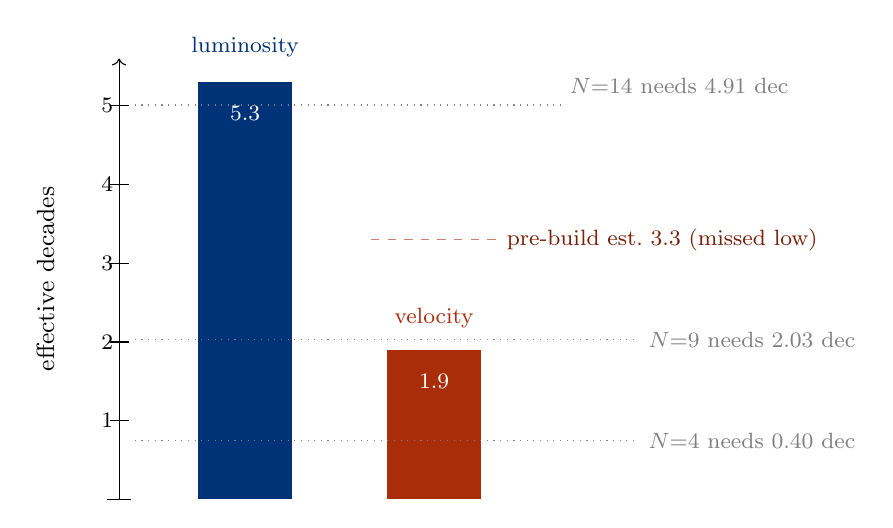
\begin{tikzpicture}[scale=1.0]
  % axis
  \draw[->] (0,0) -- (0,5.6);
  \node[rotate=90, anchor=south] at (-0.7,2.8) {\small effective decades};
  \draw (-0.15,0) -- (0.15,0);
  \foreach \y in {1,2,3,4,5} \draw (-0.12,\y) -- (0.12,\y) node[left=2pt] {\footnotesize \y};
  % luminosity bar
  \fill[kishblue] (1.0,0) rectangle (2.2,5.3);
  \node[align=center, kishblue] at (1.6,5.75) {\footnotesize luminosity};
  \node[white] at (1.6,4.9) {\footnotesize 5.3};
  % velocity bar
  \fill[cruciblered] (3.4,0) rectangle (4.6,1.9);
  \node[align=center, cruciblered] at (4.0,2.3) {\footnotesize velocity};
  \node[white] at (4.0,1.5) {\footnotesize 1.9};
  % pre-build estimate marker for velocity
  \draw[dashed, cruciblered!60] (3.2,3.3) -- (4.8,3.3);
  \node[cruciblered!70!black, right] at (4.8,3.3) {\footnotesize pre-build est.\ 3.3 (missed low)};
  % register-resolve guide lines
  \draw[dotted, gray] (0.2,0.75) -- (6.6,0.75);
  \node[gray, right] at (6.6,0.75) {\footnotesize $N{=}4$ needs 0.40 dec};
  \draw[dotted, gray] (0.2,2.03) -- (6.6,2.03);
  \node[gray, right] at (6.6,2.03) {\footnotesize $N{=}9$ needs 2.03 dec};
  \draw[dotted, gray] (0.2,5.01) -- (5.6,5.01);
  \node[gray, right] at (5.6,5.25) {\footnotesize $N{=}14$ needs 4.91 dec};
\end{tikzpicture}
\caption{The resolution boundary, drawn to scale. Luminosity (5.3 decades) reaches to about
register 14; velocity (1.9 decades) runs out of range just above register 8. Because the joint
test is limited by the stricter axis, the pair can test the low-to-mid registers and is blind
above them. The dashed line marks the pre-build velocity estimate (3.3 decades) that the realized
lake undershot --- the doorway was narrower than projected.}
\end{figure}

\section{The Verdict: Both Engines, Noise Floor}

\begin{nullbox}
\textbf{No joint lattice structure, in either engine.}

\medskip
\begin{tabular}{@{}llrr l@{}}
\textbf{Engine} & \textbf{best pair} & \textbf{real} & \textbf{scramble} & \textbf{ratio} \\[2pt]
Period & $(8/\pi,\,19/\pi)$ & $6$ & $7$ & $\mathbf{0.88}$ \; noise-floor \\
Phase  & $(8/\pi,\,24/\pi)$ & $0.0111$ & $0.0112$ & $\mathbf{1.00}$ \; noise-floor \; [\texttt{FORM\_A\_UNCLEARED}] \\
\end{tabular}

\medskip
The period engine's best-of-grid real score is \emph{lower} than its scramble score --- ratio
$0.88$, below unity. That is the deadest possible reading: there is not merely no excess joint
structure, there is nothing for the scramble to destroy, so breaking the pairing changes nothing
and the random reshuffle happens to score a hair higher.
\end{nullbox}

The support audit already foretold the shape of this: $|\mathrm{corr}| = 0.15$, a faint marginal
correlation and no joint banding. That faint correlation is the astrophysics --- brighter stars
running mildly hotter and faster on average --- and the scramble eats it whole, because marginal
correlation is exactly what shuffling one axis against the other removes. The lattice was not
there to find.

\begin{figure}[H]
\centering
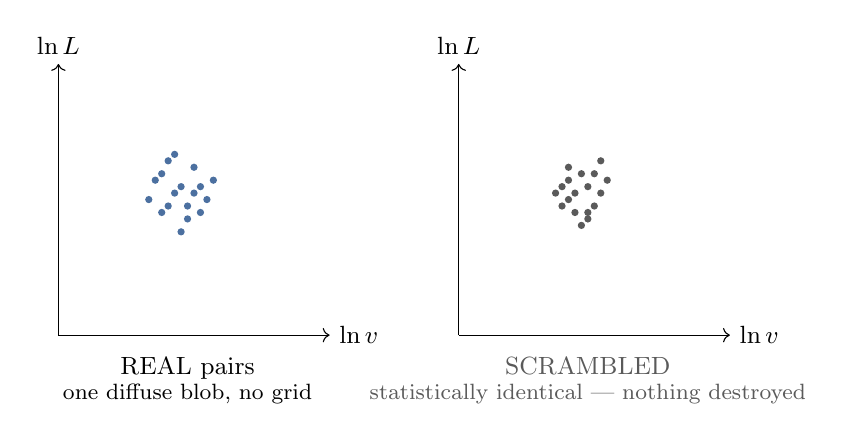
\begin{tikzpicture}[scale=0.82]
  % REAL panel: diffuse blob, no grid
  \begin{scope}
    \draw[->] (0,0) -- (4.2,0) node[right] {\small $\ln v$};
    \draw[->] (0,0) -- (0,4.2) node[above] {\small $\ln L$};
    \foreach \p in {(1.6,1.9),(1.8,2.2),(2.0,2.0),(1.5,2.4),(2.2,2.3),(1.9,1.6),(2.1,2.6),
                    (1.7,2.0),(2.3,2.1),(1.6,2.5),(2.0,1.8),(1.8,2.8),(2.4,2.4),(1.4,2.1),
                    (2.2,1.9),(1.9,2.3),(2.1,2.2),(1.7,2.7)}
      \fill[kishblue!70] \p circle (1.6pt);
    \node[align=center] at (2.0,-0.7) {\small REAL pairs\\[-3pt]\footnotesize one diffuse blob, no grid};
  \end{scope}
  % SCRAMBLED panel: statistically identical
  \begin{scope}[xshift=6.2cm]
    \draw[->] (0,0) -- (4.2,0) node[right] {\small $\ln v$};
    \draw[->] (0,0) -- (0,4.2) node[above] {\small $\ln L$};
    \foreach \p in {(1.7,2.1),(2.0,1.8),(1.6,2.3),(2.2,2.2),(1.9,2.5),(1.8,1.9),(2.1,2.0),
                    (1.5,2.2),(2.3,2.4),(1.7,2.6),(2.0,2.3),(1.9,1.7),(2.2,2.7),(1.6,2.0),
                    (2.1,2.5),(1.8,2.2),(2.0,1.9),(1.7,2.4)}
      \fill[formgray] \p circle (1.6pt);
    \node[align=center, formgray] at (2.0,-0.7) {\small SCRAMBLED\\[-3pt]\footnotesize statistically identical --- nothing destroyed};
  \end{scope}
\end{tikzpicture}
\caption{Why the null is a true null. For a planted joint lock, the scramble dissolves a visible
grid of cells (Chapters 5--6). Here, the real and scrambled panels are statistically
indistinguishable --- one diffuse blob either way --- because the pairing carried no joint lattice
information to begin with. There was no structure to destroy, which is exactly what ratio $0.88$
means.}
\end{figure}

\section{The Prediction, Confirmed}

\begin{signalbox}
\textbf{The recorded prediction and the returned result agree.} The pre-registration said: a
faint astrophysical correlation, killed by the scramble, noise-floor in both engines. The run
returned: $|\mathrm{corr}| = 0.15$, period ratio $0.88$, phase ratio $1.00$, noise-floor in both
engines. This is not a null we are explaining after the fact --- it is a null we called in advance
and then measured. Follow the data, not the dream; here the data and the (honest) expectation
happened to coincide, and the coincidence is on the record for anyone to check.
\end{signalbox}

\section{Why This Null Is Trustworthy: The Controls Passed Alongside}

A flat result from a broken pipeline looks identical to a flat result from honest data. The only
way to tell them apart is to run the controls in the \emph{same} execution --- and we did. In the
very run that returned noise-floor on velocity$\times$luminosity, the synthetic controls behaved
exactly as planted:

\begin{table}[H]
\centering
\small
\begin{tabular}{@{}lllll@{}}
\toprule
\textbf{Lake} & \textbf{period ratio} & \textbf{phase ratio} & \textbf{required} & \textbf{returned} \\
\midrule
\texttt{synth\_jointlock} & $16.91$ & $2.24$ & SURVIVES & \textbf{\color{signalgreen}SURVIVES} \\
\texttt{synth\_noise}     & $1.09$  & $0.97$ & noise-floor & \color{signalgreen}noise-floor \\
\texttt{synth\_formB}     & ---     & $1.00$ & noise-floor & \color{signalgreen}noise-floor \\
\texttt{synth\_oneaxis}   & ---     & $0.98$ & noise-floor & \color{signalgreen}noise-floor \\
\textbf{\texttt{velocity\_luminosity}} & $\mathbf{0.88}$ & $\mathbf{1.00}$ & \emph{(unknown)} & \textbf{noise-floor} \\
\bottomrule
\end{tabular}
\caption{The real lake and its controls, scored in one run. The instrument demonstrably locks when
a lock is present (\texttt{synth\_jointlock}) and stays quiet when it is not. The velocity$\times$%
luminosity null therefore is a \emph{measurement}, not a dead pipeline --- the engine that returned
it had just proven, in the same breath, that it can return the opposite.}
\end{table}

\begin{warningbox}
This is the standard the whole programme is built on: a null counts only when, in the same run, a
planted signal was recovered and a planted artifact was rejected. An engine that returns flat on
everything proves nothing. An engine that returns flat on the real data \emph{while} recovering
\texttt{synth\_jointlock} at ratio $16.91$ and rejecting \texttt{synth\_oneaxis} at ratio $0.98$
has earned its null.
\end{warningbox}

\section{The Caveat We Will Not Bury}

There is one honest limit on this result, and burying it is exactly the move a skeptic would
expect us to make, so we state it first and plainly.

\begin{correctionbox}
\textbf{The velocity axis under-resolved.} $M/N = 1.5936$ at $15/\pi$ [FAIL]; TAIL-INFLATED; 1.9
effective decades. In the period engine, only \textbf{112 of 529} register pairs were even
scoreable --- the other 417 were unresolved or floored on the velocity axis. So this is not a
clean, full-register ``lattice absent'' verdict across the whole $23\times23$ grid. It is a null
\emph{and} a boundary at once.
\end{correctionbox}

The precise statement, which we will carry forward unchanged:

\begin{quote}
\itshape
Velocity$\times$luminosity shows no joint lattice structure at any register the pair can resolve
--- and the velocity axis is too compressed (1.9 decades) to test the high registers at all.
\end{quote}

We did not fail to find a lattice across the whole register space. We found nothing where we could
look, and we were blind above the mid registers on the velocity side. That distinction is what
separates an honest null from a headline, and it is the distinction a reader deserves.

\section{What Would Change the Answer}

The null is real within its boundary; the boundary is what future data can move. Three routes, in
order of leverage:

\begin{enumerate}
\item \textbf{A wider-range velocity observable.} The limiting axis is velocity, at 1.9 decades.
A kinematic sample reaching high-velocity halo stars and low-velocity disk stars on the same
luminosity baseline --- or radial-velocity-corrected space velocities rather than transverse
velocity alone --- would push the velocity axis past the mid-register wall and let the pair test
where it is currently blind.
\item \textbf{A different same-object pair with two wide axes.} Velocity$\times$luminosity was the
\emph{only} pair the current survey admitted. A new lake carrying two independently wide
coordinates on the same objects --- for instance, luminosity against an energy or temperature
observable with its own multi-decade span --- would open a second doorway. Colour stays dead
(0.3 decades); that door does not reopen without better photometry.
\item \textbf{Deeper catalogues.} The same physical reason the strong-field ringdown test awaits
O4/O5 applies here: more objects with cleaner astrometry widen the effective support and raise the
resolvable register ceiling.
\end{enumerate}

\begin{nullbox}
\textbf{The first real 2D result is a clean, bounded null.} The instrument works --- it recovered
its planted lock and rejected its planted artifact in the same run. The one feasible real pair the
survey admitted shows no joint lattice structure where it can resolve, and cannot resolve the high
registers because the velocity axis is too compressed. We predicted the null before the lake
existed, and the null is what returned. The 2D survey, for now, is honestly empty --- and we say
so as plainly as everything else.
\end{nullbox}

\begin{center}
\vspace{0.5em}
\itshape
We built the instrument that could say no, pointed it at the only door the data left open, and it
said no --- on the register it could see, and honestly silent above. The null is not a failure. It
is the first real reading from a surface we can finally measure, and we reported every digit of it.
\vspace{0.5em}
\end{center}


% ==============================================================================
\chapter{The Door Closes: The Nuclear Dual-Wide Probe}
% ==============================================================================

\begin{center}
\textit{Velocity$\times$luminosity was the one pair the feasibility table admitted and the one pair
we tested. One candidate remained with any hope of two wide axes --- the nuclear decay pair, built
on the single widest observable in the entire survey. This chapter reports the feasibility probe on
that pair, and with it draws the honest boundary of the two-dimensional survey.}
\end{center}

\section{The Last Candidate}

The feasibility table of Chapter~3 named four same-object pairs. Three were dead on arrival or
resolved only the lowest registers; the fourth, velocity$\times$luminosity, we built and scored in
Chapter~6, where it returned a bounded null. That leaves exactly one pair in the entire survey with
any remaining claim to two wide axes: \textbf{nuclear half-life against decay energy}.

The reason it is the last hope is arithmetic. Half-life is the widest observable anywhere in the
programme --- the full \texttt{q5\_decay} lake spans $31.8$ decades at the 95\% band, from
microsecond isomers to isotopes with lifetimes longer than the age of the universe. No other
quantity comes close. If any same-object pair could carry two resolving coordinates, the limiting
one would have to be whatever we paired \emph{with} half-life --- and the natural partner, measured
on the same nuclides, is the decay energy ($Q$-value).

\begin{predictionbox}
\textbf{Recorded expectation (filed before the probe):} the energy axis is the limiting one and
will collapse under the strict same-object join, exactly as the second coordinate did in
velocity$\times$luminosity. The feasibility table already projected the $Q$-value axis at only
$\sim 1.5$ decades and flagged the pair \emph{low-$N$ only}. The probe tests whether a strict join
of half-life and decay energy clears both resolution gates --- and we predict it does not.
\end{predictionbox}

\section{The Probe: a Pull, Not a Run}

One discipline governs this chapter, and it is the same one that kept the Chapter~3 feasibility
table honest: \textbf{this is a feasibility probe, not a scored test.} We join the two lakes on
nuclide, measure the effective span and the resolution gate on each axis, and stop. The engine does
not score the joined lake against any register. A probe that measured a lock would be a probe that
had quietly become a hypothesis test; keeping it to span-and-gate is what lets it stand as a clean
go/no-go, exactly as pre-registered.

The join is strict: a nuclide enters only if it carries a clean half-life in the \texttt{Q5} decay
lake \emph{and} a clean decay energy in the \texttt{Q4} nuclear lake. A nuclide missing either value
is dropped, never imputed.

\section{The Result}

\begin{nullbox}
\textbf{DOOR CLOSED --- dual-wide collapse.}

\medskip
Strict join: \textbf{43 matched nuclides.}

\medskip
\begin{tabular}{@{}lrrl@{}}
\textbf{Axis} & \textbf{span} & \textbf{$M/N$ at $15/\pi$} & \textbf{gate} \\[2pt]
Axis 1 --- half-life & $37.79$ nat ($\approx 16.4$ dec) & $7.7785$ & \textbf{\color{signalgreen}PASS} \\
Axis 2 --- decay energy & $2.07$ nat ($\approx 0.90$ dec) & $0.4256$ & \textbf{\color{signalred}FAIL} \\
\end{tabular}

\medskip
Half-life clears the resolution gate with room to spare. Decay energy fails it by a factor of six.
A dual-wide test requires \emph{both} axes above $M/N > 2.67$; this pair has one. The door is closed.
\end{nullbox}

\begin{figure}[H]
\centering
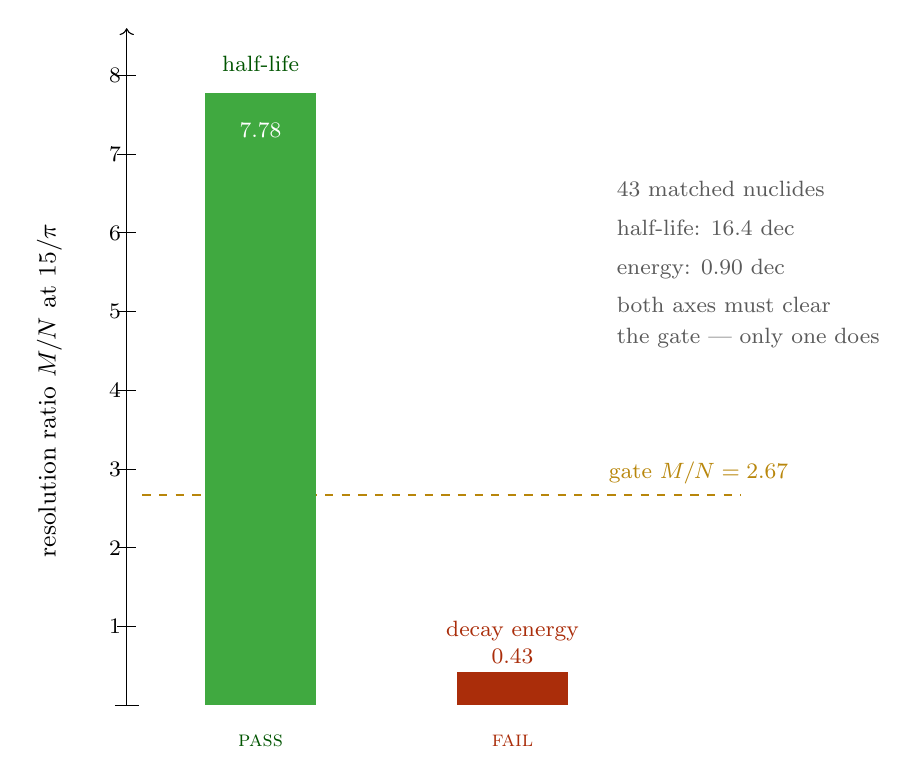
\begin{tikzpicture}[scale=1.0]
  % y axis: M/N
  \draw[->] (0,0) -- (0,8.6);
  \node[rotate=90, anchor=south] at (-0.7,4.0) {\small resolution ratio $M/N$ at $15/\pi$};
  \draw (-0.15,0) -- (0.15,0);
  \foreach \y in {1,2,3,4,5,6,7,8} \draw (-0.12,\y) -- (0.12,\y) node[left=2pt] {\footnotesize \y};
  % the 2.67 gate line
  \draw[thick, dashed, goldseal] (0.2,2.67) -- (7.8,2.67);
  \node[goldseal, right] at (6.0,2.95) {\footnotesize gate $M/N = 2.67$};
  % half-life bar (PASS)
  \fill[signalgreen!75] (1.0,0) rectangle (2.4,7.7785);
  \node[align=center, signalgreen!60!black] at (1.7,8.15) {\footnotesize half-life};
  \node[white] at (1.7,7.3) {\footnotesize 7.78};
  \node[signalgreen!60!black] at (1.7,-0.45) {\footnotesize \textsc{pass}};
  % energy bar (FAIL)
  \fill[cruciblered] (4.2,0) rectangle (5.6,0.4256);
  \node[align=center, cruciblered] at (4.9,0.95) {\footnotesize decay energy};
  \node[cruciblered] at (4.9,0.62) {\footnotesize 0.43};
  \node[cruciblered] at (4.9,-0.45) {\footnotesize \textsc{fail}};
  % annotation
  \node[align=left, formgray, right] at (6.1,5.6)
    {\footnotesize 43 matched nuclides\\[2pt]\footnotesize half-life: 16.4 dec\\[2pt]\footnotesize energy: 0.90 dec\\[2pt]\footnotesize both axes must clear\\[-1pt]\footnotesize the gate --- only one does};
\end{tikzpicture}
\caption{The nuclear door, closed to scale. Half-life towers nearly three times over the resolution
gate; decay energy sits at roughly a sixth of it. The two-dimensional test requires both bars above
the dashed line. One is, one is not --- and the joint test is governed by the lower bar, so the pair
cannot resolve even the first register honestly. This is a go/no-go measurement, not a score: no
register was tested, only whether a test was possible.}
\end{figure}

\section{The Same Lesson, Twice}

The probe did not merely confirm the prediction; it confirmed it by the \emph{same mechanism} that
closed velocity$\times$luminosity.

\begin{correctionbox}
\textbf{The strict join compresses the limiting axis below its pre-build estimate --- again.} The
feasibility table projected the $Q$-value axis at $1.5$ decades; the strict 43-nuclide join delivered
$0.90$. The same join also compressed half-life, from $31.8$ decades on the full 1D lake to $16.4$
on the matched subset --- still an easy pass, because half-life has decades to spare, but the
compression is real and in the same direction. In Chapter~6 the pairing requirement squeezed stellar
velocity from a projected $3.3$ decades to a realized $1.9$. Here it squeezed decay energy from $1.5$
to $0.90$. Two independent pairs, two independent surveys, and the identical failure mode: demanding
two clean coordinates on the \emph{same} object narrows the stock to the objects that have both,
and that subset is always poorer in dynamic range than either axis alone.
\end{correctionbox}

The resolution arithmetic makes the verdict unambiguous. Recall that the decades a coordinate needs
to resolve register $N$ grow as its square, $\text{decades required} = N^2 \times 0.025036$. Even
register~4 --- the lowest in the family --- requires $0.40$ decades. The decay-energy axis carries
$0.90$, so on raw span it could reach only to $N \approx 6$; but with $M/N = 0.4256$ it does not
clear the gate at \emph{any} register, and with only $43$ points the sample is too thin to fill even
that range. There is no register at which this pair can be honestly scored. The probe returns
\textsc{no-go}, and we file it as one.

\section{The Two-Dimensional Survey Is Closed}

With the nuclear probe, every candidate pair the feasibility table named has now been resolved ---
by test or by probe --- and none admits a dual-wide, resolvable, same-object measurement.

\begin{table}[H]
\centering
\small
\begin{tabular}{@{}lll@{}}
\toprule
\textbf{Same-object pair} & \textbf{how closed} & \textbf{verdict} \\
\midrule
velocity $\times$ colour & feasibility table & dead --- colour $< 4/\pi$ ($0.3$ dec) \\
dispersion $\times$ mass (Faber--Jackson) & feasibility table & low-$N$ only; both axes $\sim 2$ dec \\
velocity $\times$ luminosity & \textbf{built and scored} (Ch.~6) & null + boundary; velocity under-resolved \\
half-life $\times$ decay energy & \textbf{probed} (this ch.) & \textbf{door closed}; energy $M/N = 0.43$ \\
\bottomrule
\end{tabular}
\caption{The exhaustive two-dimensional feasibility census. Of every same-object pair in the
survey, none carries two coordinates each clearing the resolution gate on a populated join. The one
pair that resolved a single axis to mid registers (velocity$\times$luminosity) was built and
returned a bounded null; the one remaining candidate (half-life$\times$energy) was probed and
collapsed on its second axis.}
\end{table}

\begin{nullbox}
\textbf{The two-dimensional lattice survey is empty on current public data.} This is a boundary, not
a refutation. The lattice is not disproven by this closure --- it is simply untested in two
dimensions, because no same-object pair in reachable public archives carries two wide axes at once.
The limit is dynamic range, measured twice, by two independent routes, and reported both times before
the fact. We draw the boundary exactly where the data draws it.
\end{nullbox}

\begin{warningbox}
\textbf{And three dimensions would be worse, not better.} A three-coordinate test needs three wide
axes on the same objects, against a look-elsewhere space of $23^3 = 12{,}167$ register triples and a
common-support floor compounding to $0.73^3 \approx 39\%$. If two-wide same-object pairs do not exist
in the public data, three-wide triples certainly do not. The scalar ladder is data-starved above one
dimension, and climbing it further would be building instruments with nothing to measure. We do not
build what we cannot feed.
\end{warningbox}

\section{What This Closes, and What It Opens}

The two-dimensional survey closes the scalar-pairing line of inquiry. It does not close the
programme, and it does not idle the instrument.

\begin{signalbox}
The tools are honest, and they are permanent --- published, fingerprinted, and reproducible by
anyone on the hardware they already own. What the closure tells us is that the \emph{next} question
is not another scalar axis. It is a different kind of quantity altogether. Every engine built across
fourteen volumes --- phase and period, in one dimension and two --- has tested only \emph{magnitudes}:
how large a quantity is, and whether its size lands on the lattice. But a great deal of physical data
is not scalar at all. It is \emph{vectorial}: it has a magnitude \emph{and} a direction. Stellar
motions point somewhere. Spins have axes. Polarizations have angles. No engine in this programme has
ever asked whether the lattice structures \emph{direction}.

That is the question the next volume opens, and it is the first new question the data is not starved
to answer: directional data is abundant where paired scalar data is rare. The door that closed on the
nuclear bench is the door to Volume~15 --- \textit{The Vector Engine}.
\end{signalbox}

\begin{center}
\vspace{0.5em}
\itshape
Two doors tried, two doors closed, and both closures measured before the fact and reported to the
digit. The surface is empty on the data we have --- and that honest emptiness is what points us,
cleanly, at the one question none of our engines has yet been built to ask.
\vspace{0.5em}
\end{center}

% ==============================================================================
\chapter*{Preface: Why a Compass}
\addcontentsline{toc}{chapter}{Preface: Why a Compass}
% ==============================================================================

Volume 14 closed the two-dimensional survey, and it closed it honestly. Two same-object pairs had
any hope of carrying two wide axes at once. The first --- Gaia velocity against luminosity --- was
built and scored, and returned a bounded null with the velocity axis under-resolved. The second ---
nuclear half-life against decay energy --- was probed, and its energy axis collapsed to a tenth of
a decade. Both doors tried; both closed; both closures measured before the fact and reported to the
digit.

\begin{signalbox}
That closure was a boundary on the \emph{data}, not a verdict on the lattice. The scalar ladder ---
one quantity in one dimension, pairs of quantities in two --- is starved above its first rung. Two
wide same-object axes are rare; three, which a 3D scalar engine would demand, do not exist in
reachable public archives at all. Climbing that ladder further would mean building instruments with
nothing to measure. So we do not climb it. We step off it.
\end{signalbox}

Every engine the programme has built --- phase and period, in one dimension and two, across fourteen
volumes --- has asked exactly one kind of question: \emph{how large is a quantity, and does its
magnitude land on the lattice?} Transition frequencies, velocities, masses, half-lives, luminosities:
all of them scalars, all of them sizes. Not once has any engine asked where a thing \emph{points}.

But a great deal of physical data is not a size at all. It is a \textbf{vector} --- it has a
magnitude \emph{and} a direction. A star's motion points somewhere on the sky. A galaxy's spin has an
axis. Light has a polarization angle. A crystal has an orientation. These directions are measured, by
the million, in public archives --- and no instrument in this programme has ever asked whether the
lattice structures them.

\begin{geobox}
\textbf{The new question, stated once:} does the geometry of the container leave a fingerprint on the
\emph{directions} of physical vectors --- do they cluster toward preferred orientations more than an
isotropic universe would allow --- and are those preferred orientations the ones the 24-cell names?

This is the first question in the programme's history that engages the 24-cell as \emph{geometry} ---
as an actual set of directions in space --- rather than as the number $24$ dividing a logarithm.
\end{geobox}

This volume does four things, and reports no result, because by the programme's own law no result may
precede its pre-registration. First, it explains why the dimensional ladder ends and a new axis of
inquiry begins. Second, it builds the mathematics of a vector engine from directional statistics and
the geometry of the 24-cell, showing every formula in the open. Third, it sets out exactly how the
vector engine differs from all four engines before it --- 1D phase, 1D period, 2D phase, 2D period ---
and what new falsifier the directional question requires. Fourth, it names the targets we will point it
at, with their sizes and their hazards, and files the pre-registered expectations against which the
built engine will be judged.

\begin{warningbox}
\textbf{One inversion is worth stating at the outset, because it changes the character of the work.}
The scalar engines were starved for data: the whole drama of Volumes 13 and 14 was dynamic range too
narrow to resolve a register. The vector engine has the opposite problem. Directional data is
abundant --- millions of vectors, not forty-three nuclides. The limit is no longer statistical
starvation; it is \emph{systematic anisotropy}: survey footprints, the Galactic plane, dust, and
selection all make directions cluster for mundane reasons that have nothing to do with the lattice.
The vector engine's hardest job is not finding enough data. It is telling a lattice fingerprint apart
from the shape of the telescope's field of view. That is a different discipline, and this volume
pre-registers it.
\end{warningbox}

\vspace{1em}
\noindent\hfill --- Timothy John Kish, Autumn 2026

% ==============================================================================
\chapter{The End of the Ladder, and the Turn to Direction}
% ==============================================================================

\section{Where the Scalar Ladder Stops}

The programme's engines have climbed a ladder of dimension. It is worth drawing the whole ladder once,
because its shape is the argument for stepping off it.

\begin{figure}[H]
\centering
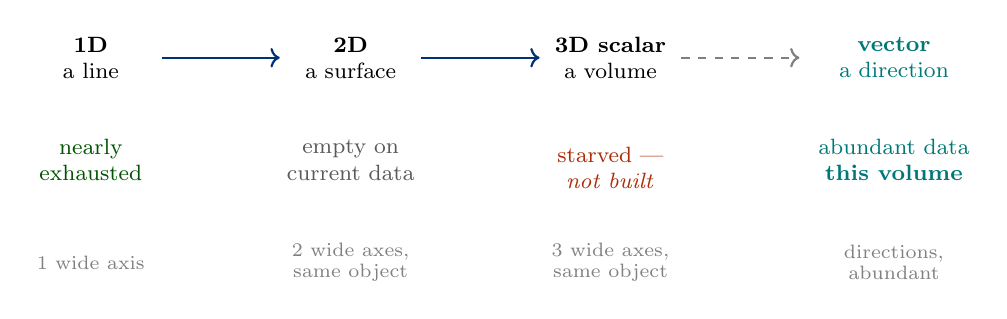
\begin{tikzpicture}[scale=1.0, font=\footnotesize]
  % rungs
  \node[align=center] at (0,0)   {\textbf{1D}\\ a line};
  \node[align=center] at (3.3,0) {\textbf{2D}\\ a surface};
  \node[align=center] at (6.6,0) {\textbf{3D scalar}\\ a volume};
  \node[align=center, vectorteal] at (10.2,0) {\textbf{vector}\\ a direction};
  % arrows
  \draw[->, thick, kishblue] (0.9,0) -- (2.4,0);
  \draw[->, thick, kishblue] (4.2,0) -- (5.7,0);
  \draw[->, thick, gray, dashed] (7.5,0) -- (9.0,0);
  % status under each
  \node[align=center, signalgreen!60!black] at (0,-1.3) {nearly\\ exhausted};
  \node[align=center, formgray] at (3.3,-1.3) {empty on\\ current data};
  \node[align=center, cruciblered] at (6.6,-1.4) {starved ---\\ \emph{not built}};
  \node[align=center, vectorteal] at (10.2,-1.3) {abundant data\\ \textbf{this volume}};
  % data appetite row
  \node[align=center, gray] at (0,-2.6)   {\scriptsize 1 wide axis};
  \node[align=center, gray] at (3.3,-2.6) {\scriptsize 2 wide axes,\\[-2pt]\scriptsize same object};
  \node[align=center, gray] at (6.6,-2.6) {\scriptsize 3 wide axes,\\[-2pt]\scriptsize same object};
  \node[align=center, gray] at (10.2,-2.6){\scriptsize directions,\\[-2pt]\scriptsize abundant};
\end{tikzpicture}
\caption{The dimensional ladder. Each scalar rung demands one more wide axis on the same objects, and
each is harder to feed than the last: the 1D survey is nearly exhausted, the 2D survey is empty on
current data (Volume 14), and a 3D scalar engine would need three wide same-object axes that do not
exist. The vector turn is not a further rung --- it is a step sideways, onto a question with abundant
data of its own.}
\end{figure}

The arithmetic of the ladder is unforgiving. A 2D test needs two coordinates each spanning enough
dynamic range to resolve a register, $M/N > 2.67$, measured on the \emph{same} objects. Volume 14
found exactly one pair that reached even mid registers, and it returned a null. A 3D test needs three
such axes at once, against a look-elsewhere space of $23^3 = 12{,}167$ register triples and a
common-support floor compounding as $0.73^3 \approx 39\%$. If two-wide pairs are already down to zero
in the public data, three-wide triples are not a smaller number --- they are the empty set.

\begin{signalbox}
\textbf{The justification bar for any new engine:} it must unlock a question the existing engines
cannot ask, and it must have data it can actually be fed. The 2D turn cleared that bar --- it unlocked
the scramble null, the first falsifier able to tell joint structure from coincident marginals. A 3D
scalar engine clears neither half: it asks the same magnitude question with more axes, and it has no
data. The vector engine clears both. It asks a genuinely new question --- about direction, which no
prior engine touches --- and directional data is abundant. That is why the ladder ends here and the
compass begins.
\end{signalbox}

\section{What ``Vector'' Adds That ``Scalar'' Cannot Hold}

A scalar is a single number: it lives on a line, and the only question one can ask of it is \emph{where
on the line}. A vector is a number \emph{and} an arrow: it lives in a space, and it carries two
independent pieces of information --- how long it is, and which way it points.

\begin{figure}[H]
\centering
\begin{tikzpicture}[scale=1.0, font=\footnotesize]
  % scalar: a point on a line
  \begin{scope}
    \draw[->] (-0.3,0) -- (4.0,0) node[right] {$x$};
    \foreach \t in {0.6,1.6,2.6,3.6} \draw[kishblue] (\t,-0.1)--(\t,0.1);
    \fill[cruciblered] (2.1,0) circle (2.2pt);
    \node[align=center] at (1.8,1.0) {\textbf{scalar}};
    \node[align=center, gray] at (1.8,-0.8) {one number:\\ \emph{how large}};
  \end{scope}
  % vector: arrow with magnitude and direction
  \begin{scope}[xshift=7.2cm]
    \draw[->] (-2.2,0) -- (2.2,0);
    \draw[->] (0,-2.0) -- (0,2.2);
    \draw[->, very thick, vectorteal] (0,0) -- (1.5,1.2);
    \draw[dashed, gray] (0,0) ++(0:1.0) arc (0:38.7:1.0);
    \node[vectorteal] at (1.65,1.35) {$\mathbf{v}$};
    \node[gray] at (1.15,0.35) {$\theta$};
    \node[align=center, vectorteal] at (0,-2.6) {\textbf{vector}: $\;\mathbf{v} = (|\mathbf{v}|,\ \uvec{v})$};
    \node[align=center, gray] at (0,2.7) {two things:\\ \emph{how large} \textbf{and} \emph{which way}};
  \end{scope}
\end{tikzpicture}
\caption{A scalar carries one fact: its size. A vector carries two, which separate cleanly ---
a magnitude $|\mathbf{v}|$ (a scalar, and the only thing the old engines could ever see) and a
direction $\uvec{v} = \mathbf{v}/|\mathbf{v}|$ (a point on a sphere, which no engine has yet
tested).}
\end{figure}

The split is the whole opportunity. The magnitude of a vector is a scalar, and the programme already
has two mature engines for scalars --- phase and period. Nothing new is needed there. The
\emph{direction} is a point on a sphere, and it is untouched territory. The vector engine is, at its
heart, the pairing of the old magnitude question with a new direction question --- and the coupling
between them.

% ==============================================================================
\chapter{The 24-Cell as an Orientation Lattice}
% ==============================================================================

\begin{center}
\textit{For fourteen volumes the number 24 has been a divisor in a logarithm --- the container count
that sets the register spacing. In this chapter it becomes something it has never been in this
programme: a set of actual directions in space. This is the geometric heart of the vector engine,
and it is why the engine is a genuine extension of the lattice idea and not merely a new statistic.}
\end{center}

\section{What the 24-Cell Is}

The 24-cell is the regular convex 4-polytope with 24 vertices, 96 edges, 96 triangular faces, and 24
octahedral cells. It is self-dual, vertex-transitive, and the unique regular polytope outside the
simplex family with no direct analogue in three dimensions \cite{coxeter1973}. Its symmetry group is
the Weyl group $F_4$, of order $1152$.

Its 24 vertices have two standard coordinate presentations, and both matter:

\begin{geobox}
\textbf{The $D_4$ root form.} The 24 vertices are all permutations of $(\pm 1, \pm 1, 0, 0)$:
\[
(\pm1,\pm1,0,0),\ (\pm1,0,\pm1,0),\ (\pm1,0,0,\pm1),\ (0,\pm1,\pm1,0),\ (0,\pm1,0,\pm1),\ (0,0,\pm1,\pm1).
\]
That is $\binom{4}{2}\times 2^2 = 6\times 4 = 24$ vectors. They are the root system of $D_4$, and they
\emph{generate} the $D_4$ lattice --- the property that singles the 24-cell out, more than its group
order \cite{conwaysloane1999}.

\textbf{The unit-quaternion form.} Equivalently, the 24 vertices are the unit quaternions of the
\emph{binary tetrahedral group} $2T$:
\[
\{\pm1,\ \pm i,\ \pm j,\ \pm k\}\quad(8),\qquad
\tfrac{1}{2}(\pm1\pm i\pm j\pm k)\quad(16),
\]
for $8+16 = 24$ unit quaternions. Because unit quaternions \emph{are} 3D rotations, this form says the
24-cell is a set of 24 preferred \textbf{orientations} --- a natural, finite, highly symmetric
``alphabet'' of ways an object can be turned.
\end{geobox}

\section{Two Spaces, One Polytope}

Here is the honest subtlety that shapes the entire engine, stated plainly because hiding it would be
exactly the kind of thing this programme refuses to do.

\begin{correctionbox}
\textbf{The 24-cell lives in four dimensions. Most directional data lives in three.} A star's velocity
points somewhere on the ordinary 2-sphere $S^2$; the 24-cell's vertices are points on the 3-sphere
$S^3$. They are not the same space. So the vector engine must be explicit about which test it is
running, and it runs \emph{two}, never conflating them:
\end{correctionbox}

\begin{enumerate}
\item \textbf{The native $S^3$ test (rotational data).} When the data is itself orientational --- a full
3D attitude, a crystallographic orientation, a quaternion --- it lives on $S^3$, and it is tested
against the 24 vertices \emph{directly}. This is the geometrically exact test: the 24-cell's own
vertices are the preferred points. Crystallography is the natural home, because crystal orientations
are routinely recorded as rotations and the cubic point groups are close relatives of $2T$.

\item \textbf{The projected $S^2$ test (ordinary direction data).} When the data is an ordinary 3D
direction --- a velocity, a spin axis, a line of sight --- it lives on $S^2$, and it is tested against
the \emph{projection} of the 24-cell into three dimensions. The 24-cell projects naturally onto the
\textbf{cuboctahedron} (12 vertices / directions) and its dual the \textbf{rhombic dodecahedron}; these
12 axes are the 3D shadow of the 24-cell's structure. The test asks whether 3D directions cluster
toward those 12 axes beyond isotropy.
\end{enumerate}

\begin{figure}[H]
\centering
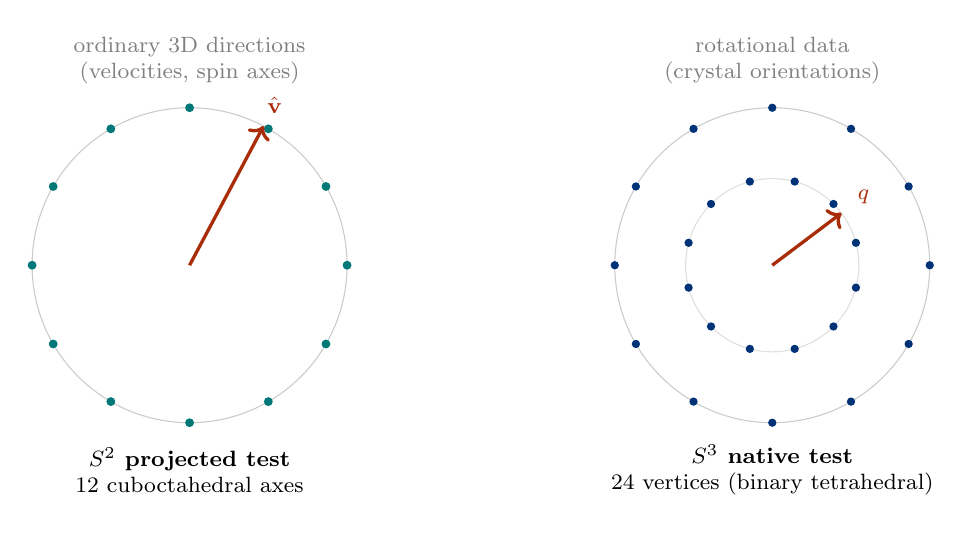
\begin{tikzpicture}[scale=1.0, font=\footnotesize]
  % Schematic cuboctahedron (2D projection) as the S^2 direction set
  \begin{scope}
    \def\r{2.0}
    \draw[gray!40] (0,0) circle (\r);
    % 12 cuboctahedron directions projected: use 12 points around / layered
    \foreach \a in {0,30,...,330} \fill[vectorteal] (\a:\r) circle (1.6pt);
    \draw[->, very thick, cruciblered] (0,0) -- (62:\r);
    \node[cruciblered] at (62:\r+0.3) {$\uvec{v}$};
    \node[align=center] at (0,-\r-0.6) {\textbf{$S^2$ projected test}\\ 12 cuboctahedral axes};
    \node[align=center, gray] at (0,\r+0.6) {ordinary 3D directions\\ (velocities, spin axes)};
  \end{scope}
  % S^3 native: schematic 24 nodes
  \begin{scope}[xshift=7.4cm]
    \def\r{2.0}
    \draw[gray!40] (0,0) circle (\r);
    \draw[gray!25] (0,0) circle (\r*0.55);
    \foreach \a in {0,30,...,330} \fill[kishblue] (\a:\r) circle (1.5pt);
    \foreach \a in {15,45,...,345} \fill[kishblue] (\a:\r*0.55) circle (1.5pt);
    \draw[->, very thick, cruciblered] (0,0) -- (37:\r*0.55);
    \node[cruciblered] at (37:\r*0.55+0.35) {$q$};
    \node[align=center] at (0,-\r-0.6) {\textbf{$S^3$ native test}\\ 24 vertices (binary tetrahedral)};
    \node[align=center, gray] at (0,\r+0.6) {rotational data\\ (crystal orientations)};
  \end{scope}
\end{tikzpicture}
\caption{Two tests, one polytope, drawn schematically (the spheres are shown as circles). Ordinary 3D
direction data is tested against the 24-cell's 3D shadow --- the 12 cuboctahedral axes on $S^2$.
Rotational data, which naturally lives on $S^3$, is tested against the 24 vertices themselves. The
engine never mixes the two, and every result is labelled with the space it was scored in.}
\end{figure}

\begin{signalbox}
\textbf{Why this is the right kind of audacious.} For the first time, the ``24'' in KishLattice is
asked to do geometric work --- to name directions, not to divide a logarithm. If the container's
geometry is real, orientations should remember it. If it is not, they will be isotropic, and the engine
will say so. Either way, the test finally engages the polytope as a polytope. That is a question worth
building an engine for, and it is one no scalar engine could ever pose.
\end{signalbox}

% ==============================================================================
\chapter{The Statistic: Directional Resonance}
% ==============================================================================

\begin{center}
\textit{The engine has two channels, mirroring the two facts a vector carries. The magnitude channel is
old --- the existing phase and period engines, unchanged. The direction channel is new, and this chapter
builds it from directional statistics in full view.}
\end{center}

\section{The Magnitude Channel (Reused, Not Reinvented)}

Every vector $\mathbf{v}_j$ has a magnitude $|\mathbf{v}_j|$, a positive scalar. On magnitudes the
programme already has two mature, fingerprinted engines. The period engine asks whether $\ln|\mathbf{v}|$
repeats with a register period; the phase engine asks whether it sits near a register node. Nothing about
the vector turn changes those statistics, and by the immutability principle the vector engine calls them
rather than reimplementing them. The magnitude channel is settled territory.

\section{The Direction Channel: Concentration on a Sphere}

The direction $\uvec{v}_j = \mathbf{v}_j / |\mathbf{v}_j|$ is a unit vector --- a point on the sphere.
The question is whether a cloud of such points is \emph{concentrated} toward the lattice axes, or spread
\emph{isotropically}. Directional statistics gives the tools exactly \cite{mardia2000, fisher1993}.

\begin{derivbox}
\textbf{The mean resultant.} For $n$ unit vectors, form the vector mean and its length:
\[
\Rbar = \frac{1}{n}\sum_{j=1}^{n}\uvec{v}_j, \qquad R = |\Rbar| \in [0,1].
\]
$R = 0$ is perfect isotropy (the arrows cancel); $R \to 1$ is perfect concentration (they align). This
is the sphere's analogue of the circular resultant on which the period engine was built
\cite{rayleigh1880}.

\textbf{The Rayleigh test for isotropy.} Under the null that directions are uniform on $S^2$, the
statistic
\[
Z = 3\,n\,R^2
\]
follows a $\chi^2$ distribution with $3$ degrees of freedom. A large $Z$ rejects isotropy. The resultant
alone, however, only detects a single preferred direction --- a \emph{dipole}. The lattice predicts
something richer: clustering toward \emph{many} axes at once.
\end{derivbox}

\begin{derivbox}
\textbf{The orientation tensor (for multi-axis and headless data).} Spin axes and polarizations are
\emph{axial}: $\uvec{v}$ and $-\uvec{v}$ are the same datum, so the resultant $\Rbar$ cancels to zero and
is useless. The correct tool is the $3\times3$ orientation tensor
\[
\mathbf{T} = \frac{1}{n}\sum_{j=1}^{n} \uvec{v}_j\,\uvec{v}_j^{\!\top},
\qquad \operatorname{tr}\mathbf{T}=1,
\]
with eigenvalues $\tau_1 \ge \tau_2 \ge \tau_3$, $\sum\tau_i = 1$. Isotropy gives
$\tau_1=\tau_2=\tau_3=\tfrac13$. A single-axis cluster drives $\tau_1 \to 1$; a girdle (plane) drives
$\tau_3 \to 0$. The Bingham and Watson distributions \cite{mardia2000} turn the eigenvalue spread into a
calibrated significance.
\end{derivbox}

\section{The Lattice-Alignment Score}

Isotropy tests ask only ``are these directions non-random?'' The lattice asks a sharper question: ``are
they non-random \emph{in the specific way the 24-cell names}?'' So the engine's headline statistic is an
alignment to the lattice axes, not a generic anisotropy.

\begin{derivbox}
Let $\{\mathbf{n}_k\}_{k=1}^{K}$ be the lattice axes ($K=12$ cuboctahedral axes on $S^2$, or $K=24$
vertices on $S^3$). For each datum define its alignment to the nearest lattice axis,
\[
a_j = \max_{k}\, \big|\,\uvec{v}_j \cdot \mathbf{n}_k\,\big| \in [0,1],
\]
and score the sample by the mean alignment $A = \tfrac{1}{n}\sum_j a_j$, reported always against the
isotropic expectation $A_{\mathrm{iso}}$ (the same quantity for uniformly random directions). The
lattice-alignment excess is $A - A_{\mathrm{iso}}$, and --- exactly as in every prior engine --- the
number that is \emph{ruled on} is not $A$ itself but its ratio to what the null produces on the same
geometry.
\end{derivbox}

\begin{figure}[H]
\centering
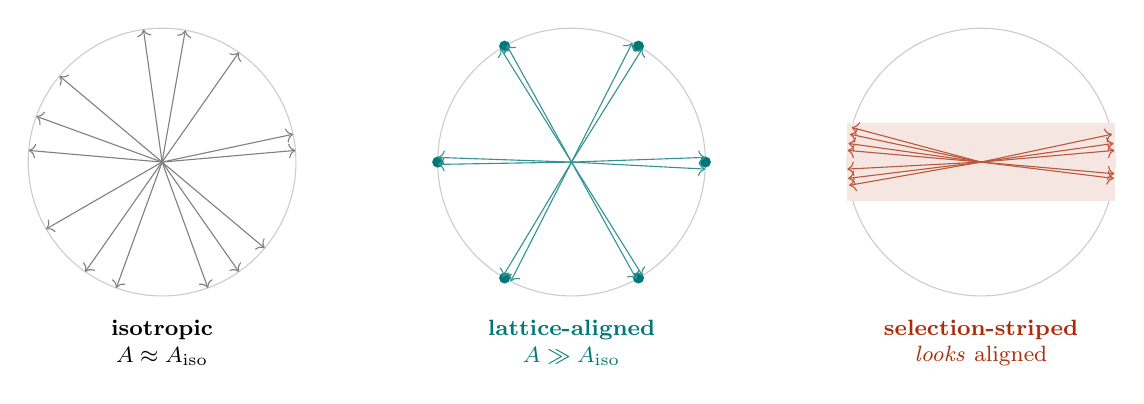
\begin{tikzpicture}[scale=1.0, font=\footnotesize]
  % isotropic
  \begin{scope}
    \def\r{1.7}
    \draw[gray!40] (0,0) circle (\r);
    \foreach \a in {12,55,98,140,175,210,250,290,320,5,80,160,235,305}
      \draw[->, gray] (0,0) -- (\a:\r);
    \node[align=center] at (0,-\r-0.6) {\textbf{isotropic}\\ $A \approx A_{\mathrm{iso}}$};
  \end{scope}
  % lattice-aligned
  \begin{scope}[xshift=5.2cm]
    \def\r{1.7}
    \draw[gray!40] (0,0) circle (\r);
    \foreach \a in {0,60,120,180,240,300} \fill[vectorteal] (\a:\r) circle (2pt);
    \foreach \a in {2,-3,58,63,119,122,181,178,239,243,299,302}
      \draw[->, vectorteal!80] (0,0) -- (\a:\r);
    \node[align=center, vectorteal] at (0,-\r-0.6) {\textbf{lattice-aligned}\\ $A \gg A_{\mathrm{iso}}$};
  \end{scope}
  % selection-striped (hazard)
  \begin{scope}[xshift=10.4cm]
    \def\r{1.7}
    \draw[gray!40] (0,0) circle (\r);
    \fill[cruciblered!12] (-\r,-0.5) rectangle (\r,0.5);
    \foreach \a in {5,-7,12,172,187,168,-5,8,175,183,190,165}
      \draw[->, cruciblered!80] (0,0) -- (\a:\r);
    \node[align=center, cruciblered] at (0,-\r-0.6) {\textbf{selection-striped}\\ \emph{looks} aligned};
  \end{scope}
\end{tikzpicture}
\caption{Three skies. Isotropic directions score at the null. Lattice-aligned directions pile toward the
preferred axes and score well above it. But a survey that only sees a band of sky (right) also piles ---
for a mundane reason that has nothing to do with the lattice. Telling the middle panel from the right
panel is the whole problem the next chapter's nulls exist to solve.}
\end{figure}

\section{The Vector Lock: Coupling the Two Channels}

The magnitude channel and the direction channel are each informative alone, but the lattice's deepest
claim is that they are \emph{coupled} --- that a vector whose magnitude lands on a register also points
along a lattice axis. A true \textbf{vector lock} is that joint event:

\[
\underbrace{\big(\,\ln|\mathbf{v}_j| \text{ near register } N\,\big)}_{\text{magnitude channel}}
\;\wedge\;
\underbrace{\big(\,a_j > \text{threshold, toward axis } k\,\big)}_{\text{direction channel}} .
\]

The vector lock is to the vector engine what the joint lock was to the 2D engine --- and, as there, the
danger is a spurious coupling produced by something other than the lattice. The instrument that disarms it
is, once again, the scramble.

% ==============================================================================
\chapter{The Nulls: Isotropy, Rotation, and the Selection Hazard}
% ==============================================================================

\begin{center}
\textit{The 2D engine taught the lesson that a null which can be fooled is worse than no null. The chaos
null was fooled by single-axis structure; only the scramble caught it. The vector engine inherits exactly
this shape of problem, and its nulls are built to the same discipline: one null to measure concentration,
one null that cannot be fooled by the shape of the survey.}
\end{center}

\section{The Isotropic Null}

The directional analogue of the chaos null: directions drawn uniformly at random on the sphere, matched in
number to the data, generated by normalising independent Gaussian vectors (the standard isotropic
construction). It answers the first question --- are the real directions more concentrated than random? ---
and it is the baseline $A_{\mathrm{iso}}$ against which the alignment excess is measured.

\begin{formbox}
\textbf{But the isotropic null can be fooled, exactly as the chaos null was.} A survey does not see the
whole sky. It sees a footprint --- a band along the Galactic plane avoided, a hemisphere favoured, a dust
mask cut out. Directions drawn from such a footprint are \emph{not} isotropic, and they will clear the
isotropic null handily --- not because the lattice structured them, but because the telescope did. This is
the directional form of the Form B hazard: structure that is real but mundane, masquerading as a lattice
signal. An engine armed only with the isotropic null would announce the shape of the survey as a discovery.
\end{formbox}

\section{The Scramble Null --- the Spine, in Direction}

As in every engine since the 2D turn, the scramble is the spine, and it is always on. In the vector engine
it takes the coupling apart:

\begin{derivbox}
\textbf{The magnitude$\leftrightarrow$direction scramble.} Shuffle which magnitude is attached to which
direction, across the sample. This destroys any coupling between how large a vector is and where it points,
while preserving \emph{both} marginals exactly --- the distribution of magnitudes is untouched, and so is
the distribution of directions, footprint and all.
\end{derivbox}

The consequence is precisely the one that redeemed the scramble in two dimensions. A survey footprint lives
entirely in the direction marginal; the scramble preserves it. So if an apparent vector lock is really just
``this anisotropic footprint happens to overlap the lattice axes,'' the scramble leaves it fully intact and
the real-to-scramble ratio sits at unity. Only a \emph{genuine coupling} --- magnitudes on registers that
also point along lattice axes, bound together --- is broken by the shuffle. The scramble cannot be fooled by
the shape of the sky, because the shape of the sky survives it.

\section{The Rotation Null --- Is the Frame Special?}

The vector engine adds one null the scalar engines never needed, because direction has something magnitude
does not: a \emph{frame}. The lattice names specific axes; a real lattice signal should be aligned to
\emph{those} axes, not merely concentrated in some arbitrary direction.

\begin{derivbox}
\textbf{The random-rotation null.} Apply a uniformly random global rotation $\mathbf{Q}\in SO(3)$ (or $SO(4)$
on $S^3$) to the entire set of lattice axes $\{\mathbf{n}_k\}$, leaving the data fixed, and recompute the
alignment $A$. Repeat over many random frames to build the distribution of $A$ under ``the lattice axes point
nowhere in particular.'' A real signal clears this null: the data aligns to the \emph{true} lattice frame far
better than to a random one. A generic anisotropy (a dipole, a footprint) does not care which frame you pick,
so it does not clear it.
\end{derivbox}

\begin{signalbox}
\textbf{Three nulls, three questions, by design.}
\begin{description}
  \item[Isotropic null] --- is the sky non-random at all? (Can be fooled by the survey footprint.)
  \item[Rotation null] --- is the alignment specific to the \emph{lattice} frame, not just any frame?
  \item[Scramble null] --- is the magnitude$\leftrightarrow$direction coupling real, or an overlap of
        independent marginals? (The spine. Cannot be fooled by the footprint.)
\end{description}
A vector lock counts only when it clears all three. The isotropic null establishes there is something to
explain; the rotation null establishes the lattice frame is special; the scramble establishes the coupling is
genuine. Any one alone is foolable; the three together are the test.
\end{signalbox}

% ==============================================================================
\chapter{How the Vector Engine Differs From All Four Before It}
% ==============================================================================

The programme now has four engines, and this is the fifth. The difference is not incremental --- it is the
first engine to leave the number line entirely.

\begin{table}[H]
\centering
\small
\renewcommand{\arraystretch}{1.25}
\begin{tabular}{@{}p{2.6cm}p{2.0cm}p{2.0cm}p{2.0cm}p{2.0cm}p{2.3cm}@{}}
\toprule
 & \textbf{1D Phase} & \textbf{1D Period} & \textbf{2D Phase} & \textbf{2D Period} & \textbf{Vector} \\
\midrule
\textbf{asks} & is a size near a node? & does a size repeat? & does a size \emph{pair} sit on a node? & does a size pair repeat jointly? & does a \emph{direction} align, and couple to size? \\
\textbf{space} & line & line & plane & torus & sphere ($S^2$ / $S^3$) \\
\textbf{data} & scalar & scalar & scalar pair & scalar pair & \textbf{vector} \\
\textbf{statistic} & node residual & circular resultant & joint cell & toroidal resultant & resultant / orientation tensor / axis alignment \\
\textbf{uses ``24'' as} & divisor & divisor & divisor & divisor & \textbf{geometry (vertices/axes)} \\
\textbf{nulls} & chaos & annular & chaos + scramble & annular + scramble & \textbf{isotropic + rotation + scramble} \\
\textbf{data appetite} & 1 wide axis & 1 wide axis & 2 wide axes, same obj. & 2 wide axes, same obj. & \textbf{directions --- abundant} \\
\bottomrule
\end{tabular}
\caption{The five engines. The vector engine is the first to leave the line for the sphere, the first whose
datum is a vector rather than a scalar, the first to use the number 24 as a set of directions rather than a
divisor, and the first whose data is plentiful rather than scarce. It adds two nulls the scalar engines never
needed --- the rotation null (a frame question) and the isotropic null (a concentration question) --- while
keeping the scramble as the spine.}
\end{table}

\begin{warningbox}
\textbf{The continuity that matters.} For all its novelty, the vector engine keeps the three commitments that
define every KishLattice instrument. The scramble null is the spine and is never tunable off. The resolution
and significance criteria are re-derived for the new space before any data is scored. And every gate must be
shown to \textsc{fail} on a fixture built to fail it before it is trusted to \textsc{pass}. The engine is new;
the discipline is not.
\end{warningbox}

% ==============================================================================
\chapter{Targets: What We Will Point It At}
% ==============================================================================

\begin{center}
\textit{Numbers up front, as always. The vector engine's targets are chosen for abundant, well-characterised
directional data and for one more thing the scalar targets never had: each is a standing question in its own
field about whether directions are truly isotropic --- the exact question a null-first directional auditor is
built to answer.}
\end{center}

\begin{table}[H]
\centering
\small
\renewcommand{\arraystretch}{1.3}
\begin{tabular}{@{}p{3.0cm}p{2.3cm}p{1.4cm}p{2.0cm}p{4.0cm}@{}}
\toprule
\textbf{Target} & \textbf{source} & \textbf{$n$} & \textbf{space} & \textbf{directional observable / hazard} \\
\midrule
Stellar space velocities & Gaia DR3 & $\sim10^6$ & $S^2$ & 3D velocity direction; hazard: disk/footprint anisotropy \\
Galaxy spin axes & SDSS, DESI & $\sim10^5$ & $S^2$ axial & spin-axis alignment (a standing, contested claim) \\
CMB polarization angles & Planck & map & $S^2$ axial & low-$\ell$ alignment (the ``axis of evil'' anomaly) \\
Pulsar spin--velocity & ATNF & $\sim10^2$ & $S^2$ & known kick alignment --- a positive-control class \\
Crystal orientations & materials DBs & $\sim10^5$ & $S^3$ & native 24-cell test; hazard: preferred growth axes \\
\bottomrule
\end{tabular}
\caption{Candidate vector targets. Unlike the scalar survey, the limiting quantity is not sample size --- it
is systematic anisotropy, named in the last column for each. The pulsar spin--velocity alignment is listed
deliberately as a \emph{known} real alignment: a class the engine must recover, or it is not trustworthy on
the cases where the answer is unknown.}
\end{table}

\begin{geobox}
\textbf{Why these, and in what order.} The pulsar spin--velocity alignment is a real, published,
non-lattice alignment --- so it is the field's gift of a positive control: a genuine directional signal the
engine must detect to prove it can. The CMB low-multipole alignment (the ``axis of evil'') is a standing
anomaly in cosmology that has never been weighed by a null-first directional auditor built against selection
and look-elsewhere from the start --- precisely our kind of question. Galaxy spin alignment is a decades-old,
still-contested claim, drowning in selection concerns --- again our kind of question. Crystal orientations are
the one target that engages the 24-cell \emph{natively} on $S^3$, with abundant data and a clean frame. Gaia
velocities are the largest and cleanest sample, and the natural first light on real data.
\end{geobox}

\begin{warningbox}
\textbf{The honest expectation, filed in advance as always.} The vector engine may find nothing --- just as
the scalar engines mostly found nothing. Physical directions may be isotropic with respect to the 24-cell, the
rotation null may show no special frame, and the scramble may destroy every apparent coupling. That is a
possible and acceptable outcome, and because the data is abundant it will be a \emph{clean} null --- a real
verdict, not the resolution-limited shrug that the starved scalar pairs could only give. If directions do
cluster on the lattice axes and survive all three nulls, it will be the first thing the programme has found
that no scalar engine could reach, and it will have engaged the 24-cell as geometry for the first time. Either
way, the answer is earned.
\end{warningbox}

% ==============================================================================
\chapter{Pre-Registrations for the Vector Engine}
% ==============================================================================

Filed before a line of engine code, under the programme's standing law. The built engine will be judged
against this list, and any departure from it will be reported as such.

\begin{predictionbox}
\textbf{Standing pre-registrations, Volume 15.}
\begin{enumerate}
    \item \textbf{Immutable from the scalar engines.} The direction channel is new code with its own
          fingerprint; the magnitude channel \emph{calls} the existing phase/period engines unchanged.
    \item \textbf{The scramble null (magnitude$\leftrightarrow$direction) wired in from the first commit}, as
          the primary coupling falsifier, always on, never tunable off.
    \item \textbf{Three nulls required for any vector lock:} isotropic (concentration), rotation (frame),
          and scramble (coupling). A lock is reported only when it clears all three; clearing fewer is reported
          as exactly that.
    \item \textbf{The $S^2$ and $S^3$ tests never conflated.} Every result is labelled with the space it was
          scored in and the axis set used (12 cuboctahedral axes, or 24 vertices).
    \item \textbf{Axial data handled with axial statistics.} Headless directions (spins, polarizations) are
          scored with the orientation tensor / Bingham, never with the resultant, which vanishes for axial data.
    \item \textbf{The selection function modelled or masked before scoring.} Survey footprint, Galactic-plane
          cut, and dust mask are declared per target and carried into the isotropic null, so that the baseline
          is the \emph{observed} sky, not an idealised full sphere.
    \item \textbf{A directional resolution/power criterion re-derived and published} before scoring: the sample
          size needed to detect a given alignment excess above the isotropic floor, which scales as $1/\sqrt{n}$.
          The analogue of $M/N$, stated for each target in advance.
    \item \textbf{Look-elsewhere corrected for the axis count and frame search}, analogous to the $23\times23$
          correction of the 2D engine.
    \item \textbf{A pre-registered positive control:} the pulsar spin--velocity alignment, which the engine must
          recover, filed as a required pass before any unknown target is trusted.
    \item \textbf{Synthetic calibration before real data:} a lattice-aligned set (must clear all three nulls), an
          isotropic set (must null), and a \emph{selection-striped} set planted to look aligned and required to be
          rejected by the scramble --- the directional expected-fail.
    \item \textbf{Every gate demonstrated to return \textsc{fail} on a fixture built to fail it}, before it is
          trusted to \textsc{pass}.
    \item \textbf{Visual inspection of sky maps and sphere plots is part of the verification chain}, not a
          presentation step --- the directional analogue of the 2D heatmap rule.
\end{enumerate}
\end{predictionbox}

% ==============================================================================
\chapter{What We Hope To See --- and What We Will Have Either Way}
% ==============================================================================

\begin{signalbox}
If directions cluster on the 24-cell's axes and survive the isotropic, rotation, and scramble nulls together,
it will be the first positive the programme has ever produced that no scalar engine could reach --- and the
first evidence that engages the container as a geometric object rather than a number in a formula. It would be
extraordinary, and it would have passed the hardest test the programme knows how to build.
\end{signalbox}

\begin{nullbox}
And if they do not --- if physical orientations are isotropic with respect to the lattice, the frame is not
special, and the scramble destroys every coupling --- then we will have established that cleanly, on abundant
data, with a real verdict rather than a resolution-limited silence. We will say so as plainly as we have said
every null before it. A clean null on a million vectors is worth more than a hopeful signal on forty-three.
\end{nullbox}

Either way, the programme ends this volume with something it did not have before: an instrument that reads
\emph{vectors}, not just scalars --- the most adaptable tool for consuming data lakes the programme has built.
Across fifteen volumes the toolkit has grown from a single-scalar comb to a matched pair of scalar engines, to
a matched pair of surface engines, and now to an engine that measures direction itself. Whatever the 24-cell
turns out to be, the instruments for asking are public, fingerprinted, and permanent --- and each one can say
no.

\begin{figure}[H]
\centering

\includegraphics[width=\textwidth]{Title/Jungle_Trek.png}
\caption{We built engines that measure how large things are. Now we build one that measures where they point. The
container, if it is real, has a shape --- and a compass is the instrument that feels for a shape in the
directions of things. --Timothy John Kish}
\label{fig:Jungle_Trek}
\end{figure}

% ==============================================================================
\chapter*{References}
\addcontentsline{toc}{chapter}{References}
% ==============================================================================

\section*{The KishLattice Series}

All volumes are published open-access with full data, configuration, and engine fingerprints. Every
pre-registration listed below was filed prior to the run it governs.

\begin{itemize}
    \item Kish, T.~J. (2026). \textit{Holographic Resonance: The Geometry of a Quantized Universe}
          (Vol.~1). Zenodo. \url{https://doi.org/10.5281/zenodo.18209530}
    \item Kish, T.~J. et al.\ (2026). \textit{The Geometric Neutron} (Vol.~2).
          Zenodo. \url{https://doi.org/10.5281/zenodo.18217119}
    \item Kish, T.~J. et al.\ (2026). \textit{The Geometric Architecture of Matter} (Vol.~3).
          Zenodo. \url{https://doi.org/10.5281/zenodo.18217226}
    \item Kish, T.~J. et al.\ (2026). \textit{The Geometric Architecture of Life} (Vol.~4).
          Zenodo. \url{https://doi.org/10.5281/zenodo.18976975}
    \item Kish, T.~J. et al.\ (2026). \textit{The Geometric Architecture of Unification} (Vol.~5).
          Zenodo. \url{https://doi.org/10.5281/zenodo.19009634}
    \item Kish, T.~J. et al.\ (2026). \textit{The Harmonic Expansion of the Unified Lattice}
          (Vol.~6). Zenodo. \url{https://doi.org/10.5281/zenodo.19493376}
    \item Kish, T.~J. et al.\ (2026). \textit{The Sovereign Resonance} (Vol.~7).
          Zenodo. \url{https://doi.org/10.5281/zenodo.19559860}
    \item Kish, T.~J. et al.\ (2026). \textit{Unbounded Luminosity} (Vol.~8).
          Zenodo. \url{https://doi.org/10.5281/zenodo.19622632}
    \item Kish, T.~J. et al.\ (2026). \textit{KishLattice Geometric Harmonic Spectroscopy: The First
          Survey of a New Field} (Vol.~9). Zenodo. \url{https://doi.org/10.5281/zenodo.19935603}
    \item Kish, T.~J. et al.\ (2026). \textit{The Deep Survey} (Vol.~10).
          Zenodo. \url{https://doi.org/10.5281/zenodo.20279208}
    \item Kish, T.~J. et al.\ (2026). \textit{The Structure That Locks} (Vol.~11).
          Zenodo. \url{https://doi.org/10.5281/zenodo.20587180}
    \item Kish, T.~J. et al.\ (2026). \textit{The Crucible --- The Instrument Audit, Five Artifact
          Forms, and the Resolution Criterion} (Vol.~12).
          Zenodo. \url{https://doi.org/10.5281/zenodo.22416330}
    \item Kish, T.~J. et al.\ (2026). \textit{The Aperture --- Dynamic Range as the Hidden Variable}
          (Vol.~13). Zenodo. \url{https://doi.org/10.5281/zenodo.22851850}
          \\ \textit{Direct predecessor. Pre-registers both lake rebuilds closed in Chapters 1--2 of
          the present volume, and carries the resolution criterion $M/N > 2.67$ used throughout.}
\end{itemize}

\section*{Pre-Registrations and Supporting Papers}

\begin{itemize}
    \item Kish, T.~J. et al.\ (2026). \textit{Noise Does Not Lock --- A Comprehensive Empirical
          Response to Skeptical Challenges to KishLattice Geometric Harmonic Spectroscopy}.
          Zenodo. \url{https://doi.org/10.5281/zenodo.20585516}
          \\ \textit{Source of the Grid-Phase Locking Theorem and of the scramble-null analysis
          (Erratum 1) on which Chapters 4--6 turn.}
    \item Kish, T.~J. et al.\ (2026). \textit{Master Equation of the Kish Lattice Theory --- The
          Rosetta Atlas}. Zenodo. \url{https://doi.org/10.5281/zenodo.18235735}
          \\ \textit{Source of the lattice energy expression and of the definition of $f$ carried
          forward from Volume 13.}
    \item Kish, T.~J. et al.\ (2026). \textit{Volume 13 --- Pre-Registration P13.1--P13.6}.
          Zenodo. \textit{Carries the resolution census and the two rebuild specifications upheld in
          Chapters 1--2.}
    \item Internal memorandum AM-15-01 (2026). \textit{Vol 15 Direction: The General Falsifier ---
          Bode's Law, the Exoplanet Hand-off, and the $\kgeo$ Refactor; the Dimensional Ladder and
          the Vector Engine.} KishLattice 16$\pi$ Initiative LLC.
          \\ \textit{Records the go/no-go discipline of the nuclear probe in Chapter 7 and the
          dimensional-ladder reasoning deferring the 3D scalar engine in favour of the vector engine.}
\end{itemize}

\section*{Repository and Project Resources}

\begin{itemize}
    \item Kish, T.~J. \textit{Holographic Resonance: The Geometry of a Quantized Universe} --- engine
          source, configurations, audit scripts, and run receipts. GitHub.
          \url{https://github.com/TimothyKish/Holographic-Resonance-The-Geometry-of-a-Quantized-Universe}
    \item KishLattice 16$\pi$ Initiative LLC. \url{https://www.kishlattice.com}
\end{itemize}

\noindent The scripts released with this volume reproduce each table and verdict from the published
lakes, and each aborts rather than substituting a value when a required field is absent:

\begin{itemize}
    \item \texttt{kish\_lake\_io.py} --- strict field contract; recursive resolver; coverage reporting.
    \item \texttt{build\_s2\_kinematics\_rebuild.py}, \texttt{promote\_rebuild.py} --- the \texttt{s2}
          covariance rebuild of Chapter 1 ($5\sigma$ parallax and covariance-propagated proper-motion
          gates; DR3 zero-point; computed $M/N$).
    \item \texttt{periodogram2d.py}, \texttt{phase\_lock2d.py} --- the two 2D engines (Chapters 5--6);
          the scramble null is always on; the census compares best-of-grid real against
          best-of-grid scramble.
    \item \texttt{build\_velocity\_luminosity\_lake.py}, \texttt{support2d.py} --- the maiden-voyage
          lake and support audit of Chapter 6.
    \item \texttt{probe\_nuclear\_runway.py} --- the go/no-go feasibility probe of Chapter 7; measures
          span and gate on each axis of the strict join and scores nothing.
    \item \texttt{make\_synthetic\_lakes.py} --- the four permanent 2D control lakes (seed-fixed,
          regenerable byte-for-byte).
\end{itemize}

\section*{Primary Data Sources --- Vol 14}

\begin{itemize}
    \item \textbf{Gaia Collaboration} (2023). Gaia Data Release 3. VizieR catalogue I/355.
          \\ \textit{Source of the \texttt{s2} stellar-kinematics rebuild (Chapter 1) and of the
          velocity$\times$luminosity lake (Chapter 6, $n = 83{,}155$ promoted pairs).}
    \item \textbf{LIGO/Virgo/KAGRA Collaboration}, Gravitational-Wave Transient Catalogue GWTC-3,
          with \texttt{pyRing} ringdown posteriors. \url{https://www.gw-openscience.org/}
          \\ \textit{Source of the \texttt{l1\_gwtc} rebuild (Chapter 2); measured $f_{220}$,
          $n = 21$ Kerr-consistent events.}
    \item \textbf{NNDC / IAEA nuclear data} --- NuDat and the NUBASE2020 evaluation.
          \url{https://www.nndc.bnl.gov/nudat3/}
          \\ \textit{Source of the \texttt{Q5} decay lake (half-life axis) of the Chapter 7 probe.}
    \item \textbf{Atomic Mass Evaluation (AME2020)}, Kondev et al.
          \\ \textit{Source of the \texttt{Q4} nuclear lake (decay-energy axis) of the Chapter 7
          probe; strict join yielded 43 matched nuclides.}
    \item CODATA 2022 recommended values of the fundamental physical constants.
          \url{https://physics.nist.gov/cuu/Constants/}
\end{itemize}

\section*{Primary Data Sources --- Vol 15 Targets}

\begin{itemize}
    \item \textbf{Gaia Collaboration} (2023). Gaia Data Release 3. VizieR catalogue I/355.
          \\ \textit{Stellar space-velocity directions; the largest and cleanest $S^2$ target.}
    \item \textbf{Sloan Digital Sky Survey / DESI.} \url{https://www.sdss.org/} ; \url{https://www.desi.lbl.gov/}
          \\ \textit{Galaxy spin-axis orientations; axial $S^2$ data for the spin-alignment question.}
    \item \textbf{Planck Collaboration} (2020). Planck 2018 results.
          \textit{Astronomy \& Astrophysics}, 641, A6.
          \\ \textit{CMB polarization; the low-multipole alignment anomaly.}
    \item \textbf{ATNF Pulsar Catalogue.} \url{https://www.atnf.csiro.au/research/pulsar/psrcat/}
          \\ \textit{Pulsar spin and proper-motion directions; the pre-registered positive control.}
    \item \textbf{Materials orientation databases} (e.g.\ MP, EBSD repositories).
          \\ \textit{Crystallographic orientations; the native $S^3$ test against the 24 vertices.}
\end{itemize}

% ==============================================================================
\begin{thebibliography}{99}
\addcontentsline{toc}{section}{Scientific References}
\section*{Scientific References}

\bibitem{rayleigh1880v14}
Rayleigh, Lord (J.~W. Strutt) (1880).
On the resultant of a large number of vibrations of the same pitch and of arbitrary phase.
\textit{Philosophical Magazine}, 10(60), 73--78.
\textit{(The circular resultant $R$ on which the period engines --- one- and two-dimensional --- are
built.)}

\bibitem{gross2010v14}
Gross, E., \& Vitells, O. (2010).
Trial factors for the look elsewhere effect in high energy physics.
\textit{European Physical Journal C}, 70, 525--530.
\textit{(Basis of the look-elsewhere correction. In two dimensions the scan covers
$23\times23 = 529$ register pairs, which the census null corrects by comparing best-of-grid real
against best-of-grid scramble.)}

\bibitem{bracewell2000v14}
Bracewell, R.~N. (2000).
\textit{The Fourier Transform and Its Applications} (3rd ed.). McGraw-Hill, Boston.
\textit{(Finite-aperture spectral leakage; the resolution criterion $M/N > 2.67$ that both axes of a
2D pair must independently satisfy.)}

\bibitem{kondev2021v14}
Kondev, F.~G., Wang, M., Huang, W.~J., Naimi, S., \& Audi, G. (2021).
The NUBASE2020 evaluation of nuclear physics properties.
\textit{Chinese Physics C}, 45, 030001.
\textit{(Evaluated half-lives underlying the \texttt{Q5} decay lake: full-lake effective span
$31.8$ decades, compressed to $16.4$ decades on the strict 43-nuclide join of Chapter 7. Companion
to the AME2020 mass evaluation supplying the decay-energy axis.)}

\bibitem{berti2006v14}
Berti, E., Cardoso, V., \& Will, C.~M. (2006).
On gravitational-wave spectroscopy of massive black holes with the space interferometer LISA.
\textit{Physical Review D}, 73, 064030.
\textit{(Fit to the fundamental $\ell=m=2$ Kerr quasinormal mode, used to invert spin from $f_{220}$
and remnant mass in the Kerr-consistency gate of Chapter 2.)}

\bibitem{gwtc3v14}
Abbott, R., et al.\ (LIGO Scientific, Virgo and KAGRA Collaborations) (2023).
GWTC-3: Compact binary coalescences observed during the second part of the third observing run.
\textit{Physical Review X}, 13, 041039.
\textit{(The ringdown catalogue rebuilt in Chapter 2; the O4/O5 runs are the deferred data of the
strong-field test.)}

\bibitem{gaia2023v14}
Gaia Collaboration (2023).
Gaia Data Release 3: Summary of the content and survey properties.
\textit{Astronomy \& Astrophysics}, 674, A1.
\textit{(The astrometric and photometric source of the \texttt{s2} rebuild and the
velocity$\times$luminosity lake.)}

\bibitem{tifft1976v14}
Tifft, W.~G. (1976).
Discrete states of redshift and galaxy dynamics I.
\textit{Astrophysical Journal}, 206, 38--56.
\textit{(The closest historical precedent to a cross-domain periodicity survey; later attributed to
selection effects and limited dynamic range --- the second of which closes the 2D survey here.)}

\bibitem{sornette1998v14}
Sornette, D. (1998).
Discrete scale invariance and complex dimensions.
\textit{Physics Reports}, 297(5), 239--270.
\textit{(The established physics of log-periodic structure; the near-node and scramble disciplines of
this volume apply to that literature equally.)}

\bibitem{mardia2000}
Mardia, K.~V., \& Jupp, P.~E. (2000).
\textit{Directional Statistics}. Wiley, Chichester.
\textit{(The reference for the resultant on the sphere, the orientation tensor, and the Bingham and Watson
distributions for axial data --- the full statistical basis of the direction channel.)}

\bibitem{fisher1993}
Fisher, N.~I. (1993).
\textit{Statistical Analysis of Circular Data}. Cambridge University Press.
\textit{(Companion treatment; the resolution/power arguments adapted to the directional resolution criterion
of VP15.7.)}

\bibitem{rayleigh1880}
Rayleigh, Lord (J.~W. Strutt) (1880).
On the resultant of a large number of vibrations of the same pitch and of arbitrary phase.
\textit{Philosophical Magazine}, 10(60), 73--78.
\textit{(The resultant $R$ --- here lifted from the circle to the sphere as $\Rbar$, with the Rayleigh test
$Z = 3nR^2$.)}

\bibitem{watson1965}
Watson, G.~S. (1965).
Equatorial distributions on a sphere.
\textit{Biometrika}, 52(1/2), 193--201.
\textit{(The Watson distribution for axial data; basis of the spin-axis and polarization tests.)}

\bibitem{bingham1974}
Bingham, C. (1974).
An antipodally symmetric distribution on the sphere.
\textit{Annals of Statistics}, 2(6), 1201--1225.
\textit{(The Bingham distribution; the orientation-tensor eigenvalue test for multi-axis clustering.)}

\bibitem{gross2010}
Gross, E., \& Vitells, O. (2010).
Trial factors for the look elsewhere effect in high energy physics.
\textit{European Physical Journal C}, 70, 525--530.
\textit{(Basis of the look-elsewhere correction over the axis count and the rotation-frame search, VP15.8.)}

% --- Polytope geometry: the 24-cell ---

\bibitem{coxeter1973}
Coxeter, H.~S.~M. (1973).
\textit{Regular Polytopes} (3rd ed.). Dover, New York.
\textit{(The 24-cell: 24 vertices, self-dual, symmetry group $F_4$ of order 1152; the cuboctahedral and
rhombic-dodecahedral projections into three dimensions used for the $S^2$ test.)}

\bibitem{conwaysloane1999}
Conway, J.~H., \& Sloane, N.~J.~A. (1999).
\textit{Sphere Packings, Lattices and Groups} (3rd ed.). Springer, New York.
\textit{(The $D_4$ root system and the unit-quaternion / binary-tetrahedral form of the 24-cell vertices ---
the two coordinate presentations of Chapter 3.)}

\bibitem{dutour2003}
Dutour Sikiri\'c, M., \& Deza, M. (2003).
The hypermetric cone and polytopes of the 24-cell.
\textit{(Context for the projections of the 24-cell used to define the $S^2$ axis set.)}

% --- Isotropy: the questions the engine joins ---

\bibitem{landau2016}
Land, K., \& Magueijo, J. (2005).
The axis of evil.
\textit{Physical Review Letters}, 95, 071301.
\textit{(The low-multipole CMB alignment anomaly; a standing directional question the vector engine is built
to weigh against selection and look-elsewhere.)}

\bibitem{planck2020iso}
Planck Collaboration (2020).
Planck 2018 results. VII. Isotropy and statistics of the CMB.
\textit{Astronomy \& Astrophysics}, 641, A7.
\textit{(The authoritative isotropy analysis; the selection and masking discipline VP15.6 adopts.)}

\bibitem{trujillo2006}
Trujillo, I., Carretero, C., \& Patiri, S.~G. (2006).
Detection of the effect of cosmological large-scale structure on the orientation of galaxies.
\textit{Astrophysical Journal Letters}, 640, L111--L114.
\textit{(Representative of the contested galaxy spin-alignment literature --- real claims, heavy selection
concerns; the kind of question a null-first directional auditor is meant for.)}

\bibitem{noutsos2012}
Noutsos, A., Schnitzeler, D.~H.~F.~M., Keane, E.~F., Kramer, M., \& Johnston, S. (2012).
Pulsar spin--velocity alignment: kinematic ages, birth periods and braking indices.
\textit{Monthly Notices of the Royal Astronomical Society}, 423, 2736--2752.
\textit{(The pulsar spin--velocity alignment --- a real, published directional signal; the pre-registered
positive control of VP15.9.)}

\bibitem{gaia2023}
Gaia Collaboration (2023).
Gaia Data Release 3: Summary of the content and survey properties.
\textit{Astronomy \& Astrophysics}, 674, A1.
\textit{(The stellar space-velocity sample; the first-light real target.)}

\bibitem{sornette1998}
Sornette, D. (1998).
Discrete scale invariance and complex dimensions.
\textit{Physics Reports}, 297(5), 239--270.
\textit{(The magnitude channel's log-periodic basis, reused unchanged from the scalar engines.)}

\end{thebibliography}

% =============================================================================
% Vol 14 -- DROP-IN APPENDIX A : The Filter Ablation
% =============================================================================

\appendix

% ==============================================================================
\chapter{The Filter Ablation: What Each Guard Contributes to the Verdict}
% ==============================================================================

\begin{center}
\textit{The 2D engines carry three tunable form filters, built as toggles on purpose so that their
contribution could be measured rather than assumed. This appendix measures it. We run the full
factorial --- every on/off combination of the three filters --- against lakes with known answers, and
report exactly how much each guard moves the verdict. The result is clean, a little surprising, and it
closes the 2D engine with a number instead of a claim.}
\end{center}

\section{The Point of the Ablation}

A filter that is always on is a filter whose contribution you cannot see. From the first commit the
2D engines exposed their artifact filters as switches --- \texttt{common\_support}, \texttt{scale\_flag},
and the \texttt{resolution\_gate} --- precisely so that we could run the engine with each one on, then
off, and read the difference directly off the census. The question this appendix answers is empirical
and specific: \emph{how much does each form-artifact guard actually contribute to the final verdict,
and do any of them compound?}

\begin{warningbox}
\textbf{Which guards are toggles, and which are not.} Of the programme's five artifact forms, only three
correspond to a tunable filter. The scramble null --- the defence against Form B (mundane correlation)
and single-axis structure --- is the \emph{spine}: always on, never a toggle, and therefore not ablated.
Its contribution is read in \emph{every} cell of the experiment as the real-to-scramble ratio itself.
Form A (the transform artifact) is the open gate (\texttt{FORM\_A\_UNCLEARED}), a theory question, not a
filter. So the factorial is over exactly the three tunable guards.
\end{warningbox}

\begin{table}[H]
\centering
\small
\begin{tabular}{@{}p{3.2cm}p{5.9cm}p{4.6cm}@{}}
\toprule
\textbf{toggle (default on; \texttt{--no-X} off)} & \textbf{targets} & \textbf{role} \\
\midrule
\texttt{common\_support} & Form D --- null-support / floor mismatch & per-coordinate support correction \\
\texttt{scale\_flag}     & Form C --- scale degeneracy / preprocessing & per-axis rescaling flag \\
\texttt{resolution\_gate}& the $\MN > 2.67$ criterion & refuses unresolvable register pairs \\
\midrule
\textit{scramble null}   & \textit{Form B + single-axis} & \textit{the spine --- always on, not a toggle} \\
\bottomrule
\end{tabular}
\caption{The three tunable guards and the always-on spine. The ablation toggles the top three; the
scramble is read in every run.}
\end{table}

\section{The Design}

Three binary toggles give $2^3 = 8$ combinations per engine. The full factorial captures each filter's
individual effect \emph{and} every pairwise and triple interaction, so compounding is visible if it
exists. Each combination was scored, through the identical pipeline, against the four synthetic control
lakes (where the ground truth is known by construction) and the real velocity$\times$luminosity lake.

\begin{table}[H]
\centering
\small
\begin{tabular}{@{}cccl@{}}
\toprule
\texttt{common\_support} & \texttt{scale\_flag} & \texttt{resolution\_gate} & reads \\
\midrule
on  & on  & on  & baseline (what Chapters 5--6 reported) \\
off & on  & on  & Form D alone removed \\
on  & off & on  & Form C alone removed \\
on  & on  & off & resolution gate alone removed \\
off & off & on  & C $+$ D compounding \\
off & on  & off & D $+$ gate compounding \\
on  & off & off & C $+$ gate compounding \\
off & off & off & all guards removed --- raw statistic \\
\bottomrule
\end{tabular}
\caption{The $2^3$ factorial. The harness \texttt{ablate\_2d.py} drives the real pipeline as a
subprocess under each combination, with the scramble null on throughout, and tabulates the
best-of-grid real-to-scramble ratio per lake.}
\end{table}

\section{The Results}

Numbers up front, exactly as returned. The striking feature is visible before any interpretation: the
ratio column does not move.

\begin{table}[H]
\centering
\small
\begin{tabular}{@{}l ccc rrr@{}}
\toprule
\multicolumn{4}{c}{\textbf{2D PERIOD engine}} & \multicolumn{3}{c}{\textbf{best-of-grid ratio}} \\
\cmidrule(lr){1-4}\cmidrule(lr){5-7}
combo & CS & SF & RG & \texttt{jointlock} & \texttt{noise} & \texttt{vel$\times$lum} \\
\midrule
111 & Y & Y & Y & $16.91$ & $1.09$ & $0.88$ \\
110 & Y & Y & -- & $16.91$ & $1.09$ & $0.88$ \\
101 & Y & -- & Y & $16.91$ & $1.09$ & $0.88$ \\
011 & -- & Y & Y & $16.91$ & $1.09$ & $0.88$ \\
100 & Y & -- & -- & $16.91$ & $1.09$ & $0.88$ \\
010 & -- & Y & -- & $16.91$ & $1.09$ & $0.88$ \\
001 & -- & -- & Y & $16.91$ & $1.09$ & $0.88$ \\
000 & -- & -- & -- & $16.91$ & $1.09$ & $0.88$ \\
\midrule
\multicolumn{4}{r}{\textbf{spread across all 8:}} & $\mathbf{0.00}$ & $\mathbf{0.00}$ & $\mathbf{0.00}$ \\
\bottomrule
\end{tabular}
\caption{Period engine ablation. The best-of-grid ratio is identical in all eight combinations, to the
precision reported. CS~=~common\_support, SF~=~scale\_flag, RG~=~resolution\_gate.}
\end{table}

\begin{table}[H]
\centering
\small
\begin{tabular}{@{}l ccc rrrrr@{}}
\toprule
\multicolumn{4}{c}{\textbf{2D PHASE engine}} & \multicolumn{5}{c}{\textbf{best-of-grid ratio}} \\
\cmidrule(lr){1-4}\cmidrule(lr){5-9}
combo & CS & SF & RG & \texttt{formB} & \texttt{jointlock} & \texttt{noise} & \texttt{oneaxis} & \texttt{vel$\times$lum} \\
\midrule
111 & Y & Y & Y & $1.00$ & $2.24$ & $0.97$ & $0.98$ & $1.00$ \\
\multicolumn{4}{@{}l}{\textit{all other 7 combos}} & $1.00$ & $2.24$ & $0.97$ & $0.98$ & $1.00$ \\
\midrule
\multicolumn{4}{r}{\textbf{spread across all 8:}} & $\mathbf{0.00}$ & $\mathbf{0.00}$ & $\mathbf{0.00}$ & $\mathbf{0.00}$ & $\mathbf{0.00}$ \\
\bottomrule
\end{tabular}
\caption{Phase engine ablation. Every lake returns an identical ratio in all eight combinations. The
planted lock survives (2.24); the correlation ridge, pure noise, single-axis artifact, and the real
lake all sit at the floor --- and none of that depends on the tunable filters.}
\end{table}

\begin{figure}[H]
\centering
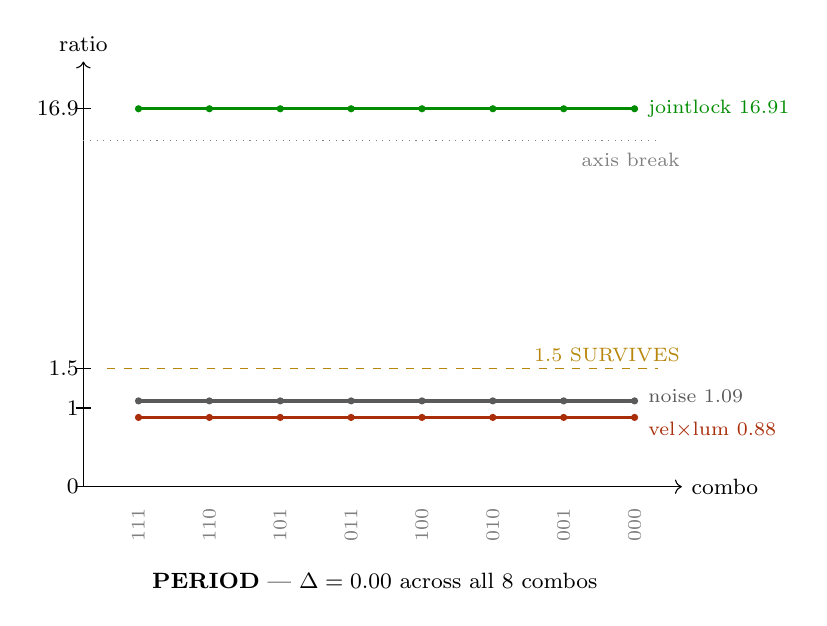
\begin{tikzpicture}[scale=1.0, font=\footnotesize]
  % ---- PERIOD panel ----
  \begin{scope}
    \draw[->] (0,0) -- (0,5.4) node[above] {\footnotesize ratio};
    \draw[->] (0,0) -- (7.6,0) node[right] {\footnotesize combo};
    % y ticks (linear-ish compressed: 0,1,1.5 near bottom, 16.91 near top via a break)
    \foreach \y/\lab in {0.0/0, 1.0/1, 1.5/1.5, 4.8/16.9} \draw (-0.1,\y) -- (0.1,\y) node[left=1pt] {\lab};
    \draw[dotted, gray] (0,4.4) -- (7.3,4.4); % break hint
    \node[gray, right] at (6.2,4.15) {\scriptsize axis break};
    % x combos
    \foreach \x/\lab in {0.7/111,1.6/110,2.5/101,3.4/011,4.3/100,5.2/010,6.1/001,7.0/000}
      \node[rotate=90, anchor=east, gray] at (\x,-0.15) {\scriptsize \lab};
    % SURVIVES threshold
    \draw[dashed, goldseal] (0.3,1.5) -- (7.3,1.5);
    \node[goldseal, right] at (5.6,1.68) {\scriptsize 1.5 SURVIVES};
    % jointlock flat line at 4.8 (represents 16.91 above the break)
    \draw[very thick, signalgreen] (0.7,4.8) -- (7.0,4.8);
    \foreach \x in {0.7,1.6,2.5,3.4,4.3,5.2,6.1,7.0} \fill[signalgreen] (\x,4.8) circle (1.3pt);
    \node[signalgreen, right] at (7.05,4.8) {\scriptsize jointlock 16.91};
    % noise flat line at 1.09
    \draw[very thick, formgray] (0.7,1.09) -- (7.0,1.09);
    \foreach \x in {0.7,1.6,2.5,3.4,4.3,5.2,6.1,7.0} \fill[formgray] (\x,1.09) circle (1.3pt);
    \node[formgray, right] at (7.05,1.15) {\scriptsize noise 1.09};
    % vel flat line at 0.88
    \draw[very thick, cruciblered] (0.7,0.88) -- (7.0,0.88);
    \foreach \x in {0.7,1.6,2.5,3.4,4.3,5.2,6.1,7.0} \fill[cruciblered] (\x,0.88) circle (1.3pt);
    \node[cruciblered, right] at (7.05,0.72) {\scriptsize vel$\times$lum 0.88};
    \node[align=center] at (3.7,-1.2) {\textbf{PERIOD} --- $\Delta = 0.00$ across all 8 combos};
  \end{scope}
\end{tikzpicture}
\caption{Verdict invariance (period engine; the phase engine is identical in character). Every lake's
best-of-grid ratio is a dead-flat line across all eight toggle combinations. The planted lock sits far
above the \textsc{survives} threshold; the nulls and the real lake sit at the floor; and nothing ---
not a single guard, nor any compounding of them --- moves any line. The tunable filters do not change
the verdict.}
\end{figure}

\section{Finding 1 --- The Verdict Is Invariant; the Scramble Carries It}

The headline is the flatness. Across all eight combinations, in both engines, every lake returns the
same ratio it returned with every guard on. Removing Form~D, removing Form~C, removing the resolution
gate, and removing all three at once change the census verdict by $0.00$.

\begin{signalbox}
\textbf{The scramble null carries the entire verdict.} The three tunable filters contribute nothing to
the final number on these lakes. The one defence that is \emph{not} a toggle --- the scramble, the spine
--- is the one that determines every outcome. This is the strongest possible statement about a
falsifier's integrity: the verdict rests on the single component that can never be switched off, and is
robust to every knob that can.
\end{signalbox}

There is a clean reason for this, and it is worth writing down because it is structural, not accidental.

\begin{derivbox}
The census statistic is a \emph{ratio} of two best-of-grid powers,
\[
\rho \;=\; \frac{\displaystyle\max_{(N_1,N_2)\in\mathcal{G}} P_{\mathrm{real}}(N_1,N_2)}
                 {\displaystyle\max_{(N_1,N_2)\in\mathcal{G}} P_{\mathrm{scr}}(N_1,N_2)} .
\]
A filter acts in one of two ways: the resolution gate restricts the eligible grid,
$\mathcal{G}\to\mathcal{G}_f$; the support and scale corrections reweight the per-pair power,
$P\to P_f$. Crucially, every filter is applied \emph{identically to the real lake and to its scramble},
because the scramble passes through the entire pipeline as a sibling lake. So both numerator and
denominator are transformed by the same $f$:
\[
\rho_f \;=\; \frac{\displaystyle\max_{\mathcal{G}_f} P_{f,\mathrm{real}}}
                  {\displaystyle\max_{\mathcal{G}_f} P_{f,\mathrm{scr}}} .
\]
When the winning pair survives the filter for both real and scramble --- which it does whenever the
winner is already a well-resolved, well-supported pair --- the correction multiplies top and bottom by
the same factor and the ratio is unchanged. \textbf{The filters move the floor; they do not move the
ratio of the two peaks above it.} The ablation confirms the cancellation empirically: $\Delta\rho = 0.00$.
\end{derivbox}

\begin{figure}[H]
\centering
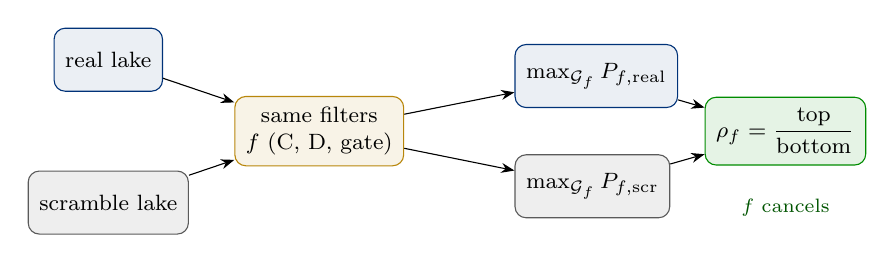
\begin{tikzpicture}[scale=1.0, font=\footnotesize, >=Stealth,
   node distance=6mm,
   b/.style={draw, rounded corners, align=center, inner sep=4pt, minimum height=8mm}]
  \node[b, fill=kishblue!8, draw=kishblue] (real) {real lake};
  \node[b, fill=formgray!10, draw=formgray, below=10mm of real] (scr) {scramble lake};
  \node[b, fill=goldseal!10, draw=goldseal, right=16mm of $(real)!0.5!(scr)$] (f) {same filters\\ $f$ (C, D, gate)};
  \node[b, fill=kishblue!8, draw=kishblue, right=14mm of f, yshift=7mm] (pr) {$\max_{\mathcal{G}_f} P_{f,\mathrm{real}}$};
  \node[b, fill=formgray!10, draw=formgray, right=14mm of f, yshift=-7mm] (ps) {$\max_{\mathcal{G}_f} P_{f,\mathrm{scr}}$};
  \node[b, fill=signalgreen!10, draw=signalgreen, right=14mm of $(pr)!0.5!(ps)$] (rho) {$\rho_f = \dfrac{\text{top}}{\text{bottom}}$};
  \draw[->] (real) -- (f); \draw[->] (scr) -- (f);
  \draw[->] (f) -- (pr); \draw[->] (f) -- (ps);
  \draw[->] (pr) -- (rho); \draw[->] (ps) -- (rho);
  \node[align=center, signalgreen!60!black, below=3mm of rho] {\scriptsize $f$ cancels};
\end{tikzpicture}
\caption{Why the filters cancel. The same filter $f$ is applied to the real lake and its scramble before
the ratio is taken. A correction that multiplies the real peak also multiplies the scramble peak, so it
divides out. The verdict is, by construction, robust to the tunable guards --- and determined by the
scramble.}
\end{figure}

\section{Finding 2 --- The Resolution Gate Governs Coverage, Not Verdict}

One toggle does change an observable quantity --- but not the one that decides anything.

\begin{table}[H]
\centering
\small
\begin{tabular}{@{}llrr@{}}
\toprule
\textbf{lake} & \textbf{resolution gate} & \textbf{pairs scored} & \textbf{ratio} \\
\midrule
\texttt{synth} lakes      & on  & $225/529$ & unchanged \\
\texttt{synth} lakes      & off & $529/529$ & unchanged \\
\texttt{velocity$\times$luminosity} & on  & $112/529$ & $0.88$ \\
\texttt{velocity$\times$luminosity} & off & $\mathbf{529/529}$ & $\mathbf{0.88}$ \\
\bottomrule
\end{tabular}
\caption{The resolution gate's only effect is coverage. Turning it off scores every pair on the grid;
the best-of-grid ratio is unchanged, because the pairs the gate removes were never going to win.}
\end{table}

\begin{signalbox}
\textbf{This strengthens the velocity$\times$luminosity null of Chapter 6.} With the gate on, only $112$
of $529$ pairs were scoreable --- and a skeptic could fairly ask whether the null was an artifact of the
gate quietly hiding the other $417$. The ablation answers that directly: with the gate \emph{off}, all
$529$ pairs are scored, and the ratio is still $0.88$. The null is not a gate artifact. It holds across
the entire register grid. The gate's role is honesty of coverage --- it refuses to report pairs the data
cannot resolve --- not suppression of a signal.
\end{signalbox}

\section{Finding 3 --- The Honest Boundary: C and D Had Nothing to Bite On}

The temptation here is to over-read Finding~1 --- to conclude the Form-C and Form-D filters are useless.
That conclusion would be wrong, and stating why is the honest close.

\begin{correctionbox}
\textbf{Zero contribution here is not zero contribution in general.} The \texttt{common\_support} and
\texttt{scale\_flag} filters are built to suppress a \emph{specific} artifact each: a floor-mismatch
concentration (Form D) and a scale-degeneracy alignment (Form C). None of the four control lakes
\emph{contains} such an artifact reaching the best-of-grid. The planted set is a true joint lock, pure
noise, a Form-B correlation ridge, and a single-axis artifact --- and the scramble already disposes of
the last two (\texttt{formB} $1.00$, \texttt{oneaxis} $0.98$). The C and D filters were handed nothing to
catch, so their measured contribution is correctly zero. This is a statement about the \emph{lakes}, not
a proof the filters never matter.
\end{correctionbox}

To test the C and D filters' protective value properly, the engine must be shown a lake that contains the
very artifact each is built to suppress --- and shown that the filter, and only the filter, removes the
spurious lock. That is a clean, bounded follow-up, and we file it as a pre-registration rather than leave
it implied.

\begin{predictionbox}
\textbf{Pre-registration (filed for the next 2D calibration pass).}
\begin{enumerate}
    \item \textbf{A Form-C planted control:} a lake with a phase-neutral rescaling of one axis chosen to
          manufacture a joint alignment. Required result: a spurious lock that \emph{survives the
          scramble} but is removed by \texttt{scale\_flag} --- the case that would prove the filter catches
          something the spine does not.
    \item \textbf{A Form-D planted control:} a lake with a large below-floor population on each axis, so
          the clamp manufactures near-node mass. Required result: a spurious lock removed by
          \texttt{common\_support} applied per-coordinate.
    \item If either filter fails to remove its planted artifact, or if the scramble already removes it
          (making the filter redundant), that is itself the reportable finding.
\end{enumerate}
\end{predictionbox}

\section{What the Ablation Closes}

\begin{nullbox}
\textbf{The empirical standing of the 2D guards, measured not asserted.} On the lakes tested --- four
controls with known answers and the one real pair --- the census verdict is invariant to all three
tunable filters ($\Delta\rho = 0.00$, both engines, all eight combinations). The scramble null, the one
component that is never a toggle, carries the verdict entirely. The resolution gate governs coverage, not
outcome, and the velocity$\times$luminosity null holds with the gate off across the full $529$-pair grid.
The Form-C and Form-D filters are confirmed inert on the current lakes, for want of a planted artifact to
suppress; their protective value is pre-registered for a dedicated calibration pass.
\end{nullbox}

This is the way the programme closes every component: with a number that could have come out otherwise.
The filters \emph{could} have moved the verdict, and we would have reported by how much. They did not, and
we report that --- along with the honest reason, and the test that would complete the picture. The 2D
engine's tunable guards are now characterised, and the spine is shown, empirically, to be exactly that.

\begin{center}
\vspace{0.5em}
\itshape
We built the filters as switches so their worth could be weighed, not assumed. Weighed, they move the
verdict by nothing --- and in moving nothing, they prove that everything rests on the one thing we never
let anyone switch off.
\vspace{0.5em}
\end{center}


% =============================================================================
% Vol 14 -- DROP-IN APPENDIX B : Formal Verification with Lean
% =============================================================================
% ==============================================================================
\chapter{Formal Verification with Lean: Certifying the Instrument}
% ==============================================================================

\begin{center}
\textit{This appendix is a pre-registration, filed in Volume 14 ahead of Volume 15. It commits the
programme to formally verifying the \emph{mathematics of the instrument} in the Lean proof
assistant --- not the physics of the lattice, which only data and nulls can decide. It states the
firewall between those two things plainly, lists the exact theorems we will prove, and shows the
shape of one of them in Lean so the commitment is concrete rather than aspirational.}
\end{center}

% --- local Lean listing style (safe literate mapping of the few Unicode glyphs) -----
\lstdefinelanguage{Lean}{
  morekeywords={theorem,lemma,def,structure,inductive,by,fun,intro,exact,simp,rw,
                congrArg,Multiset,List,Prop,Type,sorry,where,IsResultant},
  sensitive=true,
  morecomment=[l]{--},
  morestring=[b]",
}
\lstdefinestyle{lean}{
  language=Lean,
  literate=%
    {ℝ}{{$\mathbb{R}$}}1 {→}{{$\rightarrow$}}1 {↑}{{$\uparrow$}}1
    {σ}{{$\sigma$}}1 {Δ}{{$\Delta$}}1 {∀}{{$\forall$}}1 {∈}{{$\in$}}1
    {×}{{$\times$}}1 {≠}{{$\neq$}}1 {·}{{$\cdot$}}1 {λ}{{$\lambda$}}1
    {⟨}{{$\langle$}}1 {⟩}{{$\rangle$}}1 {≈}{{$\approx$}}1 {₁}{{$_1$}}1 {₂}{{$_2$}}1,
}

\section{Why Formal Verification, and Why Now}

Across fourteen volumes the programme has made a particular kind of promise: that it hides nothing.
The lakes are public, the engine source is public, every gate is computed rather than printed, and
every run leaves a fingerprint. Formal verification is the next rung of that same ladder, and it
closes the one gap the others cannot: the gap between \emph{a proof we wrote in prose} and \emph{a
proof that is actually correct}.

A prose proof asks the reader to trust the author. A formal proof asks the reader to trust nothing
but a tiny, fixed logical kernel that mechanically checks every step. There is no alien math, no
hidden equation, no hand-waving between lines --- if the proof compiles, the stated theorem genuinely
follows from the stated assumptions, and any human can read the statement, audit it, and back-check
the reasoning for themselves. This is precisely the standard the recent wave of formalized
mathematics has adopted: a result is accompanied by machine-checkable code so the community verifies
the \emph{proof}, not the \emph{reputation} of whoever announced it.

\begin{warningbox}
\textbf{The point in one line.} A fingerprint certifies \emph{which} code ran. A Lean proof certifies
that \emph{what the code claims to compute is mathematically what it computes.} The first stops a
silent substitution; the second stops a subtle error in the statistic itself.
\end{warningbox}

\section{The Firewall: Lean Certifies the Instrument, Not the Physics}

This is the most important sentence in the appendix, and we put it before anything else Lean can do.

\begin{warningbox}
\textbf{Lean verifies the instrument. It cannot verify the lattice.} A machine-checked proof that the
period engine is unit-invariant, or that the scramble is inert in one dimension, says nothing
whatever about whether $\kgeo = 16/\pi$ structures reality. That is an empirical question, settled by
data and by nulls, and no proof touches it. Lean certifies the \emph{ruler}; only measurement
certifies the \emph{thing measured}. If the word ``verified'' is ever allowed to drift from ``the
instrument is correctly specified'' to ``the hypothesis is true,'' the programme has broken its own
first rule.
\end{warningbox}

This is the same boundary first light drew for the 2D engines, restated one level deeper. First light
proved the instrument behaved honestly on data with known answers; Lean proves the instrument is
\emph{mathematically} what we said it is, before any data at all. Both are statements about the tool.
Neither is a statement about the universe.

\begin{figure}[H]
\centering
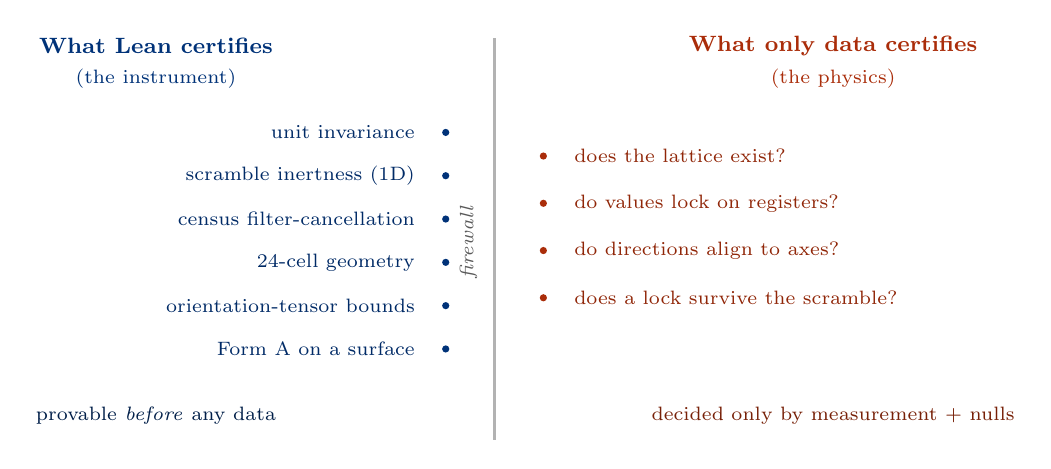
\begin{tikzpicture}[font=\footnotesize, >=Stealth,
   lbl/.style={align=center, inner sep=3pt}]
  % wall
  \draw[very thick, gray!60] (0,-2.5) -- (0,2.6);
  \node[gray!70!black, rotate=90] at (-0.33,0) {\scriptsize\itshape firewall};
  % LEFT: what Lean certifies
  \node[lbl, kishblue, font=\footnotesize\bfseries] at (-4.3,2.5) {What Lean certifies};
  \node[lbl, kishblue] at (-4.3,2.08) {\scriptsize(the instrument)};
  \foreach \y/\t in {1.4/unit invariance, 0.85/scramble inertness (1D),
                     0.3/census filter-cancellation, -0.25/24-cell geometry,
                     -0.8/orientation-tensor bounds, -1.35/Form A on a surface} {
    \node[lbl, left, kishblue!85!black] at (-0.9,\y) {\scriptsize \t};
    \fill[kishblue] (-0.62,\y) circle (1.3pt);
  }
  \node[lbl, kishblue!60!black] at (-4.3,-2.2) {\scriptsize provable \emph{before} any data};
  % RIGHT: what only data certifies
  \node[lbl, cruciblered, font=\footnotesize\bfseries] at (4.3,2.5) {What only data certifies};
  \node[lbl, cruciblered] at (4.3,2.08) {\scriptsize(the physics)};
  \foreach \y/\t in {1.1/does the lattice exist?, 0.5/do values lock on registers?,
                     -0.1/do directions align to axes?, -0.7/does a lock survive the scramble?} {
    \node[lbl, right, cruciblered!85!black] at (0.9,\y) {\scriptsize \t};
    \fill[cruciblered] (0.62,\y) circle (1.3pt);
  }
  \node[lbl, cruciblered!70!black] at (4.3,-2.2) {\scriptsize decided only by measurement + nulls};
\end{tikzpicture}
\caption{The firewall. Everything on the left is a mathematical property of the instrument and is
provable, in principle, with no data at all --- this is Lean's domain. Everything on the right is an
empirical property of the world and is decided only by data and the nulls. Lean can never cross the
wall, and the programme never lets ``verified'' pretend it has.}
\end{figure}

\section{How Lean Works, Briefly}

Lean is an open-source functional programming language and interactive theorem prover, built around a
deliberately \emph{tiny} trusted kernel: every proof, however it was produced, is ultimately reduced
to steps that small kernel checks. Its mathematical library, Mathlib, contains millions of lines of
formalized mathematics --- groups, root systems, quaternions, linear algebra, measure theory --- that
a new proof can build on. The same machinery underwrites automated-reasoning efforts at the major AI
labs, where machine-checkable proof is the scoring standard precisely because it cannot be faked.

\begin{figure}[H]
\centering
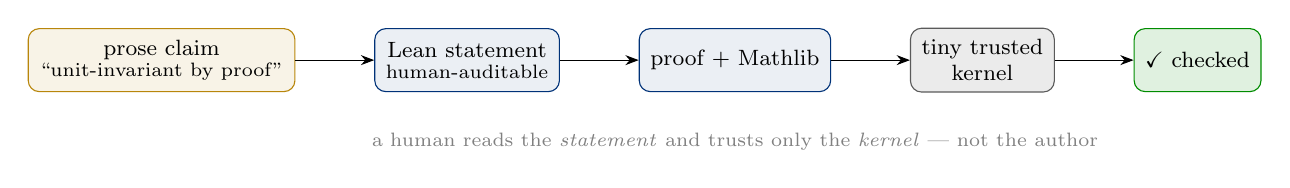
\begin{tikzpicture}[font=\footnotesize, >=Stealth, node distance=5mm,
  b/.style={draw, rounded corners, align=center, inner sep=4pt, minimum height=8mm}]
  \node[b, fill=goldseal!10, draw=goldseal] (claim) {prose claim\\[-2pt]\scriptsize ``unit-invariant by proof''};
  \node[b, fill=kishblue!8, draw=kishblue, right=10mm of claim] (stmt) {Lean statement\\[-2pt]\scriptsize human-auditable};
  \node[b, fill=kishblue!8, draw=kishblue, right=10mm of stmt] (mathlib) {proof + Mathlib};
  \node[b, fill=formgray!12, draw=formgray, right=10mm of mathlib] (kernel) {tiny trusted\\ kernel};
  \node[b, fill=signalgreen!12, draw=signalgreen, right=10mm of kernel] (qed) {$\checkmark$ checked};
  \draw[->] (claim) -- (stmt); \draw[->] (stmt) -- (mathlib);
  \draw[->] (mathlib) -- (kernel); \draw[->] (kernel) -- (qed);
  \node[align=center, gray, below=4mm of mathlib] {\scriptsize a human reads the \emph{statement} and trusts only the \emph{kernel} --- not the author};
\end{tikzpicture}
\caption{From claim to check. A prose claim becomes a precise Lean statement a human can read and
agree is the right thing to prove; the proof is then reduced, through Mathlib, to steps a tiny fixed
kernel verifies. If it compiles, the theorem holds. Reputation plays no part.}
\end{figure}

\begin{warningbox}
\textbf{A fitting coincidence.} Lean~4's build tool is named \textbf{Lake} (``Lean~Make''); its
projects are configured by a \texttt{lakefile}. We have built \emph{lakes} of data for fifteen
volumes; the proof layer, it turns out, builds with Lake too. The deeper fit is real, not just the
name: Lean's whole design is a \emph{tiny trusted core that checks everything else} --- the same
principle as our fingerprints, our strict input contract, and ``the engine decides the truth.''
\end{warningbox}

\section{The Pre-Registered Target Theorems}

Filed before a line of Lean is written. These are the obligations the proof module must discharge,
and any that resist --- most pointedly Form~A --- will be reported as open exactly as they stand.

\begin{predictionbox}
\textbf{Lean verification targets (VL-1 through VL-7), filed in Volume 14.}
\begin{enumerate}
    \item \textbf{Period-engine unit invariance.} For the period resultant $R$ and any scale $c>0$,
          \[ R(\{c\,x_j\}) = R(\{x_j\}), \]
          because $\ln(c x) = \ln c + \ln x$ adds a constant to every phase --- a global rotation
          the resultant magnitude cannot see.
    \item \textbf{Erratum 1 --- scramble inertness in 1D.} For any statistic $f$ that reads only the
          \emph{multiset} of scalars, and any permutation $\sigma$,
          \[ f\big(\sigma(x)\big) = f(x). \]
          The one-dimensional scramble is therefore inert by construction.
    \item \textbf{Census filter-cancellation.} For the census ratio
          $\rho = \max_{\mathcal{G}} P_{\mathrm{real}} / \max_{\mathcal{G}} P_{\mathrm{scr}}$, a
          filter applied identically to real and scramble that preserves the argmax leaves $\rho$
          unchanged (the result measured empirically in Appendix~A).
    \item \textbf{The 24-cell, as geometry.} The 24 vertices equal the $D_4$ root system and form the
          binary tetrahedral group of order $24$; the symmetry group $F_4$ has order $1152$; the
          projection to $S^2$ yields the $12$ cuboctahedral axes. (Mathlib carries quaternions, finite
          groups, and root systems; these are among the most tractable targets.)
    \item \textbf{Orientation-tensor bounds.} The tensor $\mathbf{T} = \tfrac1n\sum_j \uvec{v}_j
          \uvec{v}_j^{\!\top}$ is symmetric positive-semidefinite with $\operatorname{tr}\mathbf{T}=1$,
          eigenvalues $\tau_i \in [0,1]$, and isotropy $\Rightarrow \tau_1=\tau_2=\tau_3=\tfrac13$.
    \item \textbf{Alignment-score properties.} The lattice alignment $a_j = \max_k |\uvec{v}_j \cdot
          \mathbf{n}_k| \in [0,1]$ is rotation-equivariant: $a(\mathbf{Q}\uvec{v};\,\mathbf{Q}\mathbf{n})
          = a(\uvec{v};\,\mathbf{n})$ for any rotation $\mathbf{Q}$.
    \item \textbf{Form A on a surface (flagship, open).} State the one-dimensional transform-artifact
          theorem formally, then prove or refute its extension to a surface. A Lean proof would close
          the \texttt{FORM\_A\_UNCLEARED} gate with machine-checked certainty --- stronger than any
          prose or model-assisted derivation.
\end{enumerate}
\end{predictionbox}

\begin{warningbox}
\textbf{Order of attack.} VL-1 through VL-3 are the invariance quartet's core --- short proofs that
harden claims already in print, and the right first commits. VL-4 through VL-6 verify the vector
engine's foundations \emph{before} the engine is built, which is the pre-registration law applied to
the proof layer. VL-7, Form~A, is the prize, and it is allowed to stay open as long as it must.
\end{warningbox}

\section{The Shape of One Theorem}

To make the commitment concrete rather than a promise, here is Erratum~1 (VL-2) in Lean. The idea is
small and exact: a statistic that reads only the \emph{multiset} of scalars cannot see order, so a
permutation of the sample --- the scramble --- cannot move it.

\begin{lstlisting}[style=lean, caption={VL-2, the shape of it. Schematic Lean 4; Mathlib lemma names may need adjustment on first compile.}, captionpos=b]
-- Erratum 1: a lock statistic that reads only the MULTISET of scalars
-- is blind to order, so any scramble (a permutation of the sample)
-- leaves it unchanged -- the scramble is inert in one dimension.

structure LockStat where
  f : Multiset ℝ → ℝ            -- the statistic sees the multiset, not the order

theorem scramble_inert_1d
    (S : LockStat) (xs σ : List ℝ) (h : σ ~ xs) :   -- σ is a permutation of xs
    S.f ↑σ = S.f ↑xs :=
  congrArg S.f (Multiset.coe_eq_coe.mpr h)           -- equal multisets ⟩ equal value
\end{lstlisting}

\begin{derivbox}
What the proof says, in words: the hypothesis \texttt{h} states that $\sigma$ is a
permutation of the sample. Casting both lists to multisets (the $\uparrow$ coercion) erases order, so
the two multisets are \emph{equal}; applying the statistic to equal inputs gives equal outputs. Three
lines, and the kernel checks every one. The same discipline applied to VL-1 would leave a single open
goal marked \texttt{sorry} --- Lean's honest placeholder for ``not yet proved'' --- which is exactly
how a pre-registered-but-unproved obligation should appear on the record.
\end{derivbox}

\section{Scope and Honest Limits}

\begin{correctionbox}
\textbf{What Lean will and will not reach, stated in advance.}
\begin{itemize}
    \item \textbf{Strong where we start.} Mathlib's algebra and geometry are deep, so the invariance
          quartet (VL-1--3) and the 24-cell facts (VL-4) are genuinely tractable.
    \item \textbf{Thin where the distributions live.} The asymptotic distributions --- the Rayleigh
          $3nR^2 \sim \chi^2_3$, the Bingham and Watson laws --- are heavy to formalize and may not
          exist in Mathlib. We do not pretend those will be verified soon; we scope to the algebraic
          and geometric statements first and say so.
    \item \textbf{Verification, not discovery.} Lean certifies what we have reasoned; it will not find
          new physics, and it cannot rescue a null. The data still rules.
    \item \textbf{The firewall again.} Nothing Lean proves is evidence for the lattice. Every verified
          theorem is a statement about the instrument.
\end{itemize}
\end{correctionbox}

\section{What This Commits Us To}

\begin{predictionbox}
A Lean~4 proof module, built with Lake and depending on Mathlib, will live in the project repository
beside the Python engines, fingerprinted like everything else. It will discharge VL-1 through VL-6 as
they are proved, carry VL-7 (Form~A) openly until it is closed, and mark every unproved obligation
with \texttt{sorry} so the state of the proof is never misrepresented. The module certifies the
instrument; the lakes and the nulls, as always, are what speak to the physics.
\end{predictionbox}

\begin{center}
\vspace{0.5em}
\itshape
We built engines that measure, and nulls that can say no. Now we add a layer that lets anyone check
the mathematics of the measuring itself --- not by trusting us, but by trusting a kernel that trusts
no one. The ruler will be provably straight. Whether it finds the lattice is still, and always, for
the data to say.
\vspace{0.5em}
\end{center}

\section*{Sources for this Appendix}
\addcontentsline{toc}{section}{Sources for this Appendix}

\begin{itemize}
    \item de Moura, L., \& Ullrich, S. (2021). \textit{The Lean 4 Theorem Prover and Programming
          Language}. In \textit{Automated Deduction --- CADE 28}, LNCS 12699, 625--635. Springer.
    \item The mathlib Community (2020). \textit{The Lean Mathematical Library}. In \textit{Proceedings
          of CPP 2020}, 367--381. ACM. \url{https://leanprover-community.github.io/}
    \item Lean 4 and the Lake build system. \url{https://lean-lang.org/}
    \item Google DeepMind (2024). \textit{AlphaProof}: formal mathematical reasoning with Lean.
          \url{https://deepmind.google/} \; \textit{(Representative of machine-checked proof as the
          scoring standard in automated reasoning.)}
\end{itemize}


% Guitar graphic - series ender
\begin{figure}[H]
\centering
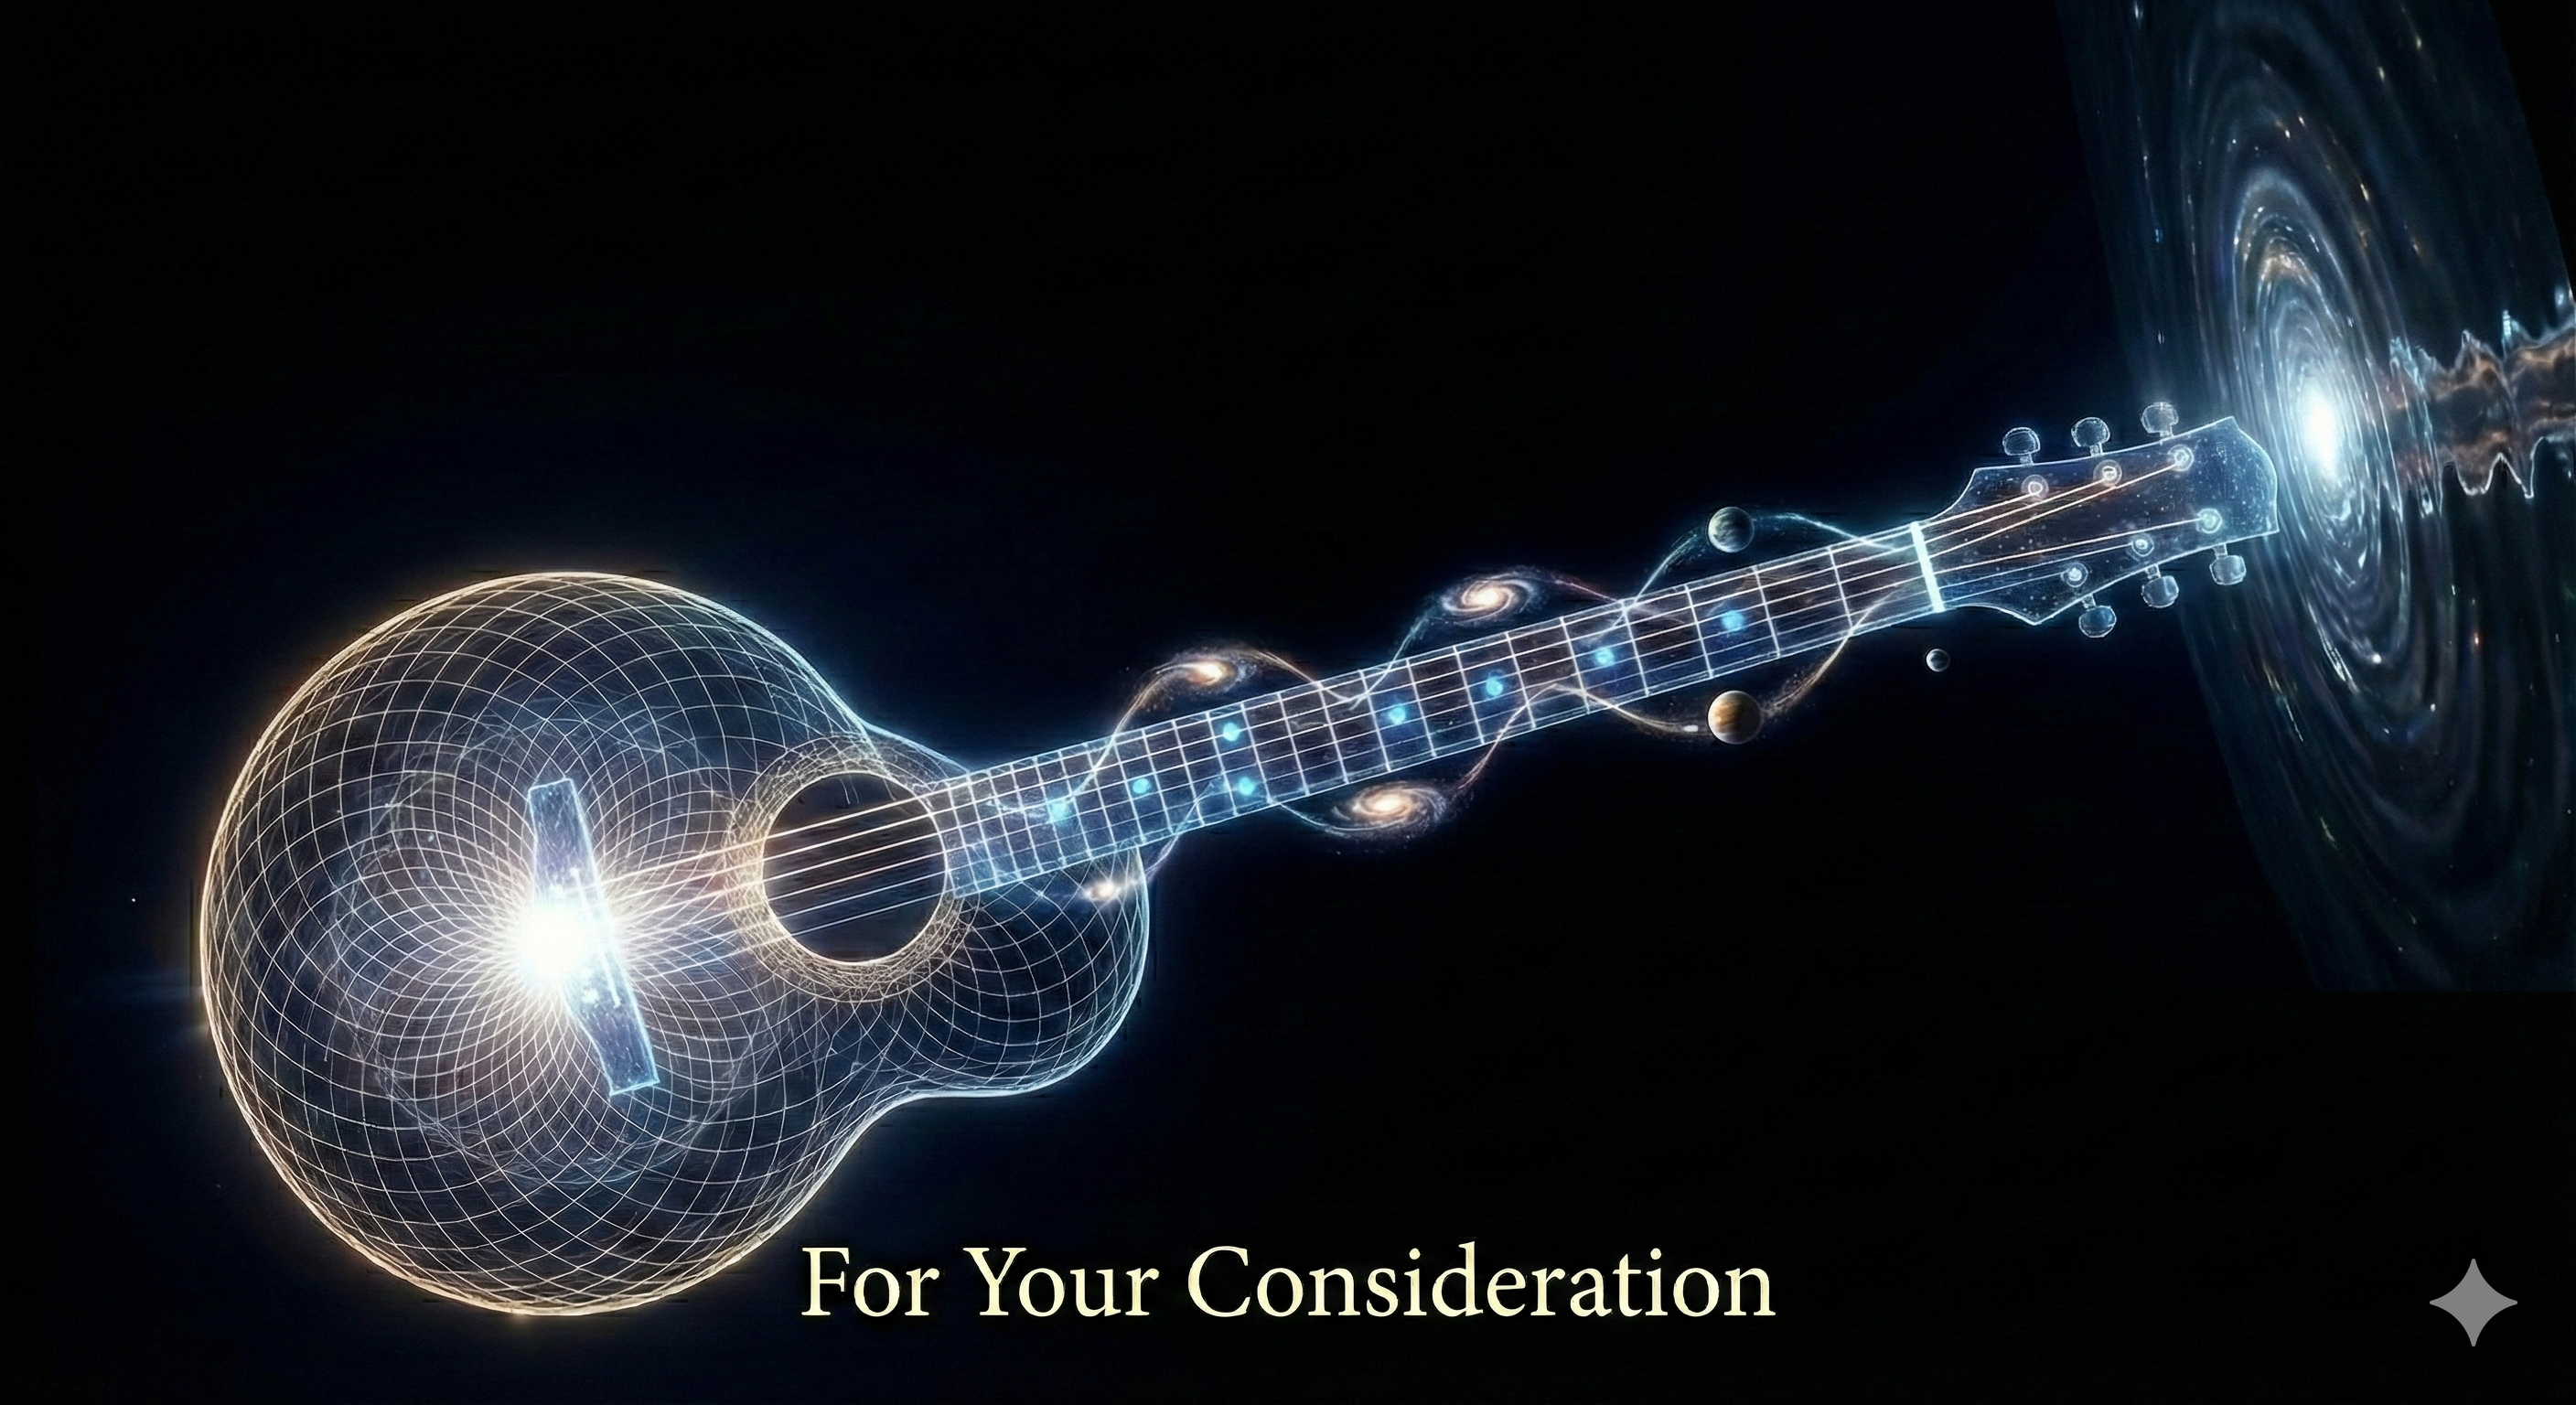
\includegraphics[width=0.85\textwidth]{Headers/ConclusionGuitar.png}
\end{figure}

\begin{center}
There is no Noise only Data. Remove the filters and see the Universe raw.
\end{center}

\end{document}